 % arara: clean: { files: [thesis.aux, thesis.bbl, thesis.blg, thesis.dvi, thesis.fdb_latexmk, thesis.fls, thesis.idx, thesis.ilg, thesis.ind, thesis.lof, thesis.log, thesis.lot, thesis.nlo, thesis.nls, thesis.out, thesis.pdf, thesis.ps, thesis.toc]}
% arara: latex:  { shell: yes }
% arara: bibtex
% arara: nomencl
% arara: latex
% arara: makeindex
% arara: latex:  { shell: yes }
% arara: dvips
% arara: ps2pdf

% ******************************* PhD Thesis Template **************************
% Please have a look at the README.md file for info on how to use the template

	
	
\documentclass[a4paper,12pt,times,numbered,index,print]{Classes/PhDThesisPSnPDF}
		
% ******************************************************************************
% ******************************* Class Options ********************************
% *********************** See README for more details **************************
% ******************************************************************************

% `a4paper'(The University of Cambridge PhD thesis guidelines recommends a page
% size a4 - default option) or `a5paper': A5 Paper size is also allowed as per
% the Cambridge University Engineering Deparment guidelines for PhD thesis
%
% `11pt' or `12pt'(default): Font Size 10pt is NOT recommended by the University
% guidelines
%
% `oneside' or `twoside'(default): Printing double side (twoside) or single
% side.
%
% `print': Use `print' for print version with appropriate margins and page
% layout. Leaving the options field blank will activate Online version.
%
% `index': For index at the end of the thesis
%
% `draft': For draft mode without loading any images (same as draft in book)
%
% `draftmode': Special draft mode with line numbers, images, and water mark with
% timestamp and custom text. Position of the text can also be modified.
%
% `abstract': To generate only the title page and abstract page with
% dissertation title and name, to submit to the Student Registry
%
% `chapter`: This option enables only the specified chapter and it's references
%  Useful for review and corrections.
%
% ************************* Custom Page Margins ********************************
%
% `custommargin`: Use `custommargin' in options to activate custom page margins,
% which can be defined in the preamble.tex. Custom margin will override
% print/online margin setup.
%
% *********************** Choosing the Fonts in Class Options ******************
%
% `times' : Times font with math support. (The Cambridge University guidelines
% recommend using times)
%
% `fourier': Utopia Font with Fourier Math font (Font has to be installed)
%            It's a free font.
%
% `customfont': Use `customfont' option in the document class and load the
% package in the preamble.tex
%
% default or leave empty: `Latin Modern' font will be loaded.
%
% ********************** Choosing the Bibliography style ***********************
%
% `authoryear': For author-year citation eg., Krishna (2013)
%
% `numbered': (Default Option) For numbered and sorted citation e.g., [1,5,2]
%
% `custombib': Define your own bibliography style in the `preamble.tex' file.
%              `\RequirePackage[square, sort, numbers, authoryear]{natbib}'.
%              This can be also used to load biblatex instead of natbib
%              (See Preamble)
%
% **************************** Choosing the Page Style *************************
%
% `default (leave empty)': For Page Numbers in Header (Left Even, Right Odd) and
% Chapter Name in Header (Right Even) and Section Name (Left Odd). Blank Footer.
%
% `PageStyleI': Chapter Name next & Page Number on Even Side (Left Even).
% Section Name & Page Number in Header on Odd Side (Right Odd). Footer is empty.
%
% `PageStyleII': Chapter Name on Even Side (Left Even) in Header. Section Number
% and Section Name in Header on Odd Side (Right Odd). Page numbering in footer


% ********************************** Preamble **********************************
% Preamble: Contains packages and user-defined commands and settings
% ******************************************************************************
% ****************************** Custom Margin *********************************

% Add `custommargin' in the document class options to use this section
% Set {innerside margin / outerside margin / topmargin / bottom margin}  and
% other page dimensions
\ifsetCustomMargin
  \RequirePackage[left=37mm,right=30mm,top=35mm,bottom=30mm]{geometry}
  \setFancyHdr % To apply fancy header after geometry package is loaded
\fi

% *****************************************************************************
% ******************* Fonts (like different typewriter fonts etc.)*************

% Add `customfont' in the document class option to use this section

\ifsetCustomFont
  % Set your custom font here and use `customfont' in options. Leave empty to
  % load computer modern font (default LaTeX font).
  \RequirePackage{helvet}
\fi

% *****************************************************************************
% **************************** Custom Packages ********************************

% ************************* Algorithms and Pseudocode **************************

%\usepackage{algpseudocode}


% ********************Captions and Hyperreferencing / URL **********************

% Captions: This makes captions of figures use a boldfaced small font.
%\RequirePackage[small,bf]{caption}

\RequirePackage[labelsep=space,tableposition=top]{caption}
\renewcommand{\figurename}{Fig.} %to support older versions of captions.sty


% *************************** Graphics and figures *****************************

%\usepackage{rotating}
%\usepackage{wrapfig}

% Uncomment the following two lines to force Latex to place the figure.
% Use [H] when including graphics. Note 'H' instead of 'h'
%\usepackage{float}
%\restylefloat{figure}

% Subcaption package is also available in the sty folder you can use that by
% uncommenting the following line
% This is for people stuck with older versions of texlive
%\usepackage{sty/caption/subcaption}
\usepackage{subcaption}

% ********************************** Tables ************************************
\usepackage{booktabs} % For professional looking tables
\usepackage{multirow}

%\usepackage{multicol}
%\usepackage{longtable}
%\usepackage{tabularx}


% ***************************** Math and SI Units ******************************

\usepackage{amsfonts}
\usepackage{amsmath}
\usepackage{amssymb}
\usepackage{siunitx} % use this package module for SI units


% ******************************* Line Spacing *********************************

% Choose linespacing as appropriate. Default is one-half line spacing as per the
% University guidelines

% \doublespacing
% \onehalfspacing
% \singlespacing


% ************************ Formatting / Footnote *******************************

% Don't break enumeration (etc.) across pages in an ugly manner (default 10000)
%\clubpenalty=500
%\widowpenalty=500

%\usepackage[perpage]{footmisc} %Range of footnote options


% *****************************************************************************
% *************************** Bibliography  and References ********************

%\usepackage{cleveref} %Referencing without need to explicitly state fig /table

%\usepackage[style=numeric-comp,maxnames=7,natbib=true,backend=bibtex,bibstyle=numeric]{biblatex}
%\addbibresource{sangphan.bib}


% Add `custombib' in the document class option to use this section
\ifuseCustomBib
   \RequirePackage[square, sort, numbers, authoryear]{natbib} % CustomBib

% If you would like to use biblatex for your reference management, as opposed to the default `natbibpackage` pass the option `custombib` in the document class. Comment out the previous line to make sure you don't load the natbib package. Uncomment the following lines and specify the location of references.bib file


%\RequirePackage[backend=bibtex, style=numeric-comp, citestyle=numeric, sorting=nty, natbib=true]{biblatex}
%\bibliography{References/references} %Location of references.bib only for biblatex


\fi

% changes the default name `Bibliography` -> `References'
\renewcommand{\bibname}{References}


% *****************************************************************************
% *************** Changing the Visual Style of Chapter Headings ***************
% This section on visual style is from https://github.com/cambridge/thesis

% Uncomment the section below. Requires titlesec package.

%\RequirePackage{titlesec}
%\newcommand{\PreContentTitleFormat}{\titleformat{\chapter}[display]{\scshape\Large}
%{\Large\filleft{\chaptertitlename} \Huge\thechapter}
%{1ex}{}
%[\vspace{1ex}\titlerule]}
%\newcommand{\ContentTitleFormat}{\titleformat{\chapter}[display]{\scshape\huge}
%{\Large\filleft{\chaptertitlename} \Huge\thechapter}{1ex}
%{\titlerule\vspace{1ex}\filright}
%[\vspace{1ex}\titlerule]}
%\newcommand{\PostContentTitleFormat}{\PreContentTitleFormat}
%\PreContentTitleFormat


% ******************************************************************************
% ************************* User Defined Commands ******************************
% ******************************************************************************

% *********** To change the name of Table of Contents / LOF and LOT ************

%\renewcommand{\contentsname}{My Table of Contents}
%\renewcommand{\listfigurename}{My List of Figures}
%\renewcommand{\listtablename}{My List of Tables}


% ********************** TOC depth and numbering depth *************************

\setcounter{secnumdepth}{2}
\setcounter{tocdepth}{2}


% ******************************* Nomenclature *********************************

% To change the name of the Nomenclature section, uncomment the following line

%\renewcommand{\nomname}{Symbols}


% ********************************* Appendix ***********************************

% The default value of both \appendixtocname and \appendixpagename is `Appendices'. These names can all be changed via:

%\renewcommand{\appendixtocname}{List of appendices}
%\renewcommand{\appendixname}{Appndx}

% ******************************** Draft Mode **********************************

% Uncomment to disable figures in `draftmode'
%\setkeys{Gin}{draft=true}  % set draft to false to enable figures in `draft'

% These options are active only during the draft mode
% Default text is "Draft"
%\SetDraftText{DRAFT}

% Default Watermark location is top. Location (top/bottom)
%\SetDraftWMPosition{bottom}

% Draft Version - default is v1.0
%\SetDraftVersion{v1.1}

% Draft Text grayscale value (should be between 0-black and 1-white)
% Default value is 0.75
%\SetDraftGrayScale{0.8}


%% Todo notes functionality
%% Uncomment the following lines to have todonotes.

%\ifsetDraft
%	\usepackage[colorinlistoftodos]{todonotes}
%	\newcommand{\mynote}[1]{\todo[author=kks32,size=\small,inline,color=green!40]{#1}}
%\else
%	\newcommand{\mynote}[1]{}
%	\newcommand{\listoftodos}{}
%\fi

% Example todo: \mynote{Hey! I have a note}

\usepackage{epigraph}

% ************************ Thesis Information & Meta-data **********************
% Thesis title and author information, refernce file for biblatex
% ************************ Thesis Information & Meta-data **********************
%% The title of the thesis
\title{Multimedia Event Detection Using Segment-based Approach}
%\texorpdfstring is used for PDF metadata. Usage:
%\texorpdfstring{LaTeX_Version}{PDF Version (non-latex)} eg.,
%\texorpdfstring{$sigma$}{sigma}

%% Subtitle (Optional)
%\subtitle{Using the CUED template}

%% The full name of the author
\author{PHAN LE SANG}

%% Department (eg. Department of Engineering, Maths, Physics)
\dept{Department of Informatics}

\school{School of Multidisciplinary Sciences}

%% University and Crest
\university{The Graduate University for Advanced Studies (SOKENDAI)}
\crest{
\includegraphics[width=0.25\textwidth]{Sokendai}}

%% You can redefine the submission text:
% Default as per the University guidelines:
% ``This dissertation is submitted for the degree of''
%\renewcommand{\submissiontext}{change the default text here if needed}

%% Full title of the Degree
\degreetitle{Doctor of Philosophy}

%% College affiliation (optional)
%\college{King's College}

%% Submission date
% Default is set as {\monthname[\the\month]\space\the\year}
%\degreedate{September 2014} 

%% Meta information
\subject{LaTeX} \keywords{{LaTeX} {PhD Thesis} {Informatics} {The Graduate University for Advanced Studies (SOKENDAI)}}


% ***************************** Abstract Separate ******************************
% To printout only the titlepage and the abstract with the PhD title and the
% author name for submission to the Student Registry, use the `abstract' option in
% the document class.

\ifdefineAbstract
 \pagestyle{empty}
 \includeonly{Declaration/declaration, Abstract/abstract}
\fi

% ***************************** Chapter Mode ***********************************
% The chapter mode allows user to only print particular chapters with references
% Title, Contents, Frontmatter are disabled by default
% Useful option to review a particular chapter or to send it to supervisior.
% To use choose `chapter' option in the document class

\ifdefineChapter
 \includeonly{Chapter3/chapter3}
\fi

% ******************************** Front Matter ********************************
\begin{document}
	

\frontmatter

\begin{titlepage}
  \maketitle
\end{titlepage}

\begin{spacing}{1.5}

%\renewcommand{\cleardoublepage}{}
	
% ******************************* Thesis Dedidcation ********************************

\begin{dedication} 

for my loving parents \dots

\end{dedication}


%\include{Declaration/declaration}
% ************************** Thesis Acknowledgements **************************

\begin{acknowledgements}      


This dissertation would have not finished without the support of many people.

I have been very fortunate to be supervised by Prof. Shin'ichi Satoh, who has a profound knowledge in my research area, who is always nice and provides whatever support for his students.

I am grateful to be co-supervised by Prof. Duy-Dinh Le, who always takes care of my research progress as well as other members in our group. I have been extremely lucky to be your student.     

I also want to send my sincere gratitude to other professors in my Ph.D committee including Prof. Akihiro Sugimoto, Prof. Imari Sato and Prof. Gene Cheung. Without your valuable comments, my PhD would have taken longer to complete. 

I would like to thank all of my friends who are always encouraging me to keep studying. Especially, I must thank my friends at National Institute of Informatics, Japan who have been my companies and/or my collaborators on the way pursuing my Ph.D.  

Finally, I want to thank my parents and my love for your enduring support and love. 

\end{acknowledgements}

% ************************** Thesis Abstract *****************************
% Use `abstract' as an option in the document class to print only the titlepage and the abstract.
\begin{abstract}


Recognizing event in unconstrained videos is one of the most important tasks in multimedia retrieval. It has many potential applications such as video indexing, searching, and event recounting. However, this is a challenging task due to the large content variation and uncontrolled capturing condition. This leads to the fact that these videos often contain irrelevant information to the event of interest. The straightforward way to solve this problem is to decompose the original video into smaller segments and build the event detectors from these segment representations. This dissertation follows the aforementioned direction to study event detection methods in real videos. Essentially, we study three complementary approaches including \textit{feature representation}, \textit{feature aggregation} and \textit{feature learning}. 

In the first approach, we propose to use the segment-based (\textbf{SB}) \textit{feature representation} to overcome the limitation of the traditional video-based approach. In the video-based approach, local features are extracted from the entire video and then aggregated to form the final video representation. However, this video-based representation is ineffective when used for realistic videos because the video length can be very different and the clues to determine an event may happen in only a small segment of the entire video. To handle this problem, our segment-based divides the original videos into segments for feature extraction and classification, while still keeping the evaluation at the video level. We investigate several strategies to divide a video into segments including non-overlapping uniform segment sampling, overlapping uniform segment sampling, and segments that based on the shot boundary detection. We also study the optimal segment length for event detection, which is close to the mean average length of the training videos.

The second approach handles the aforementioned problem by proposing a new video pooling strategy for \textit{feature aggregation}. We consider a video as a layered structure where the lowest layer are frames, the top layer is the entire video, and the middle layers are the sequences of consecutive frames or the concatenation of lower layers. While it is easy to find local discriminative features in video from lower layers, it is non-trivial to aggregate these features into a discriminative video representation. In literature, people often use sum pooling to obtain reasonable recognition performance on artificial videos. However, the sum pooling technique does not work well on complex videos because the region of interests may reside within some middle layers. In this approach, we leverage the layered structure of video to propose a new video pooling method, named sum-max video pooling (\textbf{SM}), to handle this problem. Basically, we apply sum pooling at the low layer representation while using max pooling at the high layer representation. Sum pooling is used to keep sufficient relevant features at the low layer, while max pooling is used to retrieve the most relevant features at the high layer, therefore it can discard irrelevant features in the final video representation. 
	
In the third approach, we focus on \textit{feature learning} method to learn the key segments for video representation. In fact, a complex event can be recognized by observing necessary evidences. It is not easy to locate supportive evidences because they can happen anywhere in a video. A straightforward solution is to decompose the video into several segments and search for the evidences in each segment. This approach is based on the assumption that segment annotation can be assigned from its video label. However, this is a weak assumption because the importance of each segment is not considered. On the other hand, the importance of a segment to an event can be obtained by matching its detected concepts against the evidential description of that event. Leveraging this prior knowledge, we propose a new method, Event-driven Multiple Instance Learning (\textbf{EDMIL}), to learn the key evidences for event detection. We treat each segment as an instance and quantize the instance-event similarity into different levels of relatedness. Then the instance labels are learned by jointly optimizing the instance classifier and its related level. Finally the optimal instance classifiers are used to detect event.

We verify the effectiveness of our approaches on the large scale TRECVID Multimedia Event Detection 2010, 2011 and 2012 datasets. Our approaches can not only detect event, but also provide evidences for event detection. Compared to other segment-based approaches, our solutions achieve significant improvements. For example, when comparing in the MED 2011 dataset with a same setting, the baseline method (traditional video-based approach) has the average precision of 6.74\%, while our methods (SB, SM and EDMIL) have the performance of 8.26\%, 6.92\% and 9.68\% respectively.

\end{abstract}


% *********************** Adding TOC and List of Figures ***********************

\tableofcontents
\listoffigures
\listoftables

%\clearpage

% \printnomencl[space] space can be set as 2em between symbol and description
%\renewcommand\nomname{Abbreviations} 
% {\clearpage\pagenumbering{roman}\pagestyle{plain}}
% {\clearpage\pagenumbering{arabic}}
%\printnomencl[3em]

\renewcommand{\thepage}{\roman{page}}
\renewcommand\nomname{Abbreviations}
\printnomenclature


%\printnomencl

% ******************************** Main Matter *********************************
\mainmatter

\chapter{Introduction}
\label{chapter1}

%\setlength{\epigraphrule}{0pt}
\epigraph{\textit{The moment you doubt whether you can fly, you cease for ever to be able to do it.}}{ -- J.M. Barrie, \textit{Peter Pan}}


% **************************** Define Graphics Path **************************
\ifpdf
    \graphicspath{{Chapter1/Figs/Raster/}{Chapter1/Figs/PDF/}{Chapter1/Figs/}}
\else
    \graphicspath{{Chapter1/Figs/Vector/}{Chapter1/Figs/}}
\fi

\section{Motivations}
The evolution of internet has been changing our daily life. According to a report by the Internet World Stats \cite{Internet1}, there is now more than 3 billions internet users, accounting for 40\% of the world's population. The number of internet users are increasing rapidly and also keep producing a huge amount of internet data. It is important to analyze these data because it can provide valuable information about our daily activities. Among many interesting problems that need to be investigated, recognizing event in internet videos has been drawing a lot of attention in recent years \cite{natarajan2012multimodal,sun2013large,habibian2013recommendations,myers2014evaluating}. 

Recognizing event refers to the process of automatically identifying video clips that contain a particular event of interest. This is a challenging problem because we need to build computer system to recognize event not only from video metadata but also from its content. The detail definition of this task and its challenges will be described in Section \ref{c1_problemdefinition} and Section \ref{c1_challenges} respectively. 

Event recognition technologies are mainly employed in \index{video retrieval} video retrieval systems to facilitate the retrieving progress. A video retrieval system that equipped such technologies can have numerous applications such as video search, video recommendation and video filtering. For example, below are some application scenarios:

\begin{itemize}
	\item \textbf{Video search.}\index{video search} This is an important function in most of video sharing websites. Most of the time, these websites only provide a search interface that supports text queries. However, in order to do that, videos must have already been indexed based on its content and other metadata \cite{zhang1997integrated}. Using the provided interface, user can search for a specific tutorial such as ``how to make a cake'',  ``how to repair an appliance''; or some specific entertainment videos such as ``a dog show'' and ``doing a magic trick''.
	\item \textbf{Video recommendation.}\index{video recommendation} It is also very important for video sharing websites to recommend videos that may appeal to the user. The longer the user stay on their websites, the higher the benefit. The recommendation is often based on the user's favorite videos or recently watched videos \cite{davidson2010youtube,mei2007automatic}. From these input videos, the system will search for similar videos through their database within a short time. For example, when the user watch a video of ``how to drive a car'', they may also expected to watch similar events such as ``how to park a car'' and ``common driving mistakes''.
	\item \textbf{Video filtering.} In contrast to video recommendation, video filtering is also an important application of event detection technologies. There are certain event that the managers do not want them to be public, especially when a government want to establish a video censorship. For example, videos that teach ``how to make a bomb'' or ``how to commit a suicide'' should be removed from the retrieval results. 

	Zillmann and Weaver \cite{JASP:JASP145} show that human tend to have violent responses when watching violent movies. In this case, event detection technology can be applied to filter out violent scenes \index{violent scene detection} in a movies. This technology has been employed in Facebook platform \cite{Internet3} to prevent the spread of a particular video over the internet, or to restrict the video from a particular type of audiences such as children, as shown in Fig. \ref{c1_facebook}. 
	
	\begin{figure}
		\centering
		
\includegraphics[width=1\textwidth]{facebook.png}
		\caption{Facebook has been placing warnings over violent videos posted to its site.}
		\label{c1_facebook}
	\end{figure}
	
\end{itemize}

Motivated by these interesting applications, this dissertation aims to develop technologies for building an automatic event detection system. We will describe more about our research scope in the next section.

\section{Problem Statement}
\label{c1_problemdefinition}
This dissertation addresses the problem of recognizing complex event in videos. Basically, it is the process of automatically identifying video clips that contain a particular event of interest. There are two important characteristics of our target problem. 

\begin{figure}
	\centering
	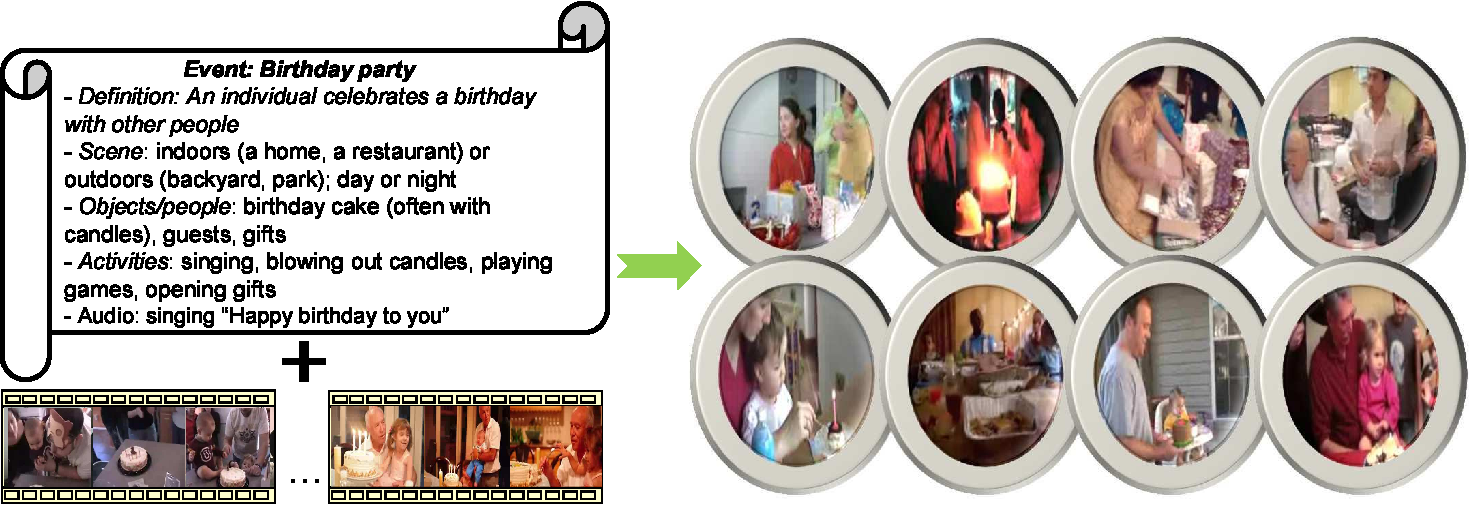
\includegraphics[width=1\textwidth]{eventdetection.pdf}
	\caption{Overview of an event detection from video system.}
	\label{c1_eventdetection}
\end{figure}

First, we are dealing with \textbf{complex event}. A complex event consists of various human activities and occurs in some particular settings. For example, ``changing a vehicle tire'' is an complex event that often happens at a garage or on street. This event contains several activities such as removing hubcap, turning lugwrench, unscrewing bolts and pulling rim out of tire. Complex event recognition differs from the traditional action recognition \index{action recognition} task in that it is the combination of multiple human actions or activities. It often contains various interactions between human and objects in different scenes. Therefore, a complex event video is often longer than a single action video. Moreover, action videos are often captured in controlled environment, while complex event videos are often recorded by internet users, which is uncontrolled or arbitrary environment. Figure \ref{c1_comparision} shows the difference of complex event and single action detection. The top images are sequence of actions that happens in a shoplifting event, while the bottom images are examples of single action in the classic KTH dataset. Note that for the shoplifting event, the sequence of actions needed to be recorded in exactly the order from left to right. That means we not only deal with multiple actions, but also need to take into account the order that these actions happen.

\begin{figure}
	\centering
	\begin{minipage}{.3\textwidth}
		\centering
		
\includegraphics[width=1\linewidth]{shoplifting1.jpg}
		\\
	Pick up an item
	\end{minipage}%
	\begin{minipage}{.3\textwidth}
		\centering
		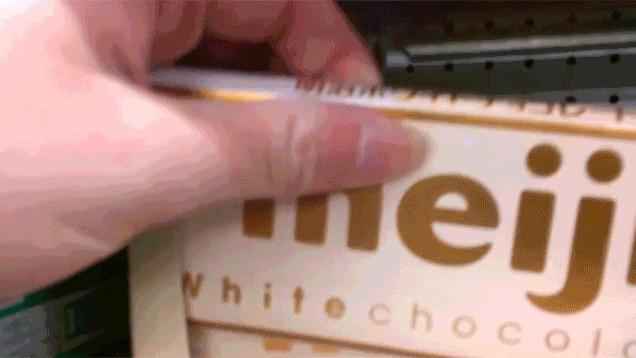
\includegraphics[width=1\linewidth]{shoplifting2.jpg}
		\\
	Keep it in a hidden place
		\end{minipage}
	\begin{minipage}{.3\textwidth}
		\centering
		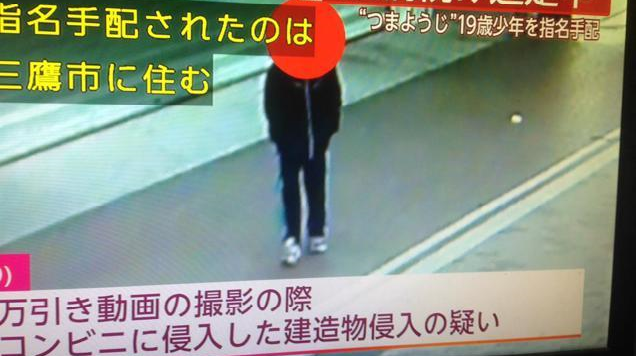
\includegraphics[width=1\linewidth]{shoplifting3.jpg}
		\\
		Get out successfully
	\end{minipage}
		
	\centering
	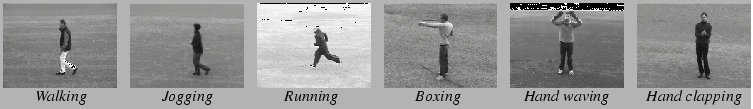
\includegraphics[width=1\textwidth]{kth.png}
	\caption{Top: sequence of actions in the shoplifting event. Bottom: Examples of single action detection in KTH dataset.}
	\label{c1_comparision}
\end{figure}

% % mentioned about CBVR 
Second, we are dealing with \textbf{multimedia data}. Internet videos can contain information from various mediums such as audio, visual and textual. Beside information from its content, internet videos often come with user-provided metadata description such as titles, tags and descriptions. Traditionally, videos are indexed and retrieved based on this metadata information. However, text-based video retrieval systems face an intrinsic limitation that is the semantic gap \index{semantic gap} between the content of the video and the information provided by the users. Moreover, this information is tend to be noisy and not always reliable. Therefore, we focus on utilizing multimedia data to build an effective event recognition system.

Due to the uncontrolled capturing condition of the complex videos, it is also interesting to know which parts of the video are important for recognizing event? How can we detect these parts? And suppose these parts do exist, how can we utilize them for complex event recognition? These challenging questions are also addressed in our dissertation.  

\section{Challenges}
\label{c1_challenges}
\begin{itemize}
	\item{\textbf{Large content variation.}} The large content variation refers to the diversity of a complex event. Even though an event only involve with some specific objects, activities and scenes, the variety among within these classes is also very high. For example, ``birthday party'' is a complex event. This event can be happen during day or night and set in indoor (a home, a restaurant) or outdoor (a backyard, a park) environment. Typically, in a birthday party, the presence of a birthday cake is of the utmost importance. However, in the real world setting, even the birthday cake can be very different from video to video. Figure \ref{c1_largecontent} shows some examples of birthday cake appear in internet videos. 
	\begin{figure}
		\centering
		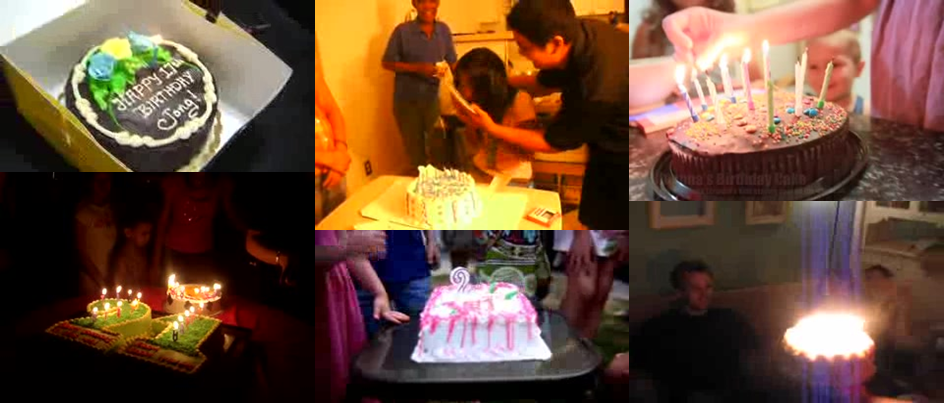
\includegraphics[width=1\textwidth]{largecontent.png}
		\caption{The large variation of birthday cake in the birthday party event.}
		\label{c1_largecontent}
	\end{figure}
	
	In terms of content variation, recognizing complex event is more challenging than other tasks such as instance search \index{instance search} or copy detection \index{copy detection}. The instance search task aims to search for a certain specific person, object or location. These instances can have different views but it must belong to the same target of interest in the real world. The target of copy detection task is a little bit more flexible. It aims to detect a video segment that is derived from another video. The copy video can be derived from the original video by means of transformations such as addition, deletion and modification. To this end, the complex event detection task has the utmost content variation.
	 
	\item{\textbf{Uncontrolled capturing condition.}} The uncontrolled capturing condition distinguish the complex event recognition task and the traditional action recognition task, which is often recorded in studio settings. As a result, techniques that work well for action recognition might no longer be effective for detecting complex event. For example, camera motion is one of the most frequent prominence in internet videos. Although popular motion features \index{motion feature} such as \nomenclature[-esurf]{ESURF}{Extended Speeded Up Robust Features} ESURF \cite{willems2008efficient}, \nomenclature[-stip]{STIP}{Spatial-temporal Interest Points} STIP \cite{Laptev03space-timeinterest} and \nomenclature[-hog3d]{HOG3G}{Histogram of 3D Gradients} HOG3D \cite{Klaser08BMVC} can effectively recognize action in studio videos, it shows limited performance in internet videos because it is not designed to handle camera motion. On the other hand, the Dense Trajectories feature proposed by Wang \cite{wang2013action} takes into account the camera motion and demonstrates superior performance.
	 
	One of the direct consequence of uncontrolled capturing condition is that user-generated videos often contain irrelevant information to the event of interest. In other words, different parts of the video have different levels of relatedness to a particular event. This leads to a challenging problem which is how to discard irrelevant information from the video representation. It is especially difficult when the annotation of each part of the video is almost not available. Figure \ref{c1_uncontrolled} shows some examples of noisy information in internet videos.
	
	\begin{figure}
		\centering
		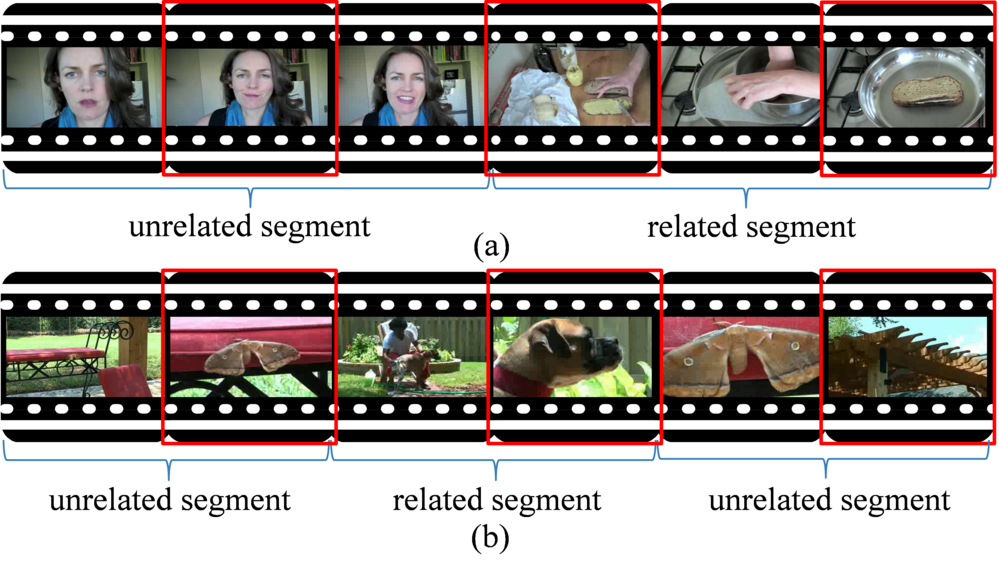
\includegraphics[width=1\textwidth]{teaser_image.png}
		\caption{(a) Example video for ``making a sandwich'' event: the related segment appears after a self-cam segment (unrelated); (b) example video for ``grooming an animal'' event: related segment is sandwiched between two unrelated segments. This kind of video is popular in realistic video datasets like MED. The frames with a red outlined box are examples of the extracted keyframes when using a keyframe-based approach, which suffers from both noise and missed extraction.}
		\label{c1_uncontrolled}
	\end{figure}
	 
	\item{\textbf{Near-miss videos.}} Near-miss video refers to a kind of video that is closely related to a particular event, however, it is not a positive instance of that event. Because a complex video is often composed by several objects or activities in some particular order, it might not be considered an event video if there is a lack of certain evidences. So a near-miss video can contain several evidences but not enough to define an event. This property of near-miss video often harm the performance of an event detection system. In fact, this kind of video is also prevalent in the setting of complex event recognition task. For example, ``Changing a vehicle tire'' is a complex event that involve one or more people to replace a tire on a vehicle. An event is not defined if the tire of the vehicle is not replaced. Examples of near-miss videos can be seen in Fig. \ref{c1_nearmiss}.
	
	\begin{figure}
		\centering
		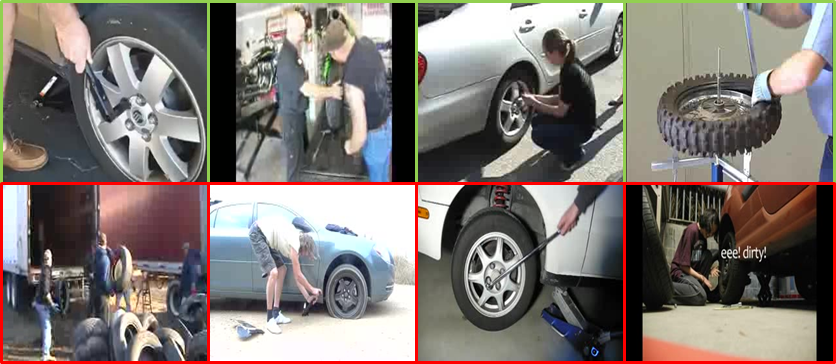
\includegraphics[width=1\textwidth]{near_miss.png}
		\caption{Example of near-miss video for ``Changing a vehicle tire'' event. The first row shows some positive videos. The second row shows near-miss videos, which is very easy to be confused with positive ones, even for human.}
		\label{c1_nearmiss}
	\end{figure}
		
	\item{\textbf{Large scale video database.}} Last but not least, we have to deal with big data as well. We have to accurately search for a particular event through a large video archive in a reasonable amount of time. In some complex event detection task such as \nomenclature[-trecvid]{TRECVID}{TREC Video Retrieval Evaluation} TRECVID Multimedia Event Detection (MED) \nomenclature[-med]{MED}{Multimedia Event Detection}\cite{over2014trecvid}, the evaluation time is also limited, which forces the participants to care about the efficiency of their systems. In this contest, the participants need to prepare their system that is able to search for event on large collection of around 200,000 Internet videos, or 8,000 hours of videos \cite{over2014trecvid}.
	
\end{itemize}

\section{Contributions}

The main challenge that is addressed in this dissertation is "uncontrolled capturing condition". This challenge differentiates complex videos from artificial or studio setting videos. The straightforward approach to handle this challenge is to decompose the original video into small video segments and search for event evidences in these small segments. By following this research direction, we made three main contributions in our dissertation:

\begin{itemize}
\item We propose a new \textit{feature representation} method, named segment-based representation (\textbf{SB}), to overcome the limitations of the traditional video-based approaches. The basic idea is to examine shorter segments instead of using the representative frames or entire video. We carry thorough experiments to verify our proposed method by investigating different strategies to decompose a video into segments. These strategies include uniform segment sampling and segments based on shot boundary detection.

\item We propose a new \textit{feature aggregation} method, called sum-max video pooling (\textbf{SM}), to deal with noisy information in complex videos. This pooling technique is based on the layer structure of video. Basically, we apply sum pooling at the low layer representation while using max pooling at the high layer representation. Sum pooling is used to keep sufficient relevant features at the low layer, while max pooling is used to retrieve the most relevant features at the high layer, therefore it can discard irrelevant features in the final video representation. 
	
\item We propose a new \textit{feature learning} method, named Event-driven Multiple Instance Learning (\textbf{EDMIL}), to learn key evidences for complex event detection. We treat each segment as an instance and model it in a multiple instance learning framework \cite{andrews2002support}, where each video is a ``bag''. The instance-event similarity is quantized into different levels of relatedness. Intuitively, the most (ir)relevant instances should have higher (dis)similarities. Therefore, we propose to learn the instance labels by jointly optimizing the instance classifier and its related level.
	
\end{itemize}

\section{Thesis Overview}

%\nomenclature[g-pi]{$\pi$}{ $\simeq 3.14\ldots$} to be listed after $\alpha$\nomenclature{$\alpha$}{The first letter of the greek alphabet} \index{MED}

The remaining of this dissertation is organized as follows:

\textit{Chapter \ref{chapter2}} introduces some background that is related to our research. This background encompasses an introduction to TRECVID MED task and dataset. It also provide basic knowledge about some low level features and feature encoding methods, which is necessary to re-implement our system. 

\textit{Chapter \ref{chapter3}} presents our segment-based approach for complex event detection. At first we introduce the video-based approach and some of its limitation. After that we present the segment-based approach with several strategies to decompose a video into segments.

\textit{Chapter \ref{chapter4}} presents our sum-max video pooling for complex event recognition. At first we introduce the layer structure of a video. Based on this layer structure, we propose a new video pooling technique which is a combination of sum pooling and max pooling.

\textit{Chapter \ref{chapter5}} presents our method to detect event using the evidential description of an event. We also present a method to calculate the similarity between a video segment and an event based on textual description. This method can also provide evidences for event detection.

\textit{Chapter \ref{chapter6}} concludes this dissertation by summarizing our contributions and discussing about the future work.

	\begin{figure}
		\centering
		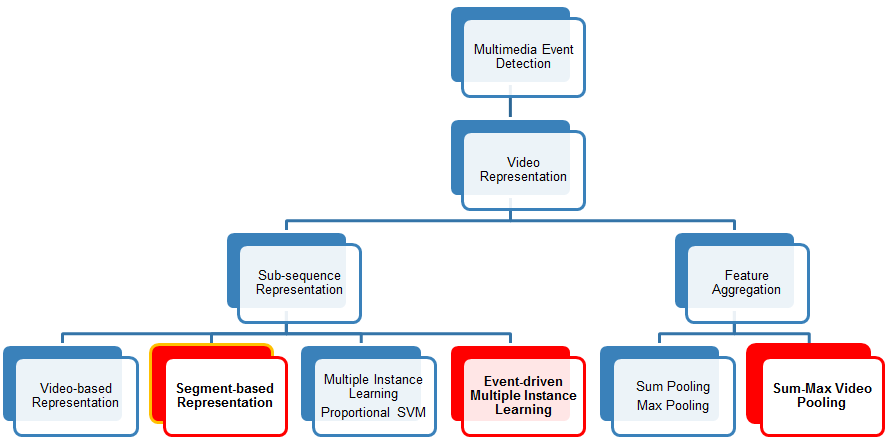
\includegraphics[width=1\textwidth]{outline.png}
		\caption{Outline of our thesis. Our contributions are highlighted in the red boxes.}
		\label{c1_outline}
	\end{figure}
	
\nomenclature[-sb]{SB}{Segment-based}
\nomenclature[-sm]{SM}{Sum-Max Video Pooling}
\nomenclature[-map]{MAP}{Mean Average Precision}
\nomenclature[-map]{SBD}{Shot Boundary Detection}


\chapter{Background}
\label{chapter2}
%\setlength{\epigraphrule}{0pt}
\epigraph{\textit{We can draw lessons from the past, but we cannot live in it.}}{ -- Lyndon B. Johnson}

% **************************** Define Graphics Path **************************
\ifpdf
    \graphicspath{{Chapter2/Figs/Raster/}{Chapter2/Figs/PDF/}{Chapter2/Figs/}}
\else
    \graphicspath{{Chapter2/Figs/Vector/}{Chapter2/Figs/}}
\fi


\section{TRECVID Multimedia Event Detection}

As introduced in Chapter \ref{chapter1}, complex event recognition is an important computer vision research with many potential applications. In 2010 TRECVID community has proposed a new task, named ``Multimedia Event Detection'' to advance the research and development in this area. The ultimate purpose of this task is to collect technologies for building a computer system that can quickly search for a particular event over a large video collection.
 
The task is defined as follows: ``Given an event kit, find all clips that contain the event in a video collection'' \cite{over2011trecvid}. The event kit provides the event definitions along with some example videos of each event. At first, MED task defines an event:\textit{ is a complex activity occurring at a specific place and time; involves people interacting with other people and/or objects; consists of a number of human actions, processes, and activities that are loosely or tightly organized and that have significant temporal and semantic relationships to the overarching activity; and is directly observable}. 

For a specific event of interest, a textual description is also provided to help developers generate the event search query. This textual description consists of following information: event name, event definition, event explication and evidential description. The event name is a mnemonic title of that event. The event definition provides a short definition of that event. Event explication is a long description which explains ambiguous terminologies in the event definition. Finally, the evidential description summarizes an event with its characteristics such as scene, object/people, activities and audio information. Table \ref{c2_eventkit} shows textual description of an event in MED task.

% Please add the following required packages to your document preamble:
% \usepackage{booktabs}

\begin{table}[h]
	\centering	
	\caption{Textual description for event ``Attempting a board trick''}
	\renewcommand{\arraystretch}{1.5}	
	\begin{tabular}{|l|l|}
		\hline
		Event name             & Attempting a board trick                                                                                                                                                                                                                                                                                                                                                                                                                                                                                                                                                                                                                                                                  \\ \hline
		Definition             & \begin{tabular}[c]{@{}l@{}}One or more people attempt to do a trick on a skateboard, snowboard, \\ surfboard, or other boardsport board.\end{tabular}                                                                                                                                                                                                                                                                                                                                                                                                                                                                                                                                     \\ \hline
		Explication            & \begin{tabular}[c]{@{}l@{}}Board sports are sports where a person stands, sits, or lays on a board \\ and moves and controls the board. Tricks consist of intentional motions\\ made with the board that are not simply slowing down/stopping the board \\ or steering the board as it moves. Steering around obstacles or steering a \\ board off of a jump and landing on the ground are not considered tricks in \\ and of themselves.\\ Common tricks involve actions like sliding the board along the top of an\\ object (e.g. a swimming pool rim or railing), jumping from the ground or\\ the surface of water into the air, and spinning or flipping in the air.\end{tabular} \\ \hline
		\begin{tabular}[c]{@{}l@{}}Evidential \\ description\end{tabular} & \begin{tabular}[c]{@{}l@{}}\textbf{scene}: outside, often in a skate park.\\ \textbf{objects/people}: skateboard, snowboard, surfboard, ramps, rails, safety\\ gear, crowds.\\ \textbf{activities}: standing, sitting or laying on the board; jumping with the board; \\ flipping the board and landing on it; spinning the board; sliding the board \\ across various objects.\\ \textbf{audio}: sounds of board hitting surface during trick; crowd cheering.\end{tabular}                                       \\ \hline
	\end{tabular}
	\label{c2_eventkit}
\end{table}



\section{Datasets}
There are only three events that are being tested in the pilot year (MED 2010\footnote{http://www.nist.gov/itl/iad/mig/med10.cfm}). These events are the following:
(1) ``Assembling a shelter'': one or more people construct a temporary or semi-permanent shelter for humans that could provide protection from the elements.
(2) ``Batting a run in'': within a single play during a baseballtype game, a batter hits a ball and one or more runners (possibly including the batter) scores a run.
And (3) ``Making a cake'': One or more people make a cake.

Since 2011, the number of test events has been increasing. New tested events as well as tested videos are added every year. For example, there are 5 training events (E001-E005) and 10 testing events (E006-E015) in MED 2011\footnote{http://www.nist.gov/itl/iad/mig/med11.cfm}. The number for MED 2012 is 20 testing events (E006-E015, E021-E030)\footnote{http://www.nist.gov/itl/iad/mig/med12.cfm}. These events are also kept in MED 2013 but more testing videos are added. In MED 2014, a different test set with 10 new events are introduced (E021-E040). List of all event names up to TRECVID MED 2014 can be found in Table \ref{c2_eventlist}. Since MED 2012, the evaluation set which contains around 98,000 test videos has been frozen. This collection is blind to all participants, which means they are not allowed to analyze these videos when tuning their systems. 
In MED 2014 the evaluation set was doubled by adding around 100,000 test videos. An overview of all MED video collections is shown in Table \ref{c2_dataset}. To the best of our knowledge, this is largest video dataset for event detection purpose.

% Please add the following required packages to your document preamble:
% \usepackage{booktabs}
% \usepackage{multirow}
% Please add the following required packages to your document preamble:
% \usepackage{booktabs}
% \usepackage{multirow}
\begin{table}[h]
	\centering
	\caption{Number of videos duration in MED dataset up to 2014.}
	\begin{tabular}{@{}|c|l|c|c|@{}}
		\toprule
		\multicolumn{2}{|c|}{Set}                                                                         & Number of video clips & Video duration (hours) \\ \midrule
		\multirow{3}{*}{\begin{tabular}[c]{@{}c@{}}Development\\ Data\end{tabular}}    & RESEARCH         & 10,000                & 314                    \\ \cmidrule(l){2-4} 
		& 10 Event Kits    & 1,400                 & 74                     \\ \cmidrule(l){2-4} 
		& Transcription    & 1,500                 & 45                     \\ \midrule
		\multirow{2}{*}{\begin{tabular}[c]{@{}c@{}}Event\\ Training Data\end{tabular}} & Event Background & 5,000                 & 146                    \\ \cmidrule(l){2-4} 
		& 40 Event Kits    & 6,000                 & 270                    \\ \midrule
		\multirow{2}{*}{Test Data}                                                     & MEDTest          & 27,000                & 849                    \\ \cmidrule(l){2-4} 
		& KindredTest      & 14,500                & 687                    \\ \midrule
		\multirow{2}{*}{Evaluation Data}                                               & MED14Eval-Full   & 198,000               & 7,580                  \\ \cmidrule(l){2-4} 
		& MED14Eval-Sub    & 33,000                & 1,244                  \\ \midrule
		\multicolumn{2}{|c|}{Total}                                                                       & 244,000               & 9,911                  \\ \bottomrule
	\end{tabular}
	\label{c2_dataset}
\end{table}

\begin{table}
	\centering
	\caption{List of event names in MED task from 2010-2014.}	
	\renewcommand{\arraystretch}{1.5}		
	\begin{tabular}{@{}|c|l|l|l|@{}}
		\toprule
		\textbf{ID}                & \multicolumn{1}{c|}{\textbf{Event name}} & \textbf{ID} & \textbf{Event name}               \\ \midrule
		E001                       & Attempting a board trick                 & E021        & Attempting a bike trick           \\ \midrule
		E002                       & Feeding an animal                        & E022        & Cleaning an appliance             \\ \midrule
		E003                       & Landing a fish                           & E023        & Dog show                          \\ \midrule
		E004                       & Wedding ceremony                         & E024        & Giving directions to a location   \\ \midrule
		E005                       & Working on a woodworking project         & E025        & Marriage proposal                 \\ \midrule
		E006                       & Birthday party                           & E026        & Renovating a home                 \\ \midrule
		E007                       & Changing a vehicle tire                  & E027        & Rock climbing                     \\ \midrule
		E008                       & Flash mob gathering                      & E028        & Town hall meeting                 \\ \midrule
		E009                       & Getting a vehicle unstuck                & E029        & Winning a race without a vehicle  \\ \midrule
		E010                       & Grooming an animal                       & E030        & Working on a metal crafts project \\ \midrule
		\multicolumn{1}{|l|}{E011} & Making a sandwich                        & E031        & Beekeeping                        \\ \midrule
		\multicolumn{1}{|l|}{E012} & Parade                                   & E032        & Wedding shower                    \\ \midrule
		\multicolumn{1}{|l|}{E013} & Parkour                                  & E033        & Non-motorized vehicle repair      \\ \midrule
		\multicolumn{1}{|l|}{E014} & Repairing an appliance                   & E034        & Fixing musical instrument         \\ \midrule
		\multicolumn{1}{|l|}{E015} & Working on a sewing project              & E035        & Horse riding competition          \\ \midrule
		\multicolumn{1}{|l|}{E016} & Doing homework or studying               & E036        & Felling a tree                    \\ \midrule
		\multicolumn{1}{|l|}{E017} & Hide and seek                            & E037        & Parking a vehicle                 \\ \midrule
		\multicolumn{1}{|l|}{E018} & Hiking                                   & E038        & Playing fetch                     \\ \midrule
		\multicolumn{1}{|l|}{E019} & Installing flooring                      & E039        & Tailgating                        \\ \midrule
		\multicolumn{1}{|l|}{E020} & Writing                                  & E040        & Tuning musical instrument         \\ \bottomrule
	\end{tabular}
	\label{c2_eventlist}
\end{table}

\section{MED features}
\subsection{Image features}
For local features, we use the popular SIFT with both Hessian-Laplace interest points \cite{mikolajczyk2002affine} and dense sampling. In both strategies, local features are extracted on multiple scales by using the Gaussian scale space \cite{mikolajczyk2002affine}. In the case of dense sampling, the key points are densely sampled on a grid with a step size of 6 pixels (dense6mul). Once a key point is detected, it is described using the standard SIFT ~\cite{lowe2004distinctive}, RGB-SIFT, Opponent-SIFT, and C-SIFT ~\cite{burghouts2009performance}.

\subsection{Motion features}
As shown by Wang et al. \cite{wang2013action}, the dense trajectory feature is one of the best for action classification. In particular, it is an efficient way to remove camera motion. Violent scenes of Hollywood movies tend to have a lot of action and different effects. We use the dense trajectory feature to capture this information. Trajectories are obtained by tracking densely sampled points in the optical flow fields. As suggested by Wang \cite{wang2013action}, we use Histogram of Oriented Gradient (HOG), Histogram of Optical Flow (HOF) and Motion Boundary Histogram (MBH) to describe each trajectory. HOG captures the appearance of a moving object, whereas HOF captures its speed. The last descriptor, MBH, captures the boundaries of motion and is good for handling camera motion.

\subsection{Audio features}
We use the popular Mel-frequency Cepstral Coeffcients (MFCC) \cite{rabiner2007introduction} for extracting audio features. We set the window to 25 ms and the step size to 10 ms. 13-dimensional MFCC vectors along with their first and second derivatives are used for representing each audio segment. Raw MFCC features are also encoded using BoW. Note that this configuration was used by the winning teams (AXES/LEAR) of the TRECVID Multimedia Event Detection 2013 \cite{aly2013axes} and THUMOS Challenge 2014 \cite{oneata2014lear}.

We investigated several ways to extract MFCC features from audio channel. These MFCC libraries are used in our evaluation: VoiceBox audio toolkit \cite{voicebox}, Yaafe audio library \cite{mathieu2010yaafe} and the RASTA-PLP library \cite{Ellis05-rastamat}. We found that the RASTA-PLP implementation achieved slightly better performance than others. Moreover, we did not observe significant improvement when changing parameters such as window length and step between successive windows. So we kept using the default setting in the RASTA-PLP implementation.


\section{Feature encodings}
\subsection{Bag-of-word model}
As for local features, we use the popular bag-of-words (BOW) model to generate a fixed-length representation from local descriptors. This model was initially used to represent text documents \cite{harris1954distributional}, and it was first used to represent images by Csurka et al. \cite{csurka2004visual}. Its extension to motion and audio features is straightforward \cite{sivic2009efficient} and \cite{jiang2010columbia}.

We used the experiment setup described in \cite{jiang2010representations} to make our bag-of-words models. We set the codebook size to 1,000, because in \cite{jiang2010representations}, performance did not significantly improve when the larger codebooks were used, and a smaller codebook can significantly reduce the computational time for feature encoding as well as feature learning. In order to train the codebook, we randomly selected 1M local descriptors and clustered them using the K-means algorithm. The local descriptors were assigned to each codeword in a soft-weighting manner \cite{jiang2007towards} to improve the discriminative power of the encoded feature.

The main drawback of the bag-of-words model is that it does not incorporate spatial information. The simplest way to overcome this problem is to partition the image into sub-regions and encode local features in each region independently. After that, features from all regions are concatenated into a single feature vector. There are many ways to partition an image into sub-regions. To this end, we follow \cite{jiang2010representations} and \cite{lazebnik2006beyond} and use 2 x 2 and 1 x 3 spatial configurations. We found that these spatial configurations are good trade-offs between performance and computational cost of the high-dimensional feature vector.

\subsection{Fisher vector encoding}
The Fisher vector (FV) was first used for image classification in \cite{jaakkola1999exploiting}. It has since been used for action recognition, such as in \cite{sun2013large} and \cite{wang2013action}. Fisher vector encoding can be considered to be an extension of Bag-of-words encoding. Unlike a bag of features, the Fisher vector encodes both first- and second-order statistics between the local descriptors and the codebook. As a result, it is much longer than the BoW feature when using the same codebook. 

Different from bag-of-words encoding, which often uses k-means to train the codebook, the Fisher vector often uses the Gaussian mixture model (GMM) to encode the relative position of each local descriptor to each mixture center. The relatively large expressiveness of the Fisher vector means it can achieve comparable performance to that of BoW while using a much smaller codebook \cite{sanchez2013image}, \cite{sun2013large}. The pipeline of our Fisher vector framework is shown in Fig. \ref{fig:fv_encoding}.

In our experiment, we set the number of Gaussians in the GMM model to K = 256. Then we randomly selected 1,000,000 local descriptors for training the model. As suggested in \cite{perronnin2010improving}, it is better to reduce the local feature dimension by using principal component analysis (PCA). The normalization of the output feature is also very important. Following the recommendation in \cite{perronnin2010improving}, we applied power normalization with $\alpha=0.5$ followed by L2-normalization to the Fisher vector.

\section{General framework}
\begin{figure}
	\centering
	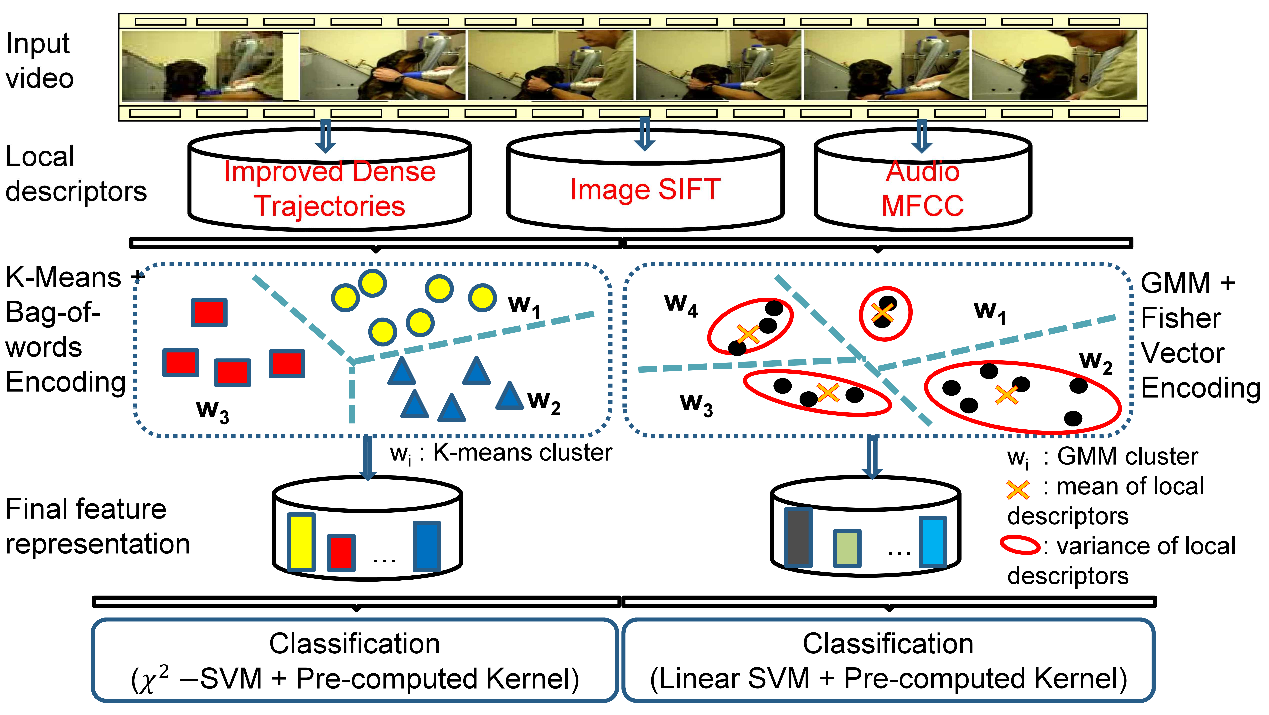
\includegraphics[width=1\textwidth]{framework.pdf}
	\caption{General MED framework}
	\label{med_framework}
\end{figure}




%*******************************************************************************
%*********************************** First Chapter *****************************
%*******************************************************************************

\chapter{Event Detection Using Segment-based Feature Representation}  %Title of the First Chapter
\label{chapter3}
%\setlength{\epigraphrule}{0pt}
\epigraph{\textit{Concentrate all your thoughts upon the work at hand. The sun's rays do not burn until brought to a focus.}}{ -- Alexander Graham Bell}

\ifpdf
    \graphicspath{{Chapter3/Figs/Raster/}{Chapter3/Figs/PDF/}{Chapter3/Figs/}}
\else
    \graphicspath{{Chapter3/Figs/Vector/}{Chapter3/Figs/}}
\fi


\section{Introduction}
\label{introduction:1}
Multimedia Event Detection (MED) is a challenging task in TREC Video Retrieval Evaluation (TRECVID)\footnote{http://trecvid.nist.gov/}. The task is defined as follow: given a collection of test videos and a list of test events, indicate whether each of the test events is present in each of the test videos. The aim of MED is to develop systems that can automatically find video containing any event of interest, assuming only a limited number of training exemplars are given.

%\begin{figure}
%	\centering
%	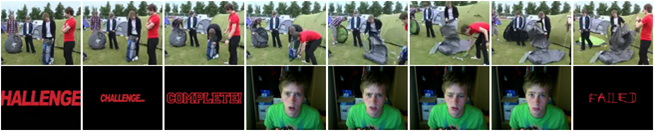
\includegraphics[width=1\textwidth]{teaser_image.eps}
%	\caption{(a) Example video for "making a sandwich" event: the related segment appears after a self-cam segment (unrelated); (b) example video for "grooming an animal" event: related segment is sandwiched between two unrelated segments. This kind of video is popular in realistic video datasets like MED. The frames with a red outlined box are examples of the extracted keyframes when using a keyframe-based approach, which suffers from both noise and missed extraction.}
%	\label{teaser_image}
%\end{figure}


The need for such MED systems is rising because a massive number of videos are produced every day. For example, more than 3 million hours of video are uploaded and over 3 billion hours of video are watched each month on YouTube\footnote{http://www.youtube.com/t/press\_statistics}, the most popular video sharing website. What is needed are the tools for automatically processing the video content and looking for the presence of a complex event in such unconstrained capturing videos. Automatic detection of complex events has great potential for many applications in the field of web video indexing and retrieval. In practice, a viewer may only want to watch goal scenes in a long football video, a housewife may need to search for videos that teach her how to make a cake, a handyman may look for how to repair an appliance, or a TV program manager may want to remove violent scenes in a film before it is aired.

However, detecting events in multimedia videos is a difficult task due to both the large content variation and uncontrolled capturing conditions. The video content is extremely diverse even in a same event class. The genres of video are also very varied, such as interviews, home videos, and tutorials. Moreover, the number of events is expected to be extensive for large scale processing. Each event, in its turn, can involve a number of objects and actions in a particular setting (indoors, outdoors, etc). Furthermore, multimedia videos are typically recorded under uncontrolled conditions such as different lighting, viewpoints, occlusions, complicated camera motions and cinematic effects. Therefore, it is very hard to model and detect of multimedia events.

The most straightforward approach toward building a large scale event detection system is using a bag-of-words (BoW) model \cite{Csurka04visualcategorization}. There are two types of BoW representations that are used for MED: BoW representation at the keyframe level and BoW representation at the video level. The first method is employed for still image features where the keyframes are often extracted at a fixed interval. The second method is employed for motion features where moving patterns from the entire video are extracted. These methods are respectively referred to as keyframe-based \cite{trecvid10:IBM,trecvid10:cuucf,DBLP:conf/trecvid/MatsuoN10} and video-based \cite{trecvid10:IBM,trecvid10:cuucf} in this chapter. Although these methods can obtain reasonable results, they all suffer from severe limitations. For the keyframe-based approach, temporal information is not incorporated in the model. Moreover, it is possible that important keyframes are missed extraction. Extracting more keyframes can tackle this problem but the scalability is also a problem for concern. On the other hand, the video-based approach is most likely to suffer from noise. We found that the video length is very different from video to video (even from videos of the same event class). In addition, the clues to determine an event may appear within a small segment of the entire video. Thus, comparing the BoW representation of two videos is unreliable because it may contain unrelated information. Figure \ref{c1_uncontrolled} illustrates these limitations for both approaches. 

In this chapter, we propose using a segment-based approach to overcome the limitations of both the keyframe-based and video-based approaches. The basic idea is to examine shorter segments instead of using the representative frames or entire video. We can reduce the amount of unrelated information in the final representation, while still benefiting from the temporal information by dividing a video into segments. In particular, we investigate two methods to cut a video into segments. The first method is called uniform sampling, where every segment has an equal length. We choose different segment lengths and use two types of sampling: non-overlapping and overlapping. The overlapped configuration is used to test the influence of dense segment sampling. The second method divides the video based on the shot boundary detection to take into account the boundary information of each segment. Once segments are extracted, we use dense trajectories, a state-of-the-art motion feature proposed by Wang \cite{wang:2011:inria-00583818:1}, for the feature extraction. After that, a BoW model is employed for the feature representation. The experimental results on TRECVID MED 2010 and TRECVID MED 2011 showed the improvement of the segment-based approach over the video-based approach. Moreover, a better performance can be obtained by using the overlapping sampling strategy. 

The rest of this chapter is organized as follows. Section \ref{relatedwork:1} introduces the related work. Section \ref{sec:1} gives an overview of the dense trajectory motion feature and our segment-based approach. The experimental setup including an introduction to the benchmark dataset and the evaluation method are presented in Section \ref{experimentalsetup}. Then, in Section \ref{experimentalresult}, we present and analyze our experimental results. Detailed discussions of these results are presented in Section \ref{discussion}. Finally, Section \ref{c3_conclusion} concludes this work with discussions on our future work. 

\section{Related Work}
\label{relatedwork:1}
Challenges began from TRECVID 2010\footnote{www.nist.gov/itl/iad/mig/med10.cfm}, and Multimedia Event Detection has drawn the attention of many researchers. Seven teams participated in the debut challenge and 19 teams participated the following year (MED 2011). Many MED systems have been built and different strategies have been used for the event detection system.

Columbia University (CU) team achieved the best result in TRECVID MED 2010. Their success greatly influenced later MED systems. In their paper \cite{trecvid10:cuucf}, they answered two important questions. The first question was, "What kind of feature is more effective for multimedia event detection?". The second one was, "Are features from different feature modalities (e.g., audio and visual) complementary for event detection?". Different kinds of features have been studied, such as SIFT \cite{Lowe:2004} for the image feature, STIP \cite{Laptev:2005:SIP} for the motion feature and MFCC (Mel-frequency cepstral coefficients \cite{Lee1998MFCC}) for the audio feature to answer the first question. In general, the STIP motion feature is the best single feature for MED. However, the system should combine strong complementary features from multiple modalities (both visual and audio) in order to achieve better results. 

The IBM team \cite{trecvid10:IBM} achieved the runner-up MED system in TRECVID 2010. They incorporated information from a wide range of static and dynamic visual features to build their baseline detection system. For the static features, they used the local SIFT \cite{Lowe:2004}, GIST \cite{DBLP:livaT01} descriptors and various global features such as Color Histogram, Color Correlogram, Color Moments, Wavelet Texture, etc. They used the STIP \cite{Laptev:2005:SIP} feature with a combined HOG-HOF \cite{Laptev08CVPR} descriptor for the dynamic feature.

The Nikon MED 2010 system \cite{DBLP:conf/trecvid/MatsuoN10} is also a remarkable system due to its simple but effective solution. They built a MED system based on the assumption that a small number of images in a given video contain enough information for event detection. Thus, they reduced the event detection task to the classification problem for a set of images, called keyframes. However, keyframe extraction is based on a scene cut detection technique \cite{Guimaraes:2003} that is less reliable in realistic videos. Moreover, the scene length is not consistent, which may affect the detection performance.

The BBN Viser system \cite{NIST-TRECVID11:BBN-DVMM} achieved the best performance at TRECVID MED 2011. Their success confirmed the effectiveness of the multiple modalities approach for multimedia event detection. In their work, they further investigated the performance of the appearance features (e.g., SIFT \cite{Lowe:2004}), color feature (e.g. RGB-SIFT \cite{vandeSandeTPAMI2010}), and motion (e.g., STIP \cite{Laptev:2005:SIP}), and also MFCC \cite{Lee1998MFCC} based audio features. Different kinds of fusion strategies have been explored, from which the novel non-parametric fusion strategy based on a video specific weighted average fusion has shown promising results.

In general, most systems used the multiple modalities approach to exploit different visual cues to build their baseline detection systems. Static image characteristics are extracted from frames within provided videos. Colombia University's results \cite{trecvid10:cuucf} suggest that methods for exploiting semantic content from web images, such as \cite{duan2012exploiting} and \cite{trecvid10:cuucf}, are not effective for multimedia event detection. For motion characteristics, most systems employed the popular STIP proposed by Laptev in \cite{Laptev:2005:SIP} for detecting complex actions. Other systems also took into account the HOG3D \cite{Klaser08BMVC} and MoSIFT \cite{Chen_mosift} motion features. All these systems used a video-based approach for the motion features, i.e., the motion features are extracted from the entire video. IBM's MED system \cite{trecvid10:IBM} also applied the video-based approach but the video was downsampled to five frames per second. One drawback of this video-based approach is that it may encode unrelated information in the final video representation. In a long video, the event information may happen during a small segment, and the information from the other segments tends to be noisy. That is why it is important to localize the event segment (i.e., where the event happens). This problem has been thoroughly investigated by Yuan et. al. \cite{Yuan2011PAMI}. Yuan proposed using a spatio-temporal branch-and-bound search to quickly localize the volume where an action might happen. In \cite{xu2008video}, Xu proposed a method to find optimal frame alignment in the
temporal dimension to recognize events in broadcast news. In \cite{duan2012visual}, a transfer learning method is proposed to recognize simple action events. However, these works are not applicable for complex actions in multimedia event videos.

Different from other approaches, we use a segment-based approach for the event detection. We did not try to localize the event volume like Yuan in \cite{Yuan2011PAMI}. In a simpler way, we use a uniform sampling with different segment lengths for our evaluation. We also investigate the benefit of using the shot boundary detection technique in \cite{Guimaraes:2003} for dividing video into segments. Moreover, an overlapped segment sampling strategy is also considered for a denser sampling. To the best of our knowledge, no MED system has previously used this approach. We evaluate its performance using the dense trajectories motion feature that was recently proposed by Wang in \cite{wang:2011:inria-00583818:1}. The dense trajectories feature has achieved state-of-the-art performances for various video datasets, including challenging datasets like Youtube Action \cite{liu2009recognizing} and UCF Sports \cite{Rodriguez2008}. In TRECVID MED 2012, the dense trajectories feature was also widely used by top performance systems such as AXES \cite{oneata:hal-00746874}, and BBNVISER \cite{NIST-TRECVID12:BBN-DVMM}. We use the popular ``bag-of-words'' model in \cite{Csurka04visualcategorization} as our feature representation technique. Finally, we use a Support Vector Machine (SVM) classifier for the training and testing steps. \index{segment-based}

\section{Dense Trajectories and Segment-based Approach}
\label{sec:1}
We introduce the dense trajectory motion feature proposed by Wang in \cite{wang:2011:inria-00583818:1} in this section. We additionally briefly review the trajectory extraction and description method. A detailed calculation of all the related feature descriptors, especially for Motion Boundary Histogram, is also presented. Our segment-based approach for motion features is introduced at the end of this section.

\subsection{Dense Trajectories} \index{dense trajectories}
\label{subsec:1}
Trajectories are obtained by tracking the densely sampled points using the optical flow fields. First, the feature points are sampled on a grid with a step size of 5 pixels and at multiple scales spaced by a factor of 1/$\sqrt{2}$. Then, the feature points are separately tracked in each scale. Each point $P_{t} = (x_{t}, y_{t})$ at frame \textit{t} is tracked to the next frame \textit{t+1} by using median filtering in a dense optical flow field $\omega$ = ($u_{t}$, $v_{t}$):
\begin{equation}
P_{t+1}=(x_{t+1}, y_{t+1})=(x_{t},y_{t}) + (M*\omega)|_{(\bar{x}_{t},\bar{y}_{t})},
\end{equation}
where \textit{M} is the median filter, and $(\bar{x}_{t},\bar{y}_{t})$ is the rounded position of $(x_{t}, y_{t})$.

After extracting a trajectory, two kinds of feature descriptors are adopted: a trajectory shape descriptor and a trajectory-aligned descriptor.

\textit{Trajectory shape descriptor:} The trajectory shape descriptor is the simplest one for representing an extracted trajectory. It is defined based on the displacement vectors. Given a trajectory of length L, its shape is described by the sequence S = ($\Delta P_{t}$ ,..., $\Delta P_{t+L-1}$), where $\Delta P_{t}$ = $P_{t+1} - P_{t}$ = ($x_{t+1} - x_{t}$, $y_{t+1} - y_{t}$). The resulting vector is then normalized by the sum of the magnitudes of the displacement vectors:
\begin{equation}
S'=\dfrac{(\Delta P_{t},...,\Delta P_{t+L-1})}{\sum_{j=t}^{t+L-1} \|\Delta P_{j}\|}
\end{equation}
\textit{Trajectory-aligned descriptor:} More complex descriptors can be computed within a space-time volume around the trajectory. The size of the volume is NxN spatial pixels and L temporal frames. This volume is further divided into a $n_{\sigma}$ x $n_{\sigma}$ x $n_{\tau}$ grid to encode the spatial-temporal information between the features. The default settings for these parameters are N = 32 pixels, L = 15 frames, $n_{\sigma}$ = 2, and $n_{\tau}$ = 3. The features are separately calculated and aggregated in each region. Finally, the features in all regions are concatenated to form a single representation for the trajectory. Three kinds of descriptors have been employed for representing trajectory following this design: The Histogram of Oriented Gradient (HOG), which was proposed by Dalal et al. in \cite{DBLP:DalalT05} for object detection, The Histogram of Optical Flow (HOF), which was used by Laptev in \cite{Laptev08CVPR} for human action recognition, and the Motion Boundary Histogram (MBH). The MBH descriptor was also proposed by Dalal et al.~\cite{Dalal06ECCV} for human detection, where the derivatives are computed separately for the horizontal and vertical components of the optical flow $I_{\omega}$ = ($I_{x}$, $I_{y}$). The spatial derivatives are computed for each component of the optical flow field $I_{x}$ and $I_{y}$ independently. After that, the orientation information is quantized into histogram, similarly to that for the HOG descriptor (8-bin histogram for each component). Finally, these two histograms are normalized separately with the $L_{2}$ norm and concatenated together to form the final representation. Since the MBH represents the gradient of the optical flow, constant motion information is suppressed and only the information concerning the changes in the flow field (i.e., motion boundaries) is kept.

According to the author \cite{wang:2011:inria-00583818:1}, the MBH descriptor is the best feature descriptor for dense trajectories. One interesting property of the MBH is that it can cancel out camera motion. That is why it shows significant improvement on realistic action recognition dataset compared to other trajectory descriptors. We only use the MBH descriptor in this study to test the performance of our proposed segment-based method.

\subsection{Segment-based Approach for Motion Feature}
\label{subsec:4}
\begin{figure}
	\centering
	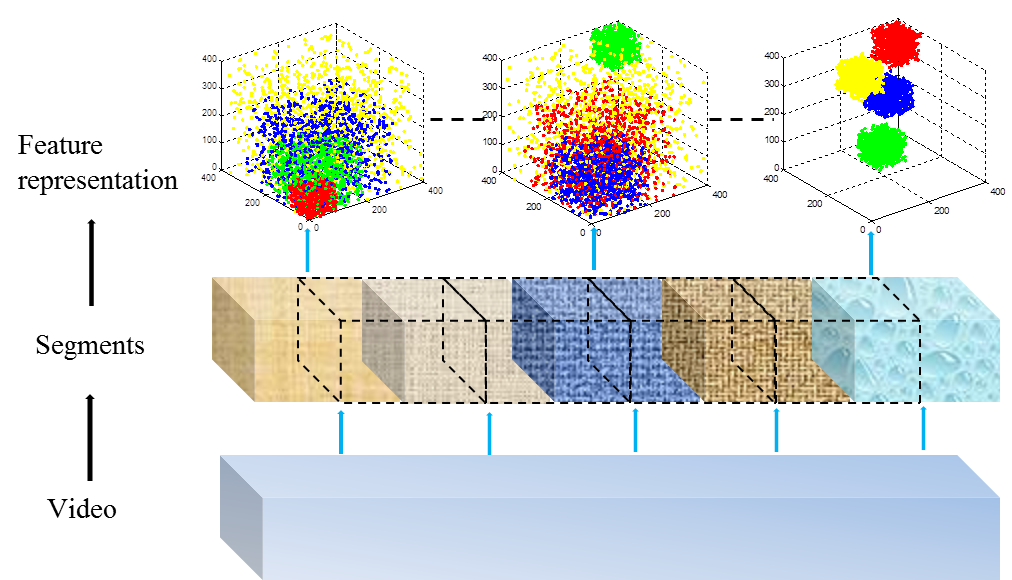
\includegraphics[width=1\textwidth]{segment_based.eps}
	\caption{Illustration of our segment-based approach. The original video is divided into segments by using non-overlapping and overlapping sampling (overlapped segment examples are drawn in dashes). After that, the feature representation is separately calculated for each segment. This figure is best viewed in color.}
	\label{segmentbased}
\end{figure}

Our proposed segment-based approach is as follows. At first, the video is divided into fixed length segments. We choose different segment lengths to pick the optimal one. In particular, we choose segment lengths of 30, 60, 90, 120, 200 and 400 seconds. The lengths of 120 and 60 seconds are respectively close to the mean (115 s) and geometric mean (72 s) length of the training dataset. The geometric mean value is also considered because it can eliminate the influence of outline cases, i.e., videos of exceptionally long durations. After that, the dense trajectory features are extracted from the entire segment. A "bag-of-words" approach is used to generate the final representation for each segment from the raw trajectory features (Fig. \ref{segmentbased}).

For the previous segment-based approach, a video is divided into continuous segments. This means information about the semantic boundary of a segment is not taken into account. However, this information is important because it keeps the semantic meaning of each segment. The simplest way to overcome this drawback is to use a denser sampling such as the overlapped segments. We use an overlapping strategy for the same segment length as in the non-overlapping experiments. In practice, we use uniform segment sampling with 50\% of overlapping. This means the number of segments will be doubled for each overlapping experiment.

Another way to extract segments with boundary information is to employ a shot boundary detection technique. For a fast implementation, we use the algorithm proposed in \cite{Guimaraes:2003}. This technique is also used in the Nikon 2010 MED system \cite{DBLP:conf/trecvid/MatsuoN10}. Basically, at first, this method constructs a space-time image from the input video. We can sample points or calculate the color histogram for each frame to construct the space-time image. This will reduce the 2D frame image to the space dimension of the space-time image. The time dimension is the number of frames of the video. The Canny edge detection algorithm is used to detect the vertical lines after attaining the space-time image. Each detected vertical line is considered as a scene cut. The method in \cite{Guimaraes:2003} also proposed solutions for other kinds of scene transitions such as a fade or wide. However, from our previous study, this method showed poor results in these cases. Thus, we only adopted the scene cut detection algorithm. Each detected scene cut is considered a segment in our experiments. \index{shot boundary detection}

Our proposed segment-based approach is compared with the video-based one. Actually, when the segment length is long enough, it becomes the entire video. In that case, we can consider the video-based approach a special type of segment-based approach.
\section{Experimental Setup}
\label{experimentalsetup}
\subsection{Dataset}
\label{experimentalsetup:1}
We tested our method on TRECVID MED 2010 and TRECVID MED 2011 datasets. An event kit is provided with the definitions and textual descriptions for all the events for each dataset. The first dataset contains 3,468 videos, including 1,744 videos for training and 1,724 video clips for testing, containing a total of more than 110 video hours. In TRECVID MED 2010, there are 3 events classes: assembling a shelter, batting in a run, and making a cake. The TRECVID MED 2011 dataset defined the 15 event classes listed in Table \ref{med11}. The first five events (E001-E005) are used for training and validation and the last 10 events (E006-E015) are used for testing. It comprises of over 45,000 video clips for a total of 1,400 hours of video data. All the video clips are divided into three sets: event collection (2392 video clips), development collection (10198 video clips), and test collection (31,800 video clips). It is worth noting that these two datasets contain a major number of background video clips, i.e., video clips that do not belong to any event. The number of positive videos in the event collection is also listed in Table \ref{med11}.

% Table generated by Excel2LaTeX from sheet 'Sheet1'
\begin{table}[!h]
	\renewcommand{\arraystretch}{1.3}
	\centering
	\caption{List of events and its number of positive samples in event collection set of MED 2011 dataset.}
	\begin{tabular}{|c|l|c|}
		\toprule
		Event ID & Event Name & \#Pos videos \\
		\midrule
		E001  & Attempting a board trick & 173 \\
		\midrule
		E002  & Feeding an animal & 168 \\
		\midrule
		E003  & Landing a fish & 152 \\
		\midrule
		E004  & Wedding ceremony & 163 \\
		\midrule
		E005  & Working on a woodworking project & 159 \\
		\midrule
		E006  & Birthday party & 221 \\
		\midrule
		E007  & Changing a vehicle tire & 119 \\
		\midrule
		E008  & Flashmob gathering & 191 \\
		\midrule
		E009  & Getting a vehicle unstuck & 151 \\
		\midrule
		E010  & Grooming an animal & 143 \\
		\midrule
		E011  & Making a sandwich & 186 \\
		\midrule
		E012  & Parade & 171 \\
		\midrule
		E013  & Parkour & 134 \\
		\midrule
		E014  & Repairing an appliance & 137 \\
		\midrule
		E015  & Working on a sewing project & 124 \\
		\bottomrule
	\end{tabular}%
	\label{med11}%
\end{table}%

\subsection{Evaluation Method}
\label{experimentalsetup:2}
%
Figure \ref{framework} shows our evaluation framework for the motion features. We conducted experiments using the proposed segment-based approach and the video-based approach for comparison. We use the library published online by the author\footnote{http://lear.inrialpes.fr/people/wang/dense\_trajectories} to extract dense trajectory feature. The source code is customized for pipeline processing using only an MBH descriptor to save computing time but other parameters are set to default. Due to the large number of features produced when using the dense sampling strategy, we use the "bag-of-words" approach to generate the features for each segment. At first, we randomly select 1,000,000 dense trajectories for clustering to form a codebook of 4000 visual codewords. After that, the frequency histogram of the visual words is computed over the videos/segments to generate the final feature vector. We also adopt the soft assignment weighting scheme, which was initially proposed by Jiang in \cite{Jiang:2007:TOB}, to improve the performance of the ``bag-of-words'' approach.
\begin{figure}
	\centering
	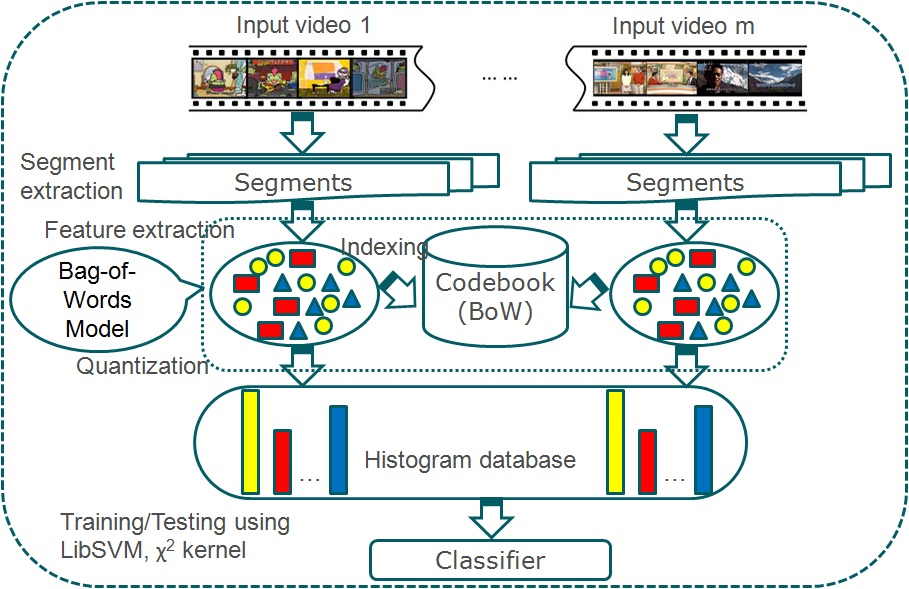
\includegraphics[width=1\textwidth]{baseline_framework.jpg}
	\caption{Evaluation framework for our baseline MED system}
	\label{framework}
\end{figure}

Once all the features are extracted, we use the popular Support Vector Machine (SVM) for the classification. In particular, we use the LibSVM library available online\footnote{http://www.csie.ntu.edu.tw/{\textasciitilde}cjlin/libsvm/} and adopt the one-vs.-rest scheme for multi-class classification. We annotate the data in the following way to prepare it for the classifier. All the videos/segments from positive videos are considered positive samples, and the remaining videos/segments (in the development set) are chosen as the negative samples. For testing purposes, we also use the LibSVM to predict the scores of the videos/segments in each testing video. The score of a video is defined as the largest score among its videos/segments. This score indicates how likely a video belongs to an event class.

\section{Experimental Result}
\label{experimentalresult}

\begin{table*}
	\renewcommand{\arraystretch}{1.3}
	\caption{Results on the MED 2010 dataset using non-overlapping sampling.}
	\label{t_med10_nonoverlapping}
	\centering
	\begin{tabular}{|l|cccccc|c|}
		\toprule
		Event/MAP & 30 s & 60 s & 90 s & 120 s & 200 s & 400 s & Late fusion \\
		\midrule
		\begin{tabular}[x]{@{}c@{}}Assembling\\a shelter\end{tabular} &0.4140&0.4511&0.4339&0.4457&0.4595&\textbf{0.4610}&0.4532
		%&0.353&0.533
		\\
		\midrule
		Batting in a run&0.7650&0.7852&0.7799&0.7553&0.7823&\textbf{0.7871}&0.7181
		%&0.787&0.873
		\\
		\midrule
		Making a cake&0.3596&0.3636&0.3433&0.3569&0.3058&0.3032&\textbf{0.3727}
		%&0.396&0.493
		\\
		\midrule
		All&0.5129&\textbf{0.5333}&0.5190&0.5193&0.5158&0.5171&0.5146
		
		%&0.512&0.633
		\\
		\bottomrule
	\end{tabular}
\end{table*}
This section presents the experimental results from using our proposed approach on the MED 2010 and MED 2011 dataset. We also present the results of combining various segment lengths using the late fusion technique. This is a simple fusion technique where the predicted score of each video is the average one of that video in all combined runs. We also report the performance of our baseline event detection system using the keyframe-based and video-based approach for comparison.  

All the experiments were performed on our grid computers. We utilized up to 252 cores for the parallel processing using Matlab codes. All the results are reported in terms of the Mean Average Precision (MAP). We calculate MAP using the TRECVID evaluation tool\footnote{http://www-nlpir.nist.gov/projects/trecvid/trecvid.tools/} from the final score of each video in the test set. The best performing feature is highlighted in bold for each event. 
\begin{table*}
	\renewcommand{\arraystretch}{1.3}
	\caption{Results on the MED 2010 dataset using overlapping sampling.}
	\label{t_med10_overlapping}
	\centering
	\begin{tabular}{|l|cccccc|c|}
		\toprule
		Event/MAP & 30 s & 60 s & 90 s & 120 s & 200 s & 400 s & Late fusion \\
		%\bfseries \begin{tabular}[c]{@{}c@{}} CU\\(SIFT)\end{tabular}&
		%\bfseries \begin{tabular}[c]{@{}c@{}}CU (STIP,\\SIFT,\\MFCC)\end{tabular}\\
		\midrule
	\begin{tabular}[x]{@{}c@{}}Assembling\\a shelter\end{tabular} &0.4177&\textbf{0.4781}&0.4617&0.4614&0.4601&0.4682&0.4486
		\\
		\midrule
		Batting in a run&0.7727&0.7918&\textbf{0.7975}&0.7886&0.7893&0.7756&0.7691
		\\
		\midrule
		Making a cake&0.4083&0.3819&0.3155&0.3415&0.3464&0.3239&\textbf{0.4232}
		\\
		\midrule
		All&0.5329&\textbf{0.5506}&0.5249&0.5305&0.5319&0.5226&0.5470
		%&0.512&0.633
		\\
		\bottomrule
	\end{tabular}
\end{table*}
\begin{figure}
	\centering
	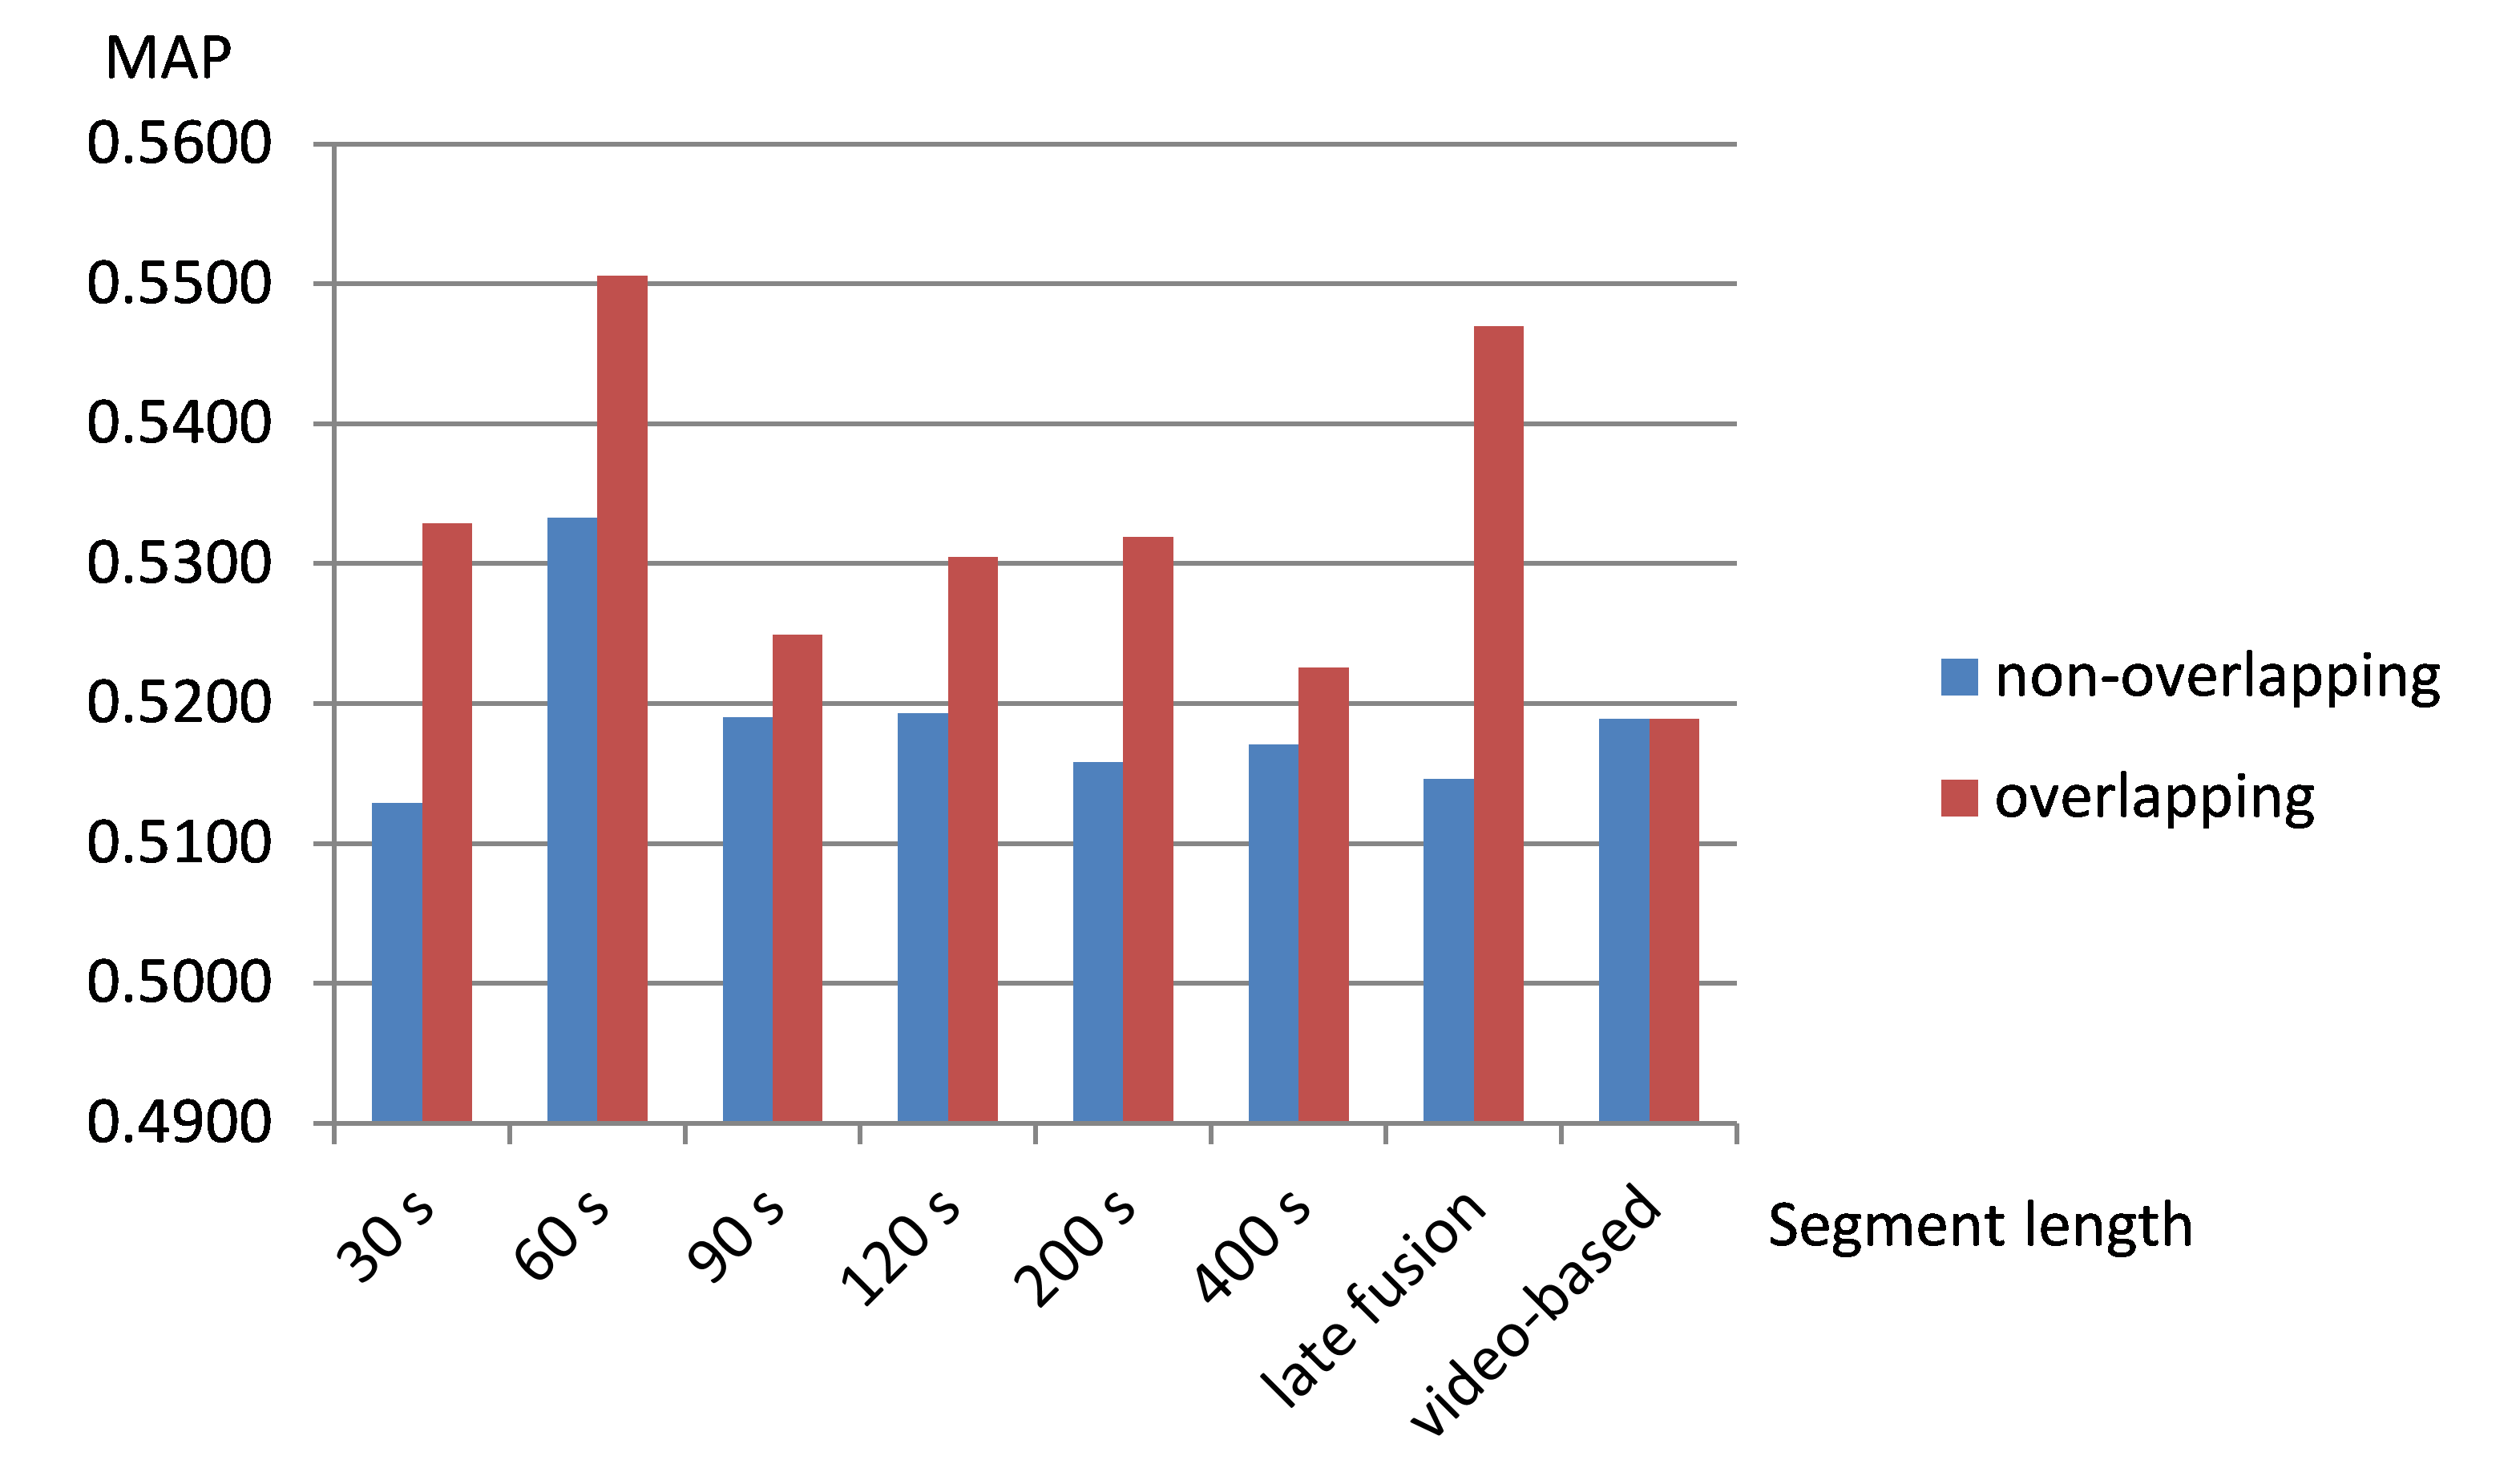
\includegraphics[width=1\textwidth]{med10_result.eps}
	\caption{Results from using segment-based approach with non-overlapping and overlapping sampling on MED 2010. In all cases, the overlapping sampling performs the best}
	\label{f_med10_result}
\end{figure}

\subsection{On TRECVID MED 2010}
\subsubsection{Non-overlapping and overlapping sampling}\label{experimentalresult:1} Table \ref{t_med10_nonoverlapping} lists the results from our segment-based approach when using a non-overlapping sampling strategy. These results show that the performance is rather sensitive to the segment length and it is also event-dependent. For example, the detection results of the first event, ``assembling a shelter'', are better when the segment length is increased. On the other hand, the ``making a cake'' event tends to be more localized, i.e. the shorter the segment, the better the performance. The performance of the ``batting in a run'' event is quite stable when segment length is longer than 60 s. However, it is decreased 2\% at 30 s. This suggests that shorter lengths can harm the performance. In general, the performance of a 60-s segment is the best. This length is also around the geometric mean length of the training set. Thus, we got peak results for segment length around geometric mean point. 

We further investigated the performance of a denser segment sampling, i.e., an overlapping sampling strategy. Interestingly, the MAP score in Table \ref{t_med10_overlapping} is consistently increased for each event compared to the results without using overlapped segments. Figure \ref{f_med10_result} shows a detailed comparison between the two strategies in terms of the over-all performance. We again found that the performance with a segment length around the geometric mean length (60 s) was the best. We also combined the performances of all the segment lengths using late fusion and the results are listed in the last column of Tables \ref{t_med10_nonoverlapping} and \ref{t_med10_overlapping}. The late fusion strategy can benefit the ``making a cake'' event, but it decreased the performances of the remaining events. The overall performance is lower than the best one.
%The performance gain means that denser segment sampling is better. In another words, not only the length of the segment is %important, the location of the segment is also important. This observation lead us to another experiment: using shot boundary %information for choosing segments.

\subsubsection{Segment sampling based on shot boundary detection}
\label{experimentalresult:3}
% For tables use
\begin{table*}
	\renewcommand{\arraystretch}{1.3}
	\caption{Comparison of different segment-based approaches with the video-based approach on the MED 2010 dataset.}
	\label{t_med10_comparison}
	\centering
	% For LaTeX tables use
	\begin{tabular}{|l|ccc|c|c|}
		\toprule
		Event/MAP & \begin{tabular}[x]{@{}c@{}}Best\\non-overlapping\end{tabular}& Best overlapping & SBD segments & Video-based\\
		\midrule
		Assembling shelter & 0.4511 & 0.4781& 0.4284  & \textbf{0.4911} \\
		\midrule
		Batting in a run & 0.7852 &\textbf{0.7918}& 0.7866 & 0.7902 \\
		\midrule
		Making a cake & 0.3636 & \textbf{0.3819} & 0.1918 & 0.2755 \\
		\midrule
		All & 0.5333 & \textbf{0.5506} & 0.4689 & 0.5189 \\
		\bottomrule
	\end{tabular}
\end{table*}

The second column in Table \ref{t_med10_comparison} shows the performance when shot boundary detection is used to extract segments. Unexpectedly, the performance is quite low even when compared with the video-based approach (listed in the last column). There are two possible reasons for this low level of performance: (1) The shot boundary detection technique is inaccurate when used on uncontrolled capturing videos; (2) the shot units may not contain enough information to determine an event. The second reason suggests that combining multiple shots to form a segment may improve the performance. Thus, we have conducted a segment-based experiment based on this observation using segments extracted from multiple shots. However, we did not see any significant improvement. Thus, the first reason is why this experiment had poor result.

We also included the best results from the segment-based experiments using non-overlapping and overlapping sampling in Table \ref{t_med10_comparison} for comparison. In general, our segment-based approach outperforms the video-based approach by more than 3\% in terms of MAP. We did not conduct a keyframe-based experiment because we learned that it is inefficient compared to the video-based approach.

\subsection{On TRECVID MED 2011}

\begin{figure}
	\centering
	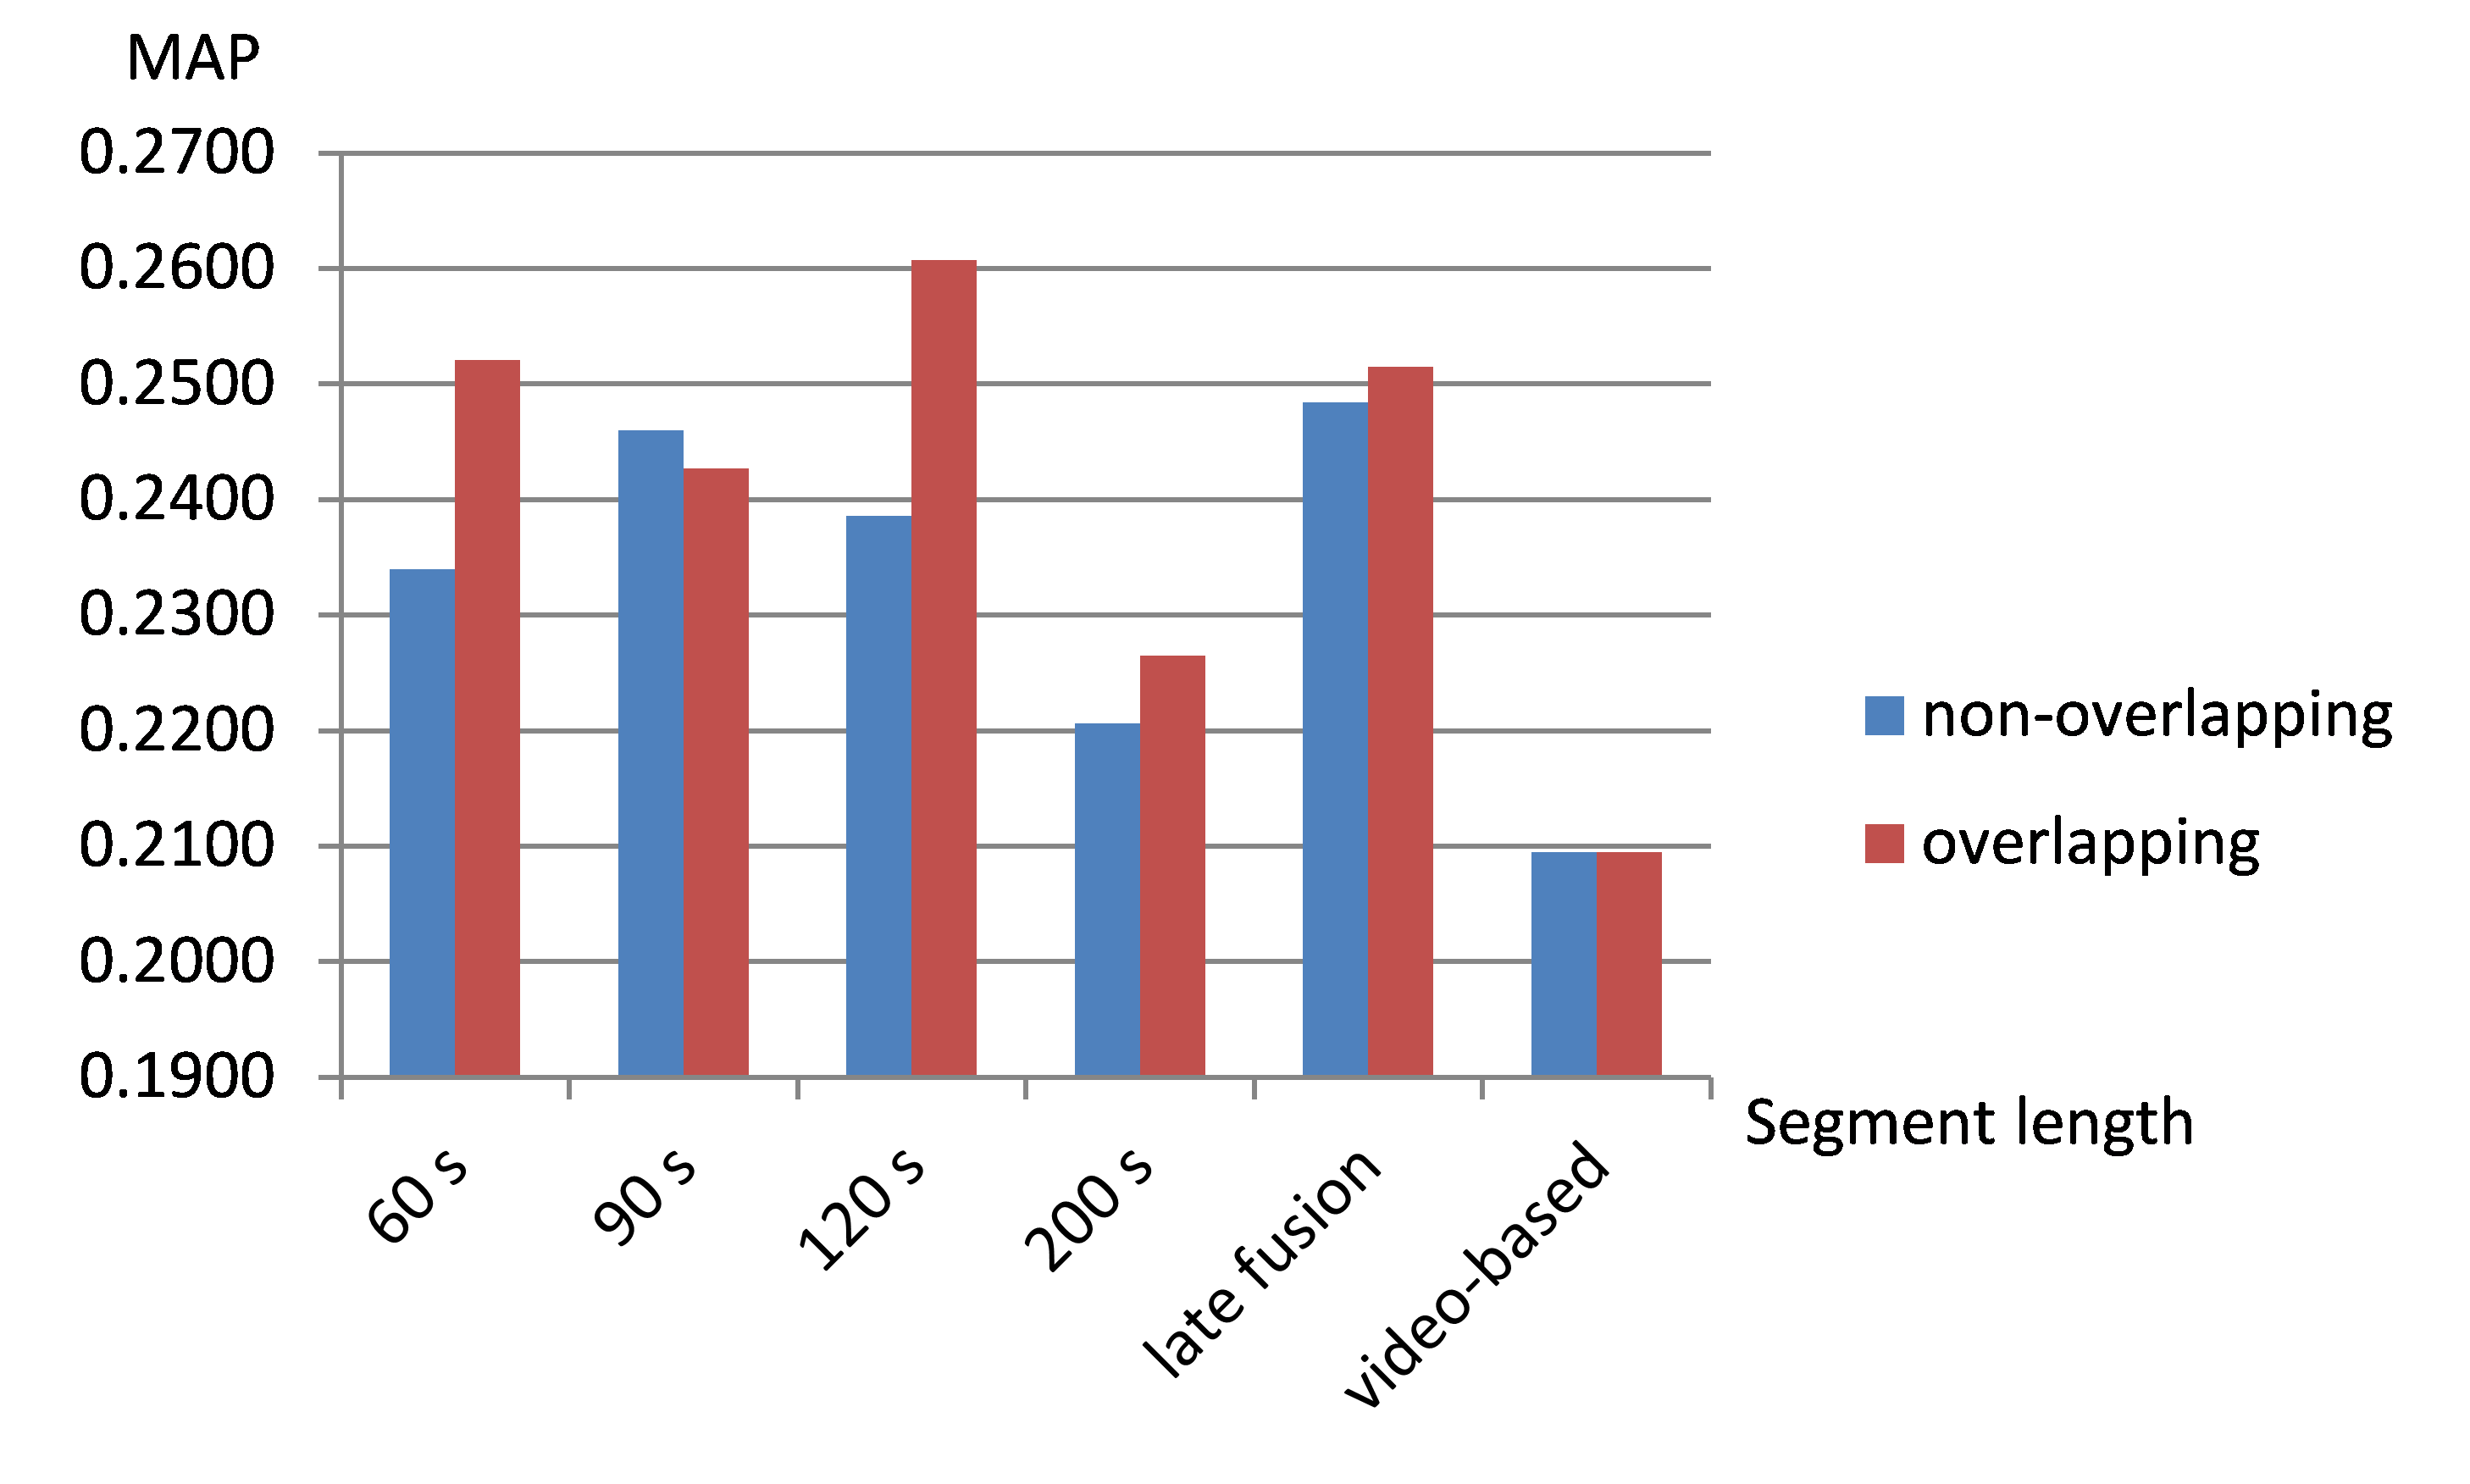
\includegraphics[width=1\textwidth]{med11_result.eps}
	\caption{Results from using segment-based approach with non-overlapping and overlapping sampling on MED 2011. In most cases, the overlapping sampling performs the best.}
	\label{f_med11_result}
\end{figure}

We conducted the same segment-based experiments on MED 2011. For both the non-overlapping and overlapping experiments, we chose segment lengths of 60, 90, 120, and 200 seconds and compare them with the video-based approach. A late fusion strategy is also used to combine the performances of different segment lengths. We did not conduct a shot boundary detection experiment because we showed that it is inefficient. Tables \ref{t_med11_nonoverlapping} and \ref{t_med11_overlapping} list the performances of each event for non-overlapping and overlapping experiment, respectively. Figure \ref{f_med11_result} shows a better view for comparing the overall performance. The result from using video-based approach, which is 0.2095 MAP, is also included for comparison. In most cases, the overlapping sampling had better results than the non-overlapping sampling. In all cases, the segment-based approach also outperforms the video-based approach. The best improvement was about 5\%, which was obtained at 120 s using an overlapping sampling. The late fusion run also confirms its effectiveness for some events, such as ``Flash-mob gathering'' and ``Working on a sewing project''.

% Table generated by Excel2LaTeX from sheet 'new-exp'
\begin{table}[!h]
	\renewcommand{\arraystretch}{1.3}
	\centering
	\caption{Results on the MED 2011 dataset using non-overlapping sampling.}
	\label{t_med11_nonoverlapping}
	\begin{tabular}{|c|c|c|c|c|c|}
		
		\toprule
		\begin{tabular}[x]{@{}c@{}}Event/\\MAP\end{tabular} & 60 s   & 90 s   & 120 s   & 200 s  & \begin{tabular}[x]{@{}c@{}}Late\\fusion\end{tabular} \\
		
		\midrule
		E006&0.1060&\textbf{0.1277}&0.1162&0.1005&0.1217\\
		\midrule
		E007&0.1003&\textbf{0.1521}&0.1461&0.0539&0.1419\\
		\midrule
		E008&0.4811&0.4923&0.4840&0.4508&\textbf{0.4975}\\
		\midrule
		E009&0.2077&0.2072&0.1962&0.1860&\textbf{0.2145}\\
		\midrule
		E010&0.0794&\textbf{0.0916}&0.0486&0.0854&0.0771\\
		\midrule
		E011&\textbf{0.0943}&0.0698&0.0903&0.0703&0.0805\\
		\midrule
		E012&0.3061&0.3560&0.3052&\textbf{0.3639}&0.3309\\
		\midrule
		E013&0.5974&0.6030&0.5861&0.5941&\textbf{0.6033}\\
		\midrule
		E014&0.2307&0.2008&\textbf{0.2772}&0.1723&0.2585\\
		\midrule
		E015&0.1364&\textbf{0.1599}&0.1357&0.1284&0.1583\\
		\midrule
		All&0.2340&0.2460&0.2386&0.2206&\textbf{0.2484}\\
		\bottomrule
		
	\end{tabular}%
\end{table}%

\begin{figure}
	\centering
	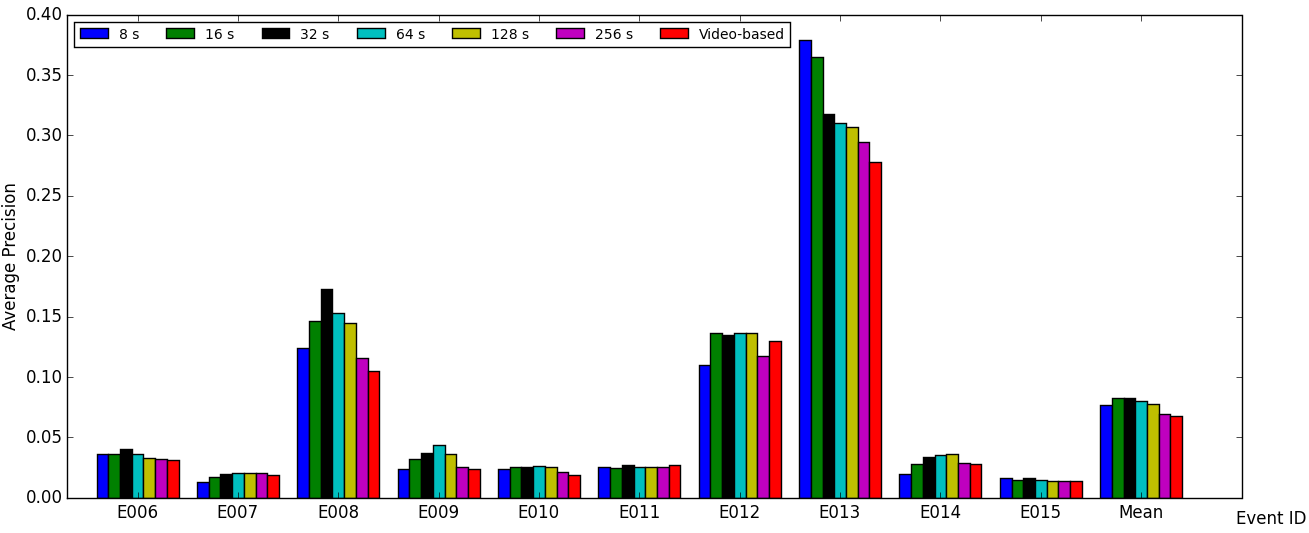
\includegraphics[width=1.1\textwidth]{sb_linear_max.png}
	\caption{Results from using segment-based approach with non-overlapping on the updated MED 2011 dataset.}
	\label{f_med11_update}
\end{figure}

The updated MED 2011 dataset has less number of training videos (See Table \ref{c2_exp_dataset}). We also verify the effectiveness of our approach on this dataset. We conduct experiments at different segment lengths including  8 s, 16 s, 32 s, 64 s, 128 s and 256 s. The overall performance is shown in the last group of Fig. \ref{f_med11_update}.

% Table generated by Excel2LaTeX from sheet 'new-exp'
\begin{table}[!h]
	\renewcommand{\arraystretch}{1.3}
	\centering
	\caption{Results on the MED 2011 dataset using overlapping sampling.}
	\label{t_med11_overlapping}  
	\begin{tabular}{|c|c|c|c|c|c|}
		
		\toprule
		\begin{tabular}[x]{@{}c@{}}Event/\\MAP\end{tabular} & 60 s   & 90 s   & 120 s   & 200 s  & \begin{tabular}[x]{@{}c@{}}Late\\fusion\end{tabular} \\
		
		\midrule  
		E006  & 0.1074 & 0.1069 & \textbf{0.115}1 & 0.1010 & 0.1086  \\
		\midrule  
		E007  & 0.1570 & \textbf{0.1733} & 0.1552 & 0.1466 & 0.1610 \\
		\midrule  
		E008  & 0.4788 & 0.4767 & 0.4969 & 0.4620 & \textbf{0.4903}\\
		\midrule  
		E009  & 0.1830 & 0.1999 & \textbf{0.2160} & 0.1972 & 0.1954 \\
		\midrule  
		E010  & \textbf{0.1150} & 0.0851 & 0.1008 & 0.0746 & 0.1108 \\
		\midrule  
		E011  & 0.0602 & 0.0885 & \textbf{0.1591} & 0.0779 & 0.0819\\
		\midrule  
		E012  & \textbf{0.3674} & 0.3129 & 0.3150 & 0.3075 & 0.3293\\
		\midrule  
		E013  & 0.6025 & 0.5893 & \textbf{0.6188} & 0.5675 & 0.5872\\
		\midrule  
		E014  & 0.2718 & 0.2487 & \textbf{0.2744} & 0.2095 & 0.2706\\
		\midrule  
		E015  & 0.1777 & 0.1459 & 0.1562 & 0.1214 & \textbf{0.1795} \\
		\midrule  
		All   & 0.2521 & 0.2427 & \textbf{0.2607} & 0.2265 & 0.2515 \\
		\bottomrule    
		
	\end{tabular}%
\end{table}%



\section{Discussion}
\label{discussion}
\subsection{Optimal Segment Length} 
It is true that the lengths of the event segments are quite different, even for the same events. Therefore, the fixed length video segments are obviously not the optimal solution to describe the events. However, compared to the video-based approach, as shown in our experiments on the datasets of TRECVID MED 2010 and TRECVID MED 2011, the segment-based approach using overlapping strategy for extracting segments consistently outperforms.

It is ideal if the boundary of the event segment can be determined. However, this localization problem is difficult. The straightforward way to tackle this problem is extracting segments based on shot boundary information. This solution is reasonable because the event might be localized in certain shots. However, we obtained unexpected results due to the unreliability of shot boundary detection in uncontrolled video dataset and the event segment might span to several shots.

The method described in \cite{DBLP:conf/eccv/JiangYY12} suggests another approach to divide a video into segments. Instead of learning a randomized spatial partition for images, we can learn a randomized temporal partition for videos. However, this approach needs sufficient positive training samples while MED datasets have a small number of positive samples with large variation. On the other hand, it is also not scalable because learning and testing the best randomized pattern is time-consuming. Therefore, the fixed-length approach is quite simple but still effective.

Supposed the segment length is fixed, what is the optimal segment length for event detection? This is a difficult question and the answer depends on the dataset. The results of late fusion are quite close to the peak performance of each experiment. This suggests a methodical way to choose the optimal segment length, i.e., combining multiple lengths together (which is similar to \cite{DBLP:conf/eccv/JiangYY12}). However, to achieve the scalability, we should reduce the number of combined lengths as much as possible. From the experimental results on both the MED 2010 and MED 2011 dataset, we observed that with segment length from 60 s to 120 s, the performance is rather stable and close to the peak result. Interestingly, this range is approximate to the range from the geometric mean length to (arithmetic) mean length of the training sets. We also combined multiple segment lengths together using late fusion with equal weights for all segment lengths for comparison. There are two combined runs: one for segment lengths from 60 s to 120 s and the other is for all segment lengths. The result obtained when combining segment lengths from 60 s to 120 s is equivalent to the result obtained when combining all lengths, as shown in Table \ref{t_med11_comparison}. Therefore, based on this observation, we can choose the first combined run as an efficient way for solving the optimal segment length problem of the proposed segment-based approach on other datasets.

\begin{table*}
	\renewcommand{\arraystretch}{1.3}
	\newcolumntype{H}{>{\setbox0=\hbox\bgroup}c<{\egroup}@{}}
	\caption{Comparison of different segment-based approaches with the video-based approach on the MED 2011 dataset.}
	\label{t_med11_comparison}
	\centering
	\begin{tabular}{|c|c|c|c|c|}
		\hline
		\multirow{3}[4]{*}{Event/MAP} & \multicolumn{3}{|c|}{Non-overlapping sampling} &  \multirow{3}[4]{*}{Video-based} \\ 
		\cline{2-4}
		& \begin{tabular}[x]{@{}c@{}}Best\\(at 90 s) \end{tabular}
		& \begin{tabular}[x]{@{}c@{}}Late fusion\\(all lengths) \end{tabular}
		& \begin{tabular}[x]{@{}c@{}}Late fusion\\(60, 90, 120 s) \end{tabular} & \\ \hline
		
		E006  & \multicolumn{1}{|c|}{\textbf{0.1277}} & 0.1217 & 0.1244 & 0.0959 \\ \hline
		
		E007  & \multicolumn{1}{|c|}{0.1521} & 0.1419 & \multicolumn{1}{|c|}{0.1369} & 0.1303 \\	\hline
		E008  & \multicolumn{1}{|c|}{0.4923} & \textbf{0.4975} & \multicolumn{1}{|c|}{0.4973} & 0.4766 \\	\hline
		E009  & \multicolumn{1}{|c|}{0.2072} & 0.2145 & \multicolumn{1}{|c|}{0.2064} & 0.0943 \\	\hline
		E010  & \multicolumn{1}{|c|}{0.0916} & 0.0771 & \multicolumn{1}{|c|}{0.0753} & 0.1020 \\	\hline
		E011  & \multicolumn{1}{|c|}{0.0698} & 0.0805 & \multicolumn{1}{|c|}{0.0813} & 0.0609 \\	\hline
		E012  & \multicolumn{1}{|c|}{\textbf{0.3560}} & 0.3309 & \multicolumn{1}{|c|}{0.3277} & 0.2858 \\	\hline
		E013  & \multicolumn{1}{|c|}{0.6030} & 0.6033 & \multicolumn{1}{|c|}{0.6096} & 0.5385 \\	\hline
		E014  & \multicolumn{1}{|c|}{0.2008} & 0.2585 & \multicolumn{1}{|c|}{0.2579} & 0.2138 \\	\hline
		E015  & \multicolumn{1}{|c|}{0.1599} & 0.1583 & \multicolumn{1}{|c|}{0.1622} & 0.0964 \\	\hline
		All   & \multicolumn{1}{|c|}{0.2460} & 0.2484 & \multicolumn{1}{|c|}{0.2479} & 0.2095 \\	\hline
		
	\end{tabular}%
	\label{tab:addlabel}%
\end{table*}%



\begin{table*}
	\renewcommand{\arraystretch}{1.3}
	\caption{Comparison of different segment-based approaches with the video-based approach on the MED 2011 dataset.}
	\label{t_med11_comparison}
	\centering
	\begin{tabular}{|c|c|c|c|c|}
		\toprule
		\multirow{3}[4]{*}{Event/MAP} & 
		 \multicolumn{3}{|c|}{Overlapping sampling} & \multirow{3}[4]{*}{Video-based} \\ 
		\cline{2-4}
		& \begin{tabular}[x]{@{}c@{}}Best\\(at 120 s) \end{tabular}
		& \begin{tabular}[x]{@{}c@{}}Late fusion\\(all lengths) \end{tabular}
		& \begin{tabular}[x]{@{}c@{}}Late fusion\\(60, 90, 120 s) \end{tabular} &  \\ \midrule
		E006  & 0.1151 & 0.1086 & \multicolumn{1}{|c|}{0.1083} & 0.0959 \\ \midrule
		
		E007  & 0.1552 & 0.1610 & \multicolumn{1}{|c|}{\textbf{0.1616}} & 0.1303 \\	\midrule
		E008  & 0.4969 & 0.4903 & \multicolumn{1}{|c|}{0.4871} & 0.4766 \\	\midrule
		E009  & \textbf{0.2160} & 0.1954 & \multicolumn{1}{|c|}{0.1958} & 0.0943 \\	\midrule
		E010  & 0.1008 & 0.1108 & \multicolumn{1}{|c|}{\textbf{0.1109}} & 0.1020 \\	\midrule
		E011  & \textbf{0.1591} & 0.0819 & \multicolumn{1}{|c|}{0.0845} & 0.0609 \\	\midrule
		E012  & 0.3150 & 0.3293 & \multicolumn{1}{|c|}{0.3341} & 0.2858 \\	\midrule
		E013  & \textbf{0.6188} & 0.5872 & \multicolumn{1}{|c|}{0.5910} & 0.5385 \\	\midrule
		E014  & \textbf{0.2744} & 0.2706 & \multicolumn{1}{|c|}{0.2694} & 0.2138 \\	\midrule
		E015  & 0.1562 & 0.1795 & \multicolumn{1}{|c|}{\textbf{0.1795}} & 0.0964 \\	\midrule
		All   & \textbf{0.2607} & 0.2515 & \multicolumn{1}{|c|}{0.2522} & 0.2095 \\	\bottomrule
		
	\end{tabular}%
	\label{tab:addlabel2}%
\end{table*}%

\subsection{Scalability} For scalability, we discuss the storage and computation costs of our experiments. At first, our system does not consume a lot of disk storage because we only store the final representation of the videos or segments, not the raw features. We calculated the BoW features directly from the raw feature outputs using a pipeline reading technique. One drawback is that this technique requires a lot of memories. However, we handled this problem by encoding the raw features into smaller chunks and aggregating them to generate the final representation. By this way, we can manage the mount of memory usage.

In our framework, the most time-consuming steps are the feature extraction and representation (using the bag-of-words model). It is worth noting that the computation time for one video is independent of the segment length, which means our segment-based approach has the same computational cost as the video-based approach. On the other hand, when we do experiments at the segment level, we will have more training and testing samples than that in the video-based approach. Thus, it will cost more in time to train and test using the segment-based approach. However, this cost is relatively small compared with the feature extraction and representation cost. For example, when using a grid computer with 252 cores, it took us about 10 hours to generate the feature representation for each segment-based experiment on MED 2010 dataset. In the mean time, we used one-core processor for the training and testing, but it only took about 4-8 hours for the training and 2-4 hours for the testing on each event. For the MED 2011 dataset, the computational cost was around 13 times bigger than the MED 2010 (linearly to the number of videos it contains).

\section{Conclusion}
\label{c3_conclusion}
We proposed using the segment-based approach for multimedia event detection in this work. We evaluated our approach by using the state-of-the-art dense trajectories motion feature on the TRECVID MED 2010 and TRECVID MED 2011 datasets. Our proposed segment-based approach outperforms the video-based approach in most cases when using a simple non-overlapping sampling strategy. More interestingly, the results are significantly improved when we using the segment-based approach with an overlapping sampling strategy. Therefore, the effectiveness of our methods on realistic datasets like MEDs is confirmed.

A segment-based approach with an overlapping sampling strategy shows promising results. This suggests the importance of segment localization on the MED performance. Suppose the segment length is fixed, we are interested in determining which segment is the best representative for an event. In this study, we also observed that the detection performance is quite sensitive to the segment-length and it depends on the dataset. The results obtained from the late fusion strategy is quite stable and close the peak performance. This suggests a methodical way to generalize the segment-based approach to other datasets. However, this method is not scalable because it requires a lot of computation costs. Therefore, learning an optimal segment length for each event can be beneficial for an event detection system. This is also an interesting direction for our future study.


%*******************************************************************************
%****************************** Second Chapter *********************************
%*******************************************************************************

\chapter{Event Detection Using Sum-max Feature Aggregation}
\label{chapter4}
\epigraph{\textit{A clay pot sitting in the sun will always be a clay pot. It has to go through the white heat of the furnace to become porcelain.}}{ -- Mildred W. Struven}

\ifpdf
    \graphicspath{{Chapter4/Figs/Raster/}{Chapter4/Figs/PDF/}{Chapter4/Figs/}}
\else
    \graphicspath{{Chapter4/Figs/Vector/}{Chapter4/Figs/}}
\fi

\section{Introduction}
\label{sec:intro}

The problem of aggregating low level representation into a higher level one has been well studied for image representation. Basically there are two main strategies to aggregate local image descriptors: sum pooling \cite{Koenderink:1999} and max pooling \cite{Serre05objectrecognition}. To understand about these pooling strategies, it is better to mention them in the context of bag-of-word model \cite{Csurka04visualcategorization}. In this model, at first a dictionary or codebook with around thousands of codewords is trained using an unsupervised method such as K-means or Approximate K-means. After that, local features, which are often extracted using a standard SIFT \cite{Lowe:2004} feature, are quantized into the codebook based on their distances to the nearest codewords. Finally, features that are assigned to a codeword are pooled to get a representative value for that codeword. The sum pooling technique simply takes a sum over responses to a visual word. This technique is useful when most of the features are relevant. On the other hand, the max pooling technique only select the largest value between features responding to a visual word. This technique only useful when at least one local feature is sufficiently discriminative. In this case, most of the remaining features can be irrelevant. \index{k-means}

\index{sum pooling} \index{max pooling} 
Sum pooling and max pooling techniques can be easily adopted for video representation. In this case, we can treat spatial-temporal local features in video as local features in image and apply the same framework. State of art performance can be obtained using bag-of-words model with the sum pooling technique in simple video classification/recognition tasks such as sports action videos \cite{Rodriguez2008} or studio setting movies \cite{marszalek09}. This is due to the fact that discriminative features exist in the entire video in these datasets. However, this observation is not true on complex video datasets where the discriminative features may exist within a small part of the video. One example of these datasets is the TRECVID Multimedia Event Detection (MED) dataset\footnote{http://www.nist.gov/itl/iad/mig/med10.cfm}, where most videos are captured by internet users and it tends to be noisy. Example of such noisy video is shown in Fig \ref{f_teaser}. In this case, video pooling for event recognition is much more challenging.
\begin{figure}
	\centering
	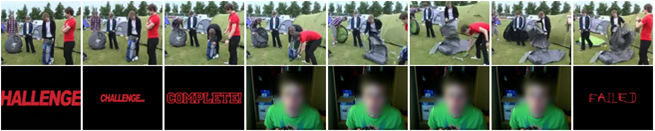
\includegraphics[width=1\textwidth]{teaser_image.png}
	\caption{Example video for "assembling a shelter" event in the TRECVID MED 2010 dataset. The top row shows the relevant frames while the bottom row shows the noisy frames.}
	\label{f_teaser}
\end{figure}

We are interested in the problem of video pooling for a more robust video representation. We consider a video as a layered structure where the lowest layer are frames, the top layer is the entire video, and the middle layers are the sequences of consecutive frames or the concatenation of lower layers. Based on this layered structure of video, we propose to use the sum-max video pooling to deal with noisy information in complex videos. Basically, we apply sum pooling at the low layer representation while using max pooling at the high layer representation. Sum pooling is used to keep sufficient relevant features at the low layer, while max pooling is used to retrieve the most relevant features at the high layer, therefore it can discard irrelevant features in the final video representation. \index{video representation}

Our work is most related to \cite{DBLP:journals/vlsisp/PhanNLTLDS14}, in which they proposed a segment-based approach to generate segment level representation using the sum pooling technique. Here we focus on different pooling techniques to generate the video representation. Experimental results on the TRECVID Multimedia Event Detection 2010 dataset shows the effectiveness of our method.

The rest of this chapter is organized as follows. Section 2 introduces the layered structure of video. Section 3 presents our sum-max pooling technique based on this layered structure. The experimental setup and experimental results are described in Section 4. Finally, Section 5 concludes this chapter with discussions on our future work.

\section{Layered Structure of Video} \index{layer structure}
\label{sec:format}
As mentioned in the previous section, pooling over the whole video is not effective for complex video representation because these videos can contain irrelevant information. The direct solution to remove these irrelevant information from the final video representation is to pool over the relevant parts only. However, it is also non-trivial to determine which parts of the video are relevant or not. 
\begin{figure}[!htb]
	\centering
	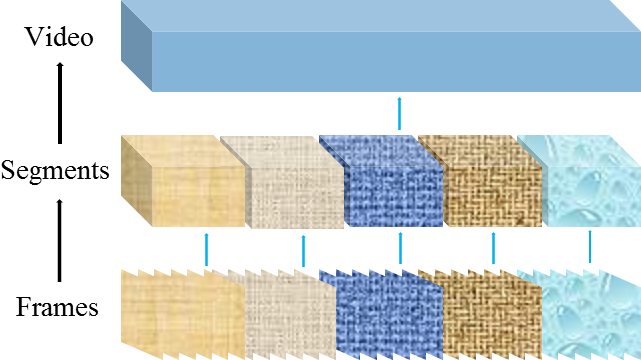
\includegraphics[width=1\textwidth]{layered.png}
	\caption{Illustration of layered structure of video.}
	\label{f_layer}
\end{figure}

The layered structure of video is a simply way to lessen the impact of irrelevant information. We define this layered structure as follows. The lowest layer are the frames of that video. The top layer is the entire video. The middle layers are the sequences of consecutive frames or the concatenation of lower layers. Figure \ref{f_layer} illustrates the layered structure in videos.

For the sake of simplicity, we only use one middle layer and the frame sequences in the middle layer are referred as segments in the rest of this chapter. In implementation, we choose the length of the segments varies in the following range: 15, 30, 45, 60, 75, 90, 105, 120, 135, 150, 165, 180, 195 and 210 seconds. We report the best segment length in Section \ref{c4_experiment}.

\section{Sum-max Video Pooling} \index{sum-max video pooling}
\label{sec:summax}
\begin{figure}
	\centering
	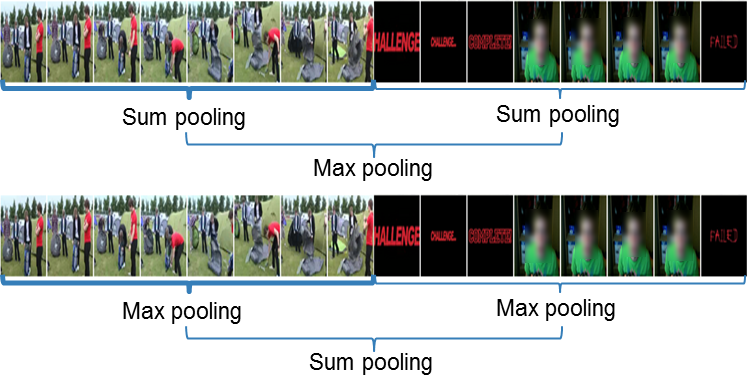
\includegraphics[width=1\textwidth]{summax_maxsum.png}
	\caption{Example of applying sum-max video pooling (top) and max-sum video pooling (bottom) methods on an ``assembling a shelter'' event video. It can be seen from the top image that after applying max pooling at the segment level, only relevant frames are encoded in the final representation.}
	\label{f_sum_max3}
\end{figure}

\begin{figure}
	\centering
	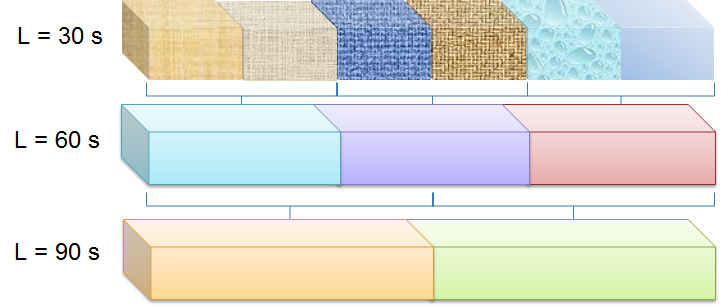
\includegraphics[width=1\textwidth]{efficient.png}
	\caption{Features from higher layers can be obtained from lower layers efficiently.}
	\label{f_efficient}
\end{figure}

\begin{figure}[!htb]
	\centering
	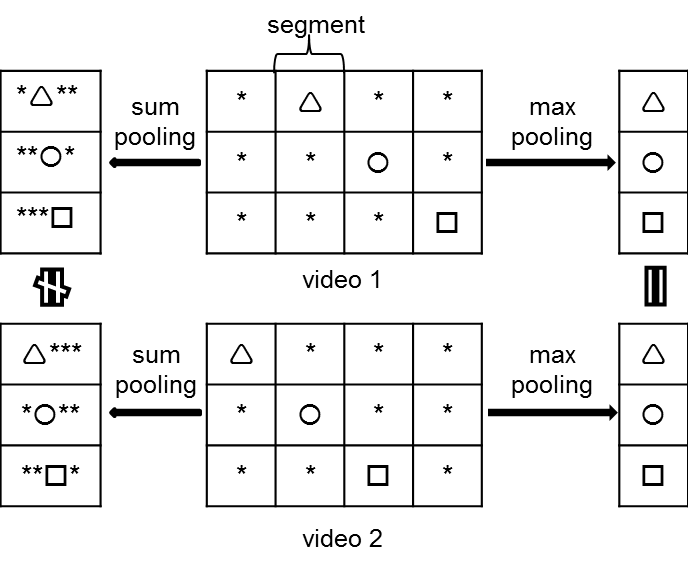
\includegraphics[width=1\textwidth]{sum_max.png}
	\caption{Illustration of sum-max video pooling. $\triangle$, O, $\Box$ represent relevant information; * represents different kinds of irrelevant information, which is popular in complex event data. Due to the native of the data, relevant information can appear in any part of the video, and can follow some temporal order. }
	\label{f_sum_max}
\end{figure}
\begin{figure*}[!htb]
	\centering
	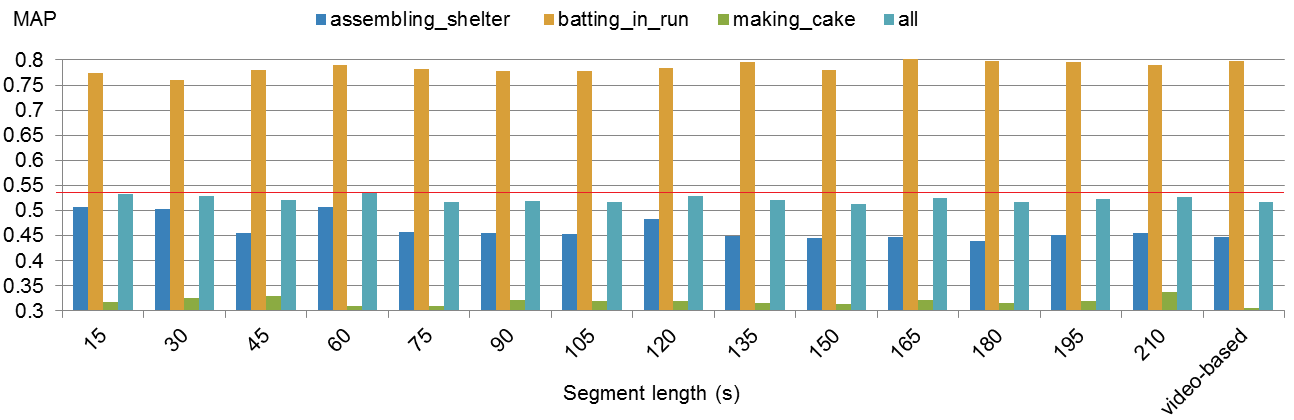
\includegraphics[width=1\textwidth]{sum_max_chart.png}
	\caption{Results on the MED 2010 dataset using the sum-max pooling technique at different segment lengths.}
	\label{f_sum_max_chart}
\end{figure*}
\begin{figure*}[!htb]
	\centering
	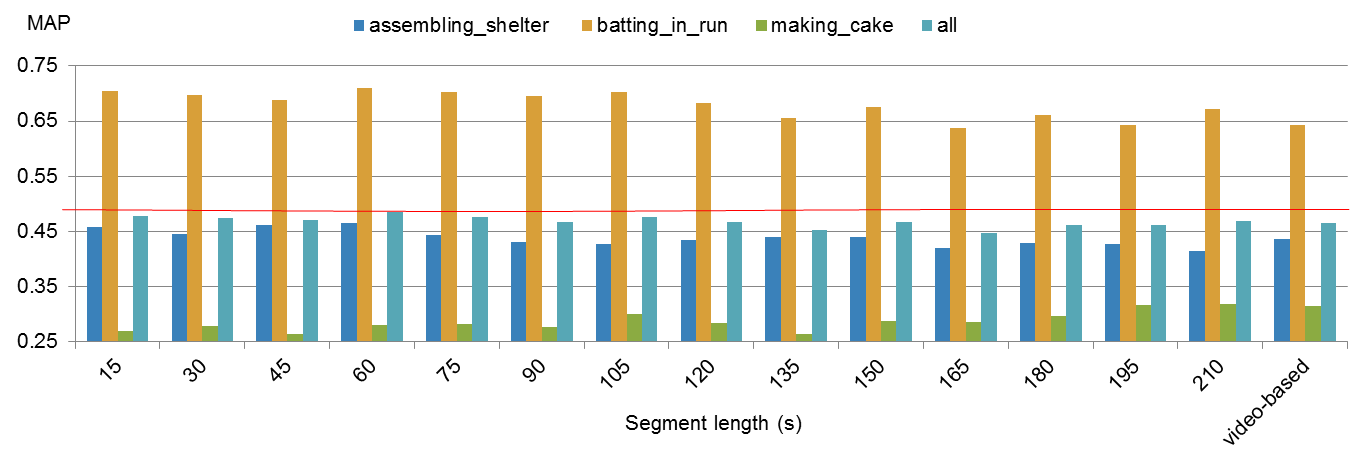
\includegraphics[width=1\textwidth]{max_sum_chart.png}
	\caption{Results on the MED 2010 dataset using the max-sum pooling technique at different segment lengths.}
	\label{f_max_sum_chart}
\end{figure*}
Our sum-max video pooling method is proposed based on the layered structure of video and consists of two steps: (1) Applying sum pooling to aggregate features from all frames of each segment to generate the feature representation of that segment; (2) Applying max pooling to aggregate the segment-level features to form the video representation. The max-sum video pooling can be obtained in the same way but different in that max pooling is applied first, then the sum pooling. It is worth noted that, sum video pooling and max video pooling are two special cases when we applying sum-max video pooling and max-sum video pooling for the whole video respectively. Examples of sum-max and max-sum video pooling are shown in Fig \ref{f_sum_max3}. 

In the context of bag-of-words model, suppose that there are N local descriptors in the video, each descriptor is denoted at $x_{n} \in R^{D}$, where n = 1,...,N and D is the feature dimension. Denote each visual word $m_{k} \in R^{D}$, where k = 1,...,K with K is number of visual words. $M = \{m_{k}\}$ is the set of visual words. The mid level coding of each descriptor can be expressed as $\phi_{n} = [\Phi_{1n},...,\Phi_{Kn}]$. Further suppose that the video contains \textit{S} segments. Denote $N_{s}$ is the number of local descriptors in segment \textit{s}. The sum-max and max-sum video pooling at each visual word can be defined as follows:
\begin{equation}\psi_{k} = Max_{s \in S}(\sum_{n \in N_{s}}\Phi_{kn})\end{equation}

\begin{equation}\psi_{k} = \sum_{s \in S}(Max_{n \in N_{s}}\Phi_{kn})\end{equation}

An intuitive example of sum-max pooling is shown in Fig \ref{f_sum_max}. As we can see, max pooling reserves the relevant information because noisy data tend to be varied, and none of any kind of them is dominant. In the contrast, sum pooling incorporates both relevant and irrelevant ones. Therefore, it is less representative than max pooling.

It is also worth noted that features from higher layers can be obtained from lower layers efficiently. In fact, we only need to extract feature one time. An illustration of features calculated from different segment lengths can be seen on Fig. \ref{f_efficient}.

\section{Experiment}
\label{c4_experiment}
\subsection{Experimental Setup}
We tested our method on TRECVID MED 2010 dataset. An event kit is provided with the definitions and textual descriptions for all the events for each dataset. The first dataset contains 3,468 videos, including 1,744 videos for training and 1,724 video clips for testing, containing a total of more than 110 video hours. In TRECVID MED 2010, there are 3 event classes: \textit{assembling a shelter} (E001), \textit{batting in a run} (E002), and \textit{making a cake} (E003).

We adopt the popular bag-of-words model to build our event recognition framework. At first, we use dense trajectory motion feature published by Wang \cite{wang:2011:inria-00583818:1} to calculate raw motion features as local trajectory descriptors. The library to extract these features is published online by the author\footnote{http://lear.inrialpes.fr/people/wang/dense\_trajectories}. The source code is customized for pipeline processing using only Motion Boundary Histogram (MBH) descriptor to save computing time but other parameters are set to default. 

In the coding step, we randomly select 1,000,000 dense trajectories for clustering to form a codebook of 4000 visual codewords. After that, the frequency histogram of the visual words is computed over each segment to generate the feature vector for that segment. Finally, we apply the sum-max pooling technique as described in Section \ref{sec:summax} to obtain the final video representation. We also adopt the soft assignment weighting scheme \cite{Jiang:2007:TOB} with 5 nearest neighbors to improve the performance of the ``bag-of-words'' approach.

In the learning and testing step, we use the popular Support Vector Machine (SVM) for event classification. In particular, we use the LibSVM library available online\footnote{http://www.csie.ntu.edu.tw/{\textasciitilde}cjlin/libsvm/} and adopt the one-vs.-rest scheme for multi-class classification. 

\subsection{Experimental Result and Analysis}

\subsubsection{On the MED 2010 dataset}
We report the results in terms of the Mean Average Precision (MAP). Results of sum-max video pooling and max-sum video pooling are showed in Fig \ref{f_sum_max_chart} and Fig \ref{f_max_sum_chart} respectively. Sum-max pooling improves the overall performance, especially for ``assembling a shelter'' event. The best performance is obtained at the segment length of 60 s (same as observed in \cite{DBLP:journals/vlsisp/PhanNLTLDS14}). Max-sum video pooling did not achieve good results compared to sum-max video pooling. The reason for the low performance of max-sum pooling can be due to the lost of relevant information when max-pooling is applied first. 

We also observed that the performance largely depends on the segment length and the event itself. For example, we can get better performance with short segment lengths for the event ``assembling a shelter'', while the event ``making a cake'' tends to have better performance with longer segments. 

We summarize our experimental results in Table \ref{t_med10}. The best performing feature is highlighted in bold for each event. In general, pooling over segments is more effective, i.e, sum-max pooling outperforms sum pooling and max-sum pooling outperforms max pooling. In the best case, sum-max video pooling outperforms the traditional sum pooling up to 2\% in terms of MAP.

\begin{table}
	\renewcommand{\arraystretch}{1.3}
	\caption{Performance comparison of different video pooling strategies on the MED 2010 dataset.}
	\label{t_med10}
	\centering
	\begin{tabular}{|c|c|c|c|c|}
		\toprule
		Event/MAP & \begin{tabular}[x]{@{}c@{}}Max\\pooling \end{tabular} & \begin{tabular}[x]{@{}c@{}}Sum\\pooling \end{tabular} & \begin{tabular}[x]{@{}c@{}}Max-sum\\pooling\\(at 60 s)\end{tabular} & \begin{tabular}[x]{@{}c@{}}Sum-max\\pooling\\(at 60 s)\end{tabular} \\
		%\bfseries \begin{tabular}[c]{@{}c@{}} CU\\(SIFT)\end{tabular}&
		%\bfseries \begin{tabular}[c]{@{}c@{}}CU (STIP,\\SIFT,\\MFCC)\end{tabular}\\
		\midrule
		E001&0.4365&0.4468&0.4646&\textbf{0.5072}
		\\
		\midrule
		E002&0.6434&\textbf{0.7988}&0.7103&0.7900
		\\
		\midrule
		E003&\textbf{0.3144}&0.3053&0.2806&0.3100
		\\
		\midrule
		All&0.4648&0.5170&0.4852&\textbf{0.5357}
		%&0.512&0.633
		\\
		\bottomrule
	\end{tabular}
\end{table}

\subsubsection{On the MED 2011 dataset}

In this experiment, we calculate the sum-max video pooling at different segment lengths including 8 s, 16 s, 32 s, 64 s, 128 s and 256 s. Results of our proposed methods on MED 2011 dataset are shown on Fig. \ref{f_med11_summax_kernel} and Fig. \ref{f_med11_summax_linear} respectively. Our best results are obtained at 8 s when using ${\chi}^2$ SVM and 32 s when using linear SVM.

\begin{figure*}[!htb]
	\centering
	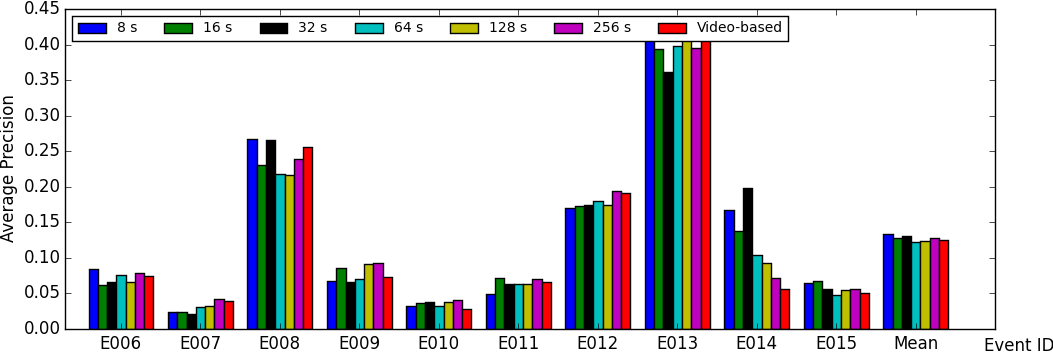
\includegraphics[width=1\textwidth]{med11_summax_kernel.png}
	\caption{Results on the MED 2011 dataset using the sum-max pooling technique at different segment lengths (${\chi}^2$ SVM).}
	\label{f_med11_summax_kernel}
\end{figure*}

\begin{figure*}[!htb]
	\centering
	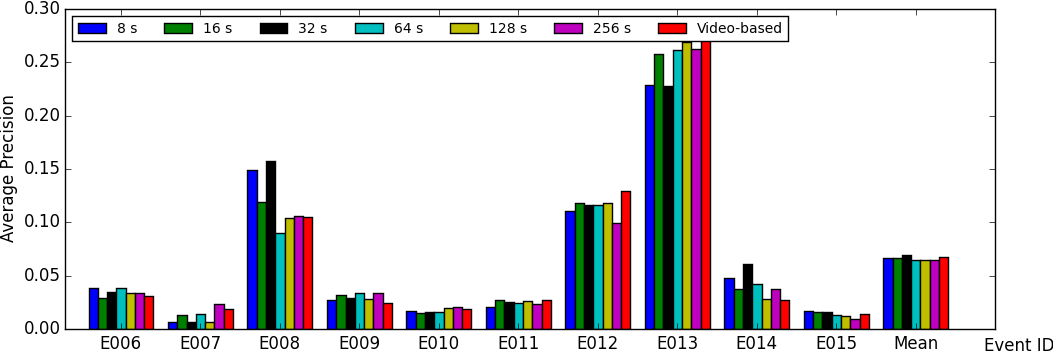
\includegraphics[width=1\textwidth]{med11_summax_linear.png}
	\caption{Results on the MED 2011 dataset using the sum-max pooling technique at different segment lengths (linear SVM).}
	\label{f_med11_summax_linear}
\end{figure*}


\section{Conclusion}
\label{sec:majhead}

We proposed to use a sum-max video pooling technique to combine both sum pooling and max pooling into a holistic video representation. This pooling technique is based on the layered structure of video. Preliminary results showed that this is an promising direction for video representation.

One limitation of the current approach is that the performance depends on the segment length. Therefore, we suggest to investigate a better approach to utilize the layered structure of video for video representation.

For video representation, temporal information is also very important. However, it is difficult to encode temporal information because video lengths are very varied. Therefore, exploring temporal pooling for video representation is also a good research direction.  


\chapter{Multimedia Event Detection Using Event-Driven Multiple Instance Learning}
\label{chapter5}
%\setlength{\epigraphrule}{0pt}
\epigraph{\textit{You never change things by fighting the existing reality.
		To change something, build a new model that makes the existing model obsolete.}}{ -- Buckminster Fuller}

% **************************** Define Graphics Path **************************
\ifpdf
    \graphicspath{{Chapter5/Figs/Raster/}{Chapter5/Figs/PDF/}{Chapter5/Figs/}}
\else
    \graphicspath{{Chapter5/Figs/Vector/}{Chapter5/Figs/}}
\fi


\section{Introduction}
The problem of recognizing complex event in videos has become a popular research topic due to the explosive growth of video data. A complex event can involve several actions or activities and happens in some particular settings. Therefore, recognizing complex event is more challenging than single action recognition. However, most complex detection systems are still based on the techniques that was developed for action recognition \cite{oneata2013action,Wang2013}. These methods basically extract and aggregate local feature descriptors from the whole video to create a unique video representation. This strategy might be not effective for complex event detection because it treats different parts of the video equally. Therefore, it neutralizes the important local information of an event.

\begin{figure}
	\centering
	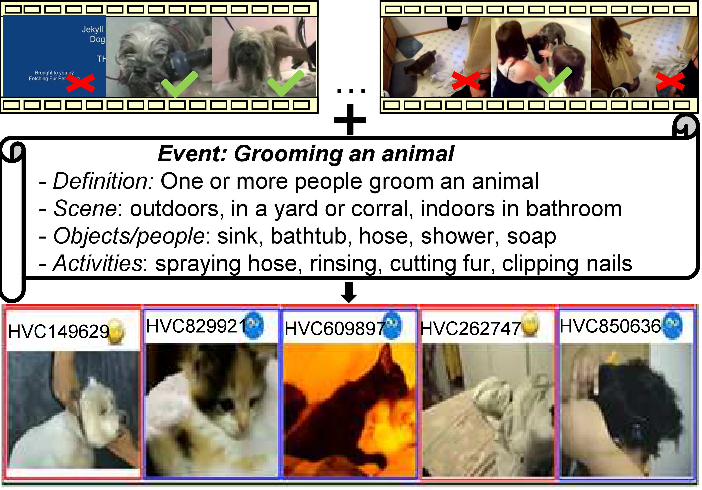
\includegraphics[width=1\textwidth]{figure_1.pdf}
	\caption{Event "Grooming an animal" in the TRECVID MED 2012 dataset. The event kit includes example videos and an event description which provides valuable cues to detect that event.}
	\label{figure_1}
\end{figure}

In practice, human can recognize a complex event by spotting several evidences in video \cite{bhattacharya2014minimally}. This paper also demonstrated that better performance can be obtained by leveraging positive and negative visual cues selected by humans. Therefore, it is important to automatically detect key evidences for event detection. Several researchers have been working on this direction. Tang \textit{et al.} \cite{tang2012learning} split the video into segments and models key segments and its duration as latent variables. Vahdat \textit{et al.} \cite{vahdat2013compositional} focus on intra-class variation by localizing only the most salient evidence using latent SVM. 
Lai \textit{et al.} \cite{lai2014video} detect salient instances in video based on a variant multiple instance learning. In another work \cite{lai2014recognizing}, they represent static and dynamic instances as sparse features and adopt a learning-to-rank strategy to detect key evidence. In general, these approaches are based on the assumption that segment annotation can be obtained from its video label. However, this is a weak assumption because the importance of each segment is not taken into account. 

On the other hand, the importance of a segment to an event can be obtained by matching its concept-based representation against the evidential description of that event. Some works have been using the event description for zero-shot event detection such as in \cite{chen2014event,wu2014zero}. To the best of our knowledge, no work has taken into account this information for detecting key evidence in videos. However, the evidential description of an event provides valuable information to detect that event. Example of an event description (excerpted) is shown in Fig. \ref{figure_1}. 

Motivated by this observation, we propose a new method, Event-driven Multiple Instance Learning (EDMIL), to learn key evidences for complex event detection. We treat each segment as an instance and model it in a multiple instance learning framework \cite{andrews2002support}, where each video is a "bag". The instance-event similarity is quantized into different levels of relatedness. Intuitively, the most (ir)relevant instances should have higher (dis)similarities. Therefore, we propose to learn the instance labels by jointly optimize the instance classifier and its related level. We evaluate our proposed method on the large scale TRECVID MED 2012 dataset. Comparing to other instance-based learning methods such as \cite{andrews2002support,lai2014video}, our method achieves a superior performance.

The remaining of this paper is organized as follows. In the next section, we present the method to calculate the instance-event similarity. Our proposed solution is introduced in Section \ref{method}. The experiments and results are shown in Section \ref{experiment}. Finally, Section \ref{conclusion} concludes the paper.

\section{Instance-Event Similarity}
In order to calculate the similarity between an instance and an event, we adopt a concept expansion strategy as in \cite{chen2014event}. Our method is similar in spirit, however, we apply at instance level which is more accurate. The outline of our method is illustrated in Fig. \ref{figure_2} and it consists of four steps.

\textbf{Step 1: Concept detection.} We use the concept collection that proposed in \cite{zhou2014places} to cover a wide range of concept that can appear in realistic videos. This collection contains C = 1183 categories including 205 scene categories from the Places Database and 978 object categories from the ImageNet 2012. The concept detection part is done by using the provided pre-trained model\footnote{http://places.csail.mit.edu}. To detect concept for the whole segment, we detect concept at sample frames and make the average aggregation.

\textbf{Step 2: Event representation.} We use standard natural language processing techniques to create the text-based event representation. At first, the event description is pre-processed by removing stop words and lemmatizing. It is then converted into a bag-of-words representation, where the dictionary is obtained from the English Wikipedia corpus. Tf-idf weighting scheme is also employed to put a higher weight on frequent as well as rare words.

\textbf{Step 3: Concept-event similarity.} To resolve the mismatch between words in the concept collection and event description, we adopt the concept expansion strategy \cite{chen2014event}. For each concept category, we add the 10 most similar concepts obtained from word2vec model\footnote{https://code.google.com/p/word2vec} to expand this category. It is then represented by a bag-of-words vector with tf-idf weights. Based on this representation, we can calculate the cosine similarity $s_{c}^{e}$ between each concept category and the event description. Table \ref{table1} shows top five most relevant concepts for some events on the MED 2012 dataset. 

\textbf{Step 4: Instance-event similarity.} Having obtained the concept score $x_{c}$ at each segment and the concept-event similarity as in Step 1 and Step 3, the instance-event similarity is calculated using the cosine similarity:
\begin{equation}
\label{eq1}
S_{i}^{e}=\frac{\sum_{c=1}^{C}s_{c}^{e}x_{c}}{\sqrt{\sum_{c=1}^{C}(s_{c}^{e})^{2}}\sqrt{\sum_{c=1}^{C}(x_{c})^{2}}},
\end{equation}
\begin{figure}
	\centering
	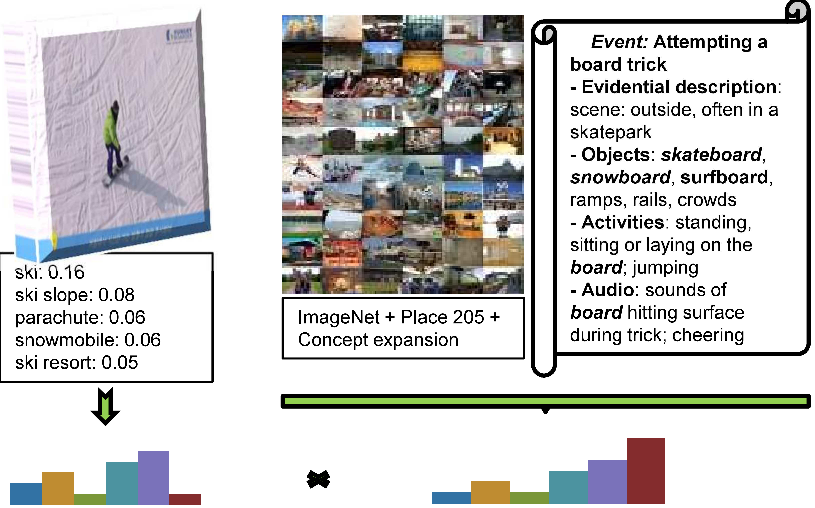
\includegraphics[width=1\textwidth]{figure_2.pdf}
	\caption{Outline of our method to calculate the instance-event similarity. Note that the concept expansion technique can bridge concept "ski" in the instance segment to the evidential description.}
	\label{figure_2}
\end{figure}


\begin{table}
		\centering
		\caption{Top five concepts discovered by our system for the first 10 events in the MED 2012 dataset.}
	\begin{tabular}{|c|l|}
		\hline
		\textbf{Event ID} & \multicolumn{1}{c|}{\textbf{Top five importance concepts discovered by our system}} \\ \hline
		E001              & Ski, slide rule, ski resort, ski mask, ice skating rink                             \\ \hline
		E002              & Meat loaf, white shark, food court, pop bottle, cleaver                             \\ \hline
		E003              & Anemone fish, pole, raft, sturgeon, boat deck                                       \\ \hline
		E004              & Groom, bridegroom, banquet hall, gown, altar                                        \\ \hline
		E005              & Jigsaw puzzle, bamboo forest, carpenter's kit, thatch, wooden spoon                 \\ \hline
		E006              & Table lamp, lampshade, torch, candle, custard apple                                 \\ \hline
		E007              & Recreational vehicle, car wheel, amphibian, scooter, sports car                     \\ \hline
		E008              & Monitor, chime, bell, whistle, ballroom                                             \\ \hline
		E009              & Recreational vehicle, amphibian, tank, car wheel, motor scooter                     \\ \hline
		E010              & Nail, bathtub, shower, fur coat, washbashin                                         \\ \hline
		E011              & Pizza, bagel, meat loaf, cheeseburger, vegetable garden                             \\ \hline
		E012              & Recreational vehicle, amphibian, tank, sports car, freight car                      \\ \hline
		E013              & Playground, volleyball, picnic area, sports car, table lamp                         \\ \hline
		E014              & Toaster, dish washer, washing machine, refrigerator, space heater                   \\ \hline
		E015              & Sewing machine, dragonfly, syringe, clothing store, construction site               \\ \hline
		E016              & Digital watch, classroom, CD player, crossword, stopwatch                           \\ \hline
		E017              & Tray, game room, cassette player, CD player, waiting room                           \\ \hline
		E018              & Backpack, walking stick, pop bottle, sleeping bag, plastic bag                      \\ \hline
		E019              & Tile roof, mortar, nail, jigsaw puzzle, drumstick                                   \\ \hline
		E020              & Ballpoint, pencil box, rubber eraser, quill pen, pencil sharpener                   \\ \hline
		E021              & Tricycle, mountain bike, scooter, bicycle-built-for-two, unicycle                   \\ \hline
		E022              & Toaster, refrigerator, dish washer, washing machine, space heater                   \\ \hline
		E023              & Schipperke, otter hound, bluestick, collie, Tibetan terrier                         \\ \hline
		E024              & Forest path, cellular telephone, phone booth, platform, dial phone                  \\ \hline
		E025              & Boxing ring, fairway, hand-held computer, bell cote, chime                          \\ \hline
	\end{tabular}
		\label{table1}
\end{table}

\section{Event-Driven Multiple Instance Learning}
\subsection{Problem Formalization} Suppose we have $V$ training videos, and $I_{v}$ instances in video $v$. We can calculate the similarity $S_{iv}^{e}$ between an instance $iv$ to a particular event $e$ using Eq. (\ref{eq1}). Suppose there is R level of relatedness from an instance to an event. We define two predict functions for positive and negative instances at level $r$ as follows.
\begin{equation}
\label{eq2}
P_{pos}(S_{iv}^{e},r) = 
\begin{cases}
1,& \text{if } Rank(S_{iv}^{e}) \leq r \\
-1,              & \text{otherwise}
\end{cases}\text{, and}
\end{equation}

\begin{equation}
\label{eq3}
P_{neg}(S_{iv}^{e},r) = 
\begin{cases}
-1,& \text{if } Rank(S_{iv}^{e}) \leq r \\
1,              & \text{otherwise}
\end{cases}\text{, }
\end{equation}
where $Rank(.)$ is the function to quantize a similarity into a related level. Note that smaller value of $r$ results a higher confidence in the predict functions. We now learn the parameters of the instance classifier jointly with the related level $r$ by optimizing the following objective function:
\label{method}
\begin{equation}
\label{eq4}
\begin{split}
\min_{\textbf{w},b,y,r} \frac{1}{2} \left \| \textbf{w} \right \|^{2} + C_{f} \sum_{v=1}^{V}\sum_{i=1}^{I_{v}}L_{f}\left ( y_{iv}, \textbf{w}^{T}\textbf{x}_{iv}+b \right ) \\
+ C_{p} \sum_{v=1}^{V}\sum_{i=1}^{I_{v}}L_{p}\left ( y_{iv}, P(S_{iv}^{e},r) \right ).
\end{split}
\end{equation}
$C_{f}$ and $C_{p}$ are cost parameters to control the influence of each loss function. Note that in the special case where $C_{p}=0$, the above formulation becomes a classic large-margin problem. $L_{f}(.)$ and $L_{p}(.)$ are two loss functions that will be jointly minimized. The first loss function minimizes the loss due to the classification mismatch based on the instance feature. The second one minimizes the loss due to the prediction obtained from the prior knowledge. Intuitively, when the related level $r$ increases, the first loss will also tend to increase while the second loss will become smaller, and vice versa. $L_{f}(.)$ and $L_{p}(.)$ can be any loss function. Throughout this paper, we use the standard hinge-loss function for $L_{f}(.)$:
$L_{f}\left ( y_{iv},\textbf{w}^{T}\textbf{x}_{iv}+b \right )=\text{max}(0,1-y_{iv}(\textbf{w}^{T}\textbf{x}_{iv}+b)),$
and the $L_{p}(.)$ function is defined so that it will penalize more on the high confident predictions:

$L_{p}\left ( y_{iv}, P(S_{iv}^{e},r) \right )= 
\begin{cases}
S_{iv}^{e},& \text{if } P(S_{iv}^{e},r) \neq y_{iv} \\
0,              & \text{otherwise}
\end{cases}.$

\subsection{Optimization Procedure}
The optimization problem in Eq. (\ref{eq4}) is a mixed-integer program which is not convex. In order to solve this problem, we apply the alternating optimization strategy to search for a suboptimal solution:
\begin{enumerate}
	\item{} Fix instance labels $y_{iv}$ and solve for \textbf{w} and \textit{b}. By fixing $y_{iv}$, the optimization problem becomes a classic SVM:
	
	$\min\limits_{\textbf{w},b}$ $\frac{1}{2} \left \| \textbf{w} \right \|^{2} + C_{f} \sum_{v=1}^{V}\sum_{i=1}^{I_{v}}L_{f}\left ( y_{iv}, \textbf{w}^{T}\textbf{x}_{iv}+b \right )$. 
	
	Thus it can be solved using a regular SVM solver.
	
	\item{} Fix \textbf{w} and \textit{b}, solve for $r$ and update $y_{iv}$. The problem now becomes: 
	
	$\min\limits_{y,r} C_{f} \sum_{v=1}^{V}\sum_{i=1}^{I_{v}}L_{f}\left ( y_{iv}, \textbf{w}^{T}\textbf{x}_{iv}+b \right ) 
	+ C_{p} \sum_{v=1}^{V}\sum_{i=1}^{I_{v}}L_{p}\left ( y_{iv}, P(S_{iv}^{e},r) \right ).$
	
	%\begin{equation}
	%\label{eq7}
	%\begin{split}
	%\min_{y,r} C_{f} \sum_{v=1}^{V}\sum_{i=1}^{I_{m}}L_{f}\left ( %y_{iv}, \textbf{w}^{T}\textbf{x}_{iv}+b \right ) \\
	%+ C_{p} \sum_{v=1}^{V}\sum_{i=1}^{I_{m}}L_{p}\left ( y_{iv}, %P(S_{iv}^{e},r) \right ).
	%\end{split}
	%\end{equation}
	We propose a greedy strategy to solve for this problem. At first, we iterate through all level of relatedness to search for the optimal $r$ by finding the minimum total loss when updating $y_{iv}$ using Eq. (\ref{eq2}, \ref{eq3}). Because the most positive and negative instances will be selected first, there will be a higher possibility to correct mismatched labels that were learned in the previous step. Lastly we update instance labels using Eq. (\ref{eq2}, \ref{eq3}) with the optimal $r$.
	
\end{enumerate}

Because this is not a convex optimization problem, the initialized values of $y_{iv}$ should be carefully selected. To this end, we use the same initilization method as in \cite{andrews2002support,lai2014video}, where instance labels are same with its "bag" (video) label. 

It is also worth noted that the optimization framework only keeps updating the instance labels while the instance features are unchanged. Thus it is a good practice to use the pre-computed kernel technique for optimizing \textbf{w} and \textit{b}. In fact, although our method is more complex, it only takes around 5 minutes for training one model, compared to 40 minutes that was reported in \cite{lai2014video}. 
\section{Experiments}
\subsection{Dataset} To evaluate our proposed method, we conducted experiments on the large scale TRECVID MED 2012 dataset\footnote{http://www.nist.gov/itl/iad/mig/med12.cfm}. This dataset provides the definition for 25 complex events. The first ten event names are listed in Table \ref{table1}. We follow the setting by \cite{lai2014video} to divide this video collection into training and testing parts. These parts contain 3,878 and 1,938 videos respectively.

\subsection{Experimental setup} At first, original videos are scaled down to 320 x 240 with keeping the aspect ratio. Key frames are sampled at every 2 seconds from the resized video. The segment length is set to 8 seconds as suggested in \cite{vahdat2013compositional}. To extract feature for each segment, we use the Improved Dense Trajectories feature proposed by Wang and Schmid \cite{Wang2013}. Motion Boundary Histogram (MBH) is used to represent extracted trajectories because it can handle camera motion, which is prevalent in realistic videos. For learning, we use our framework jointly with the linear SVM. The cost parameters $C_{f}$ and $C_{p}$ are selected by cross-validation in the range of $\{0.1, 1, 10, 100\}$. At the testing step, video-level score is obtained by averaging over all instance scores. Finally we use the standard evaluation metric on MED, Mean Average Precision (mAP), to report the performance.

\begin{figure}
	\centering
	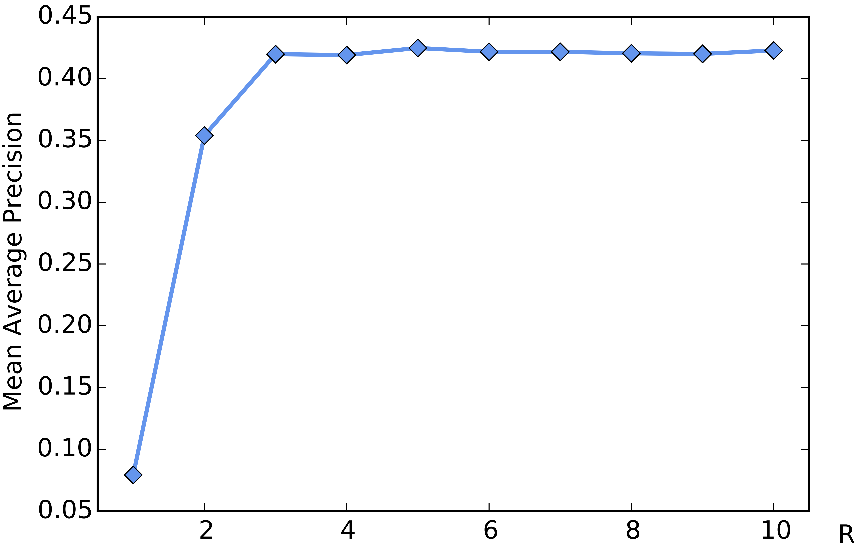
\includegraphics[width=1\textwidth]{figure_3.pdf}
	\caption{Optimal number of related levels.}
	\label{figure_3}
\end{figure}


\begin{figure*}
	\centering
	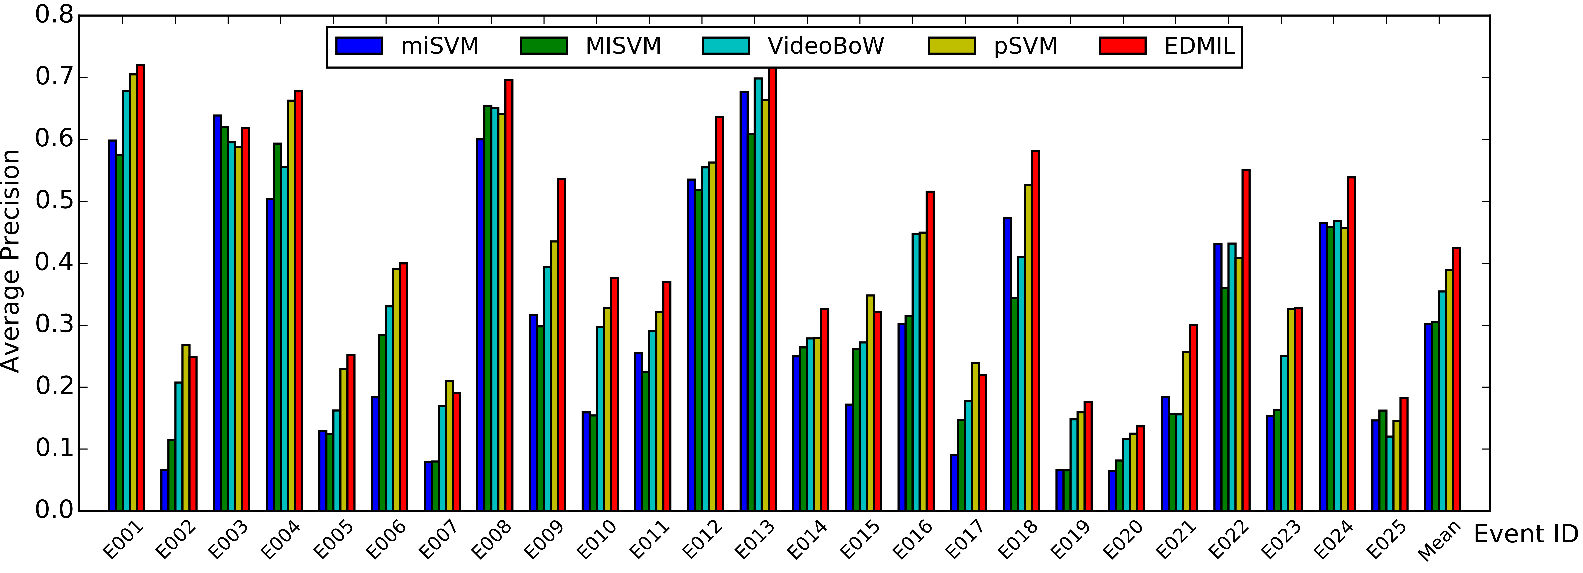
\includegraphics[width=1\textwidth]{figure_4.pdf}
	\caption{Evaluation results of 25 events in the TRECVID MED 2012 dataset. The mean APs are 0.3015 (miSVM), 0.3051 (MISVM), 0.3544 (VideoBOW), 0.3890 (pSVM) and 0.4246 (Ours).}
	\label{figure_4}
\end{figure*}

\subsection{Baseline methods} To compare our methods with following baselines: miSVM, MISVM \cite{andrews2002support}, VideoBOW and pSVM \cite{lai2014video}. At first, because our method is based on the Multiple Instance Learning (MIL) framework, we evaluate two MIL solutions: miSVM and MISVM that were proposed by the authors in \cite{andrews2002support}. The VideoBOW method is the standard approach where local features are aggregated from the whole video. We also compare our method with the recently proposed pSVM which was adopted in \cite{lai2014video} for TRECVID MED. For all the baseline methods, except VideoBOW, we utilize the codes provided by the authors to test with our features.


\subsection{Experimental results}
At first, we conduct experiments to find the optimal value of R. We select R in the range from 1 to 10. The overall performance is shown in Fig. \ref{figure_3}. We obtain the peak performance with R around 5. Small values of R tend to get low performances. This indicates that the prediction of prior knowledge is not always good, and learning jointly with instance features is necessary. The performance becomes saturated when R > 5. Therefore, we fix the value of R to 5 for further experiments.

The performance of each baseline method as well as our method (EDMIL) are shown in Fig. \ref{figure_4}. Our method significantly outperforms other baselines. For the best baseline, our method relatively outperforms by 10\%. Our instance-based classifier can also provide key evidences for event detection. Example of key evidences detected by our system can be seen in Fig. \ref{figure_5}. 
\label{experiment}

\begin{figure}
	\centering
	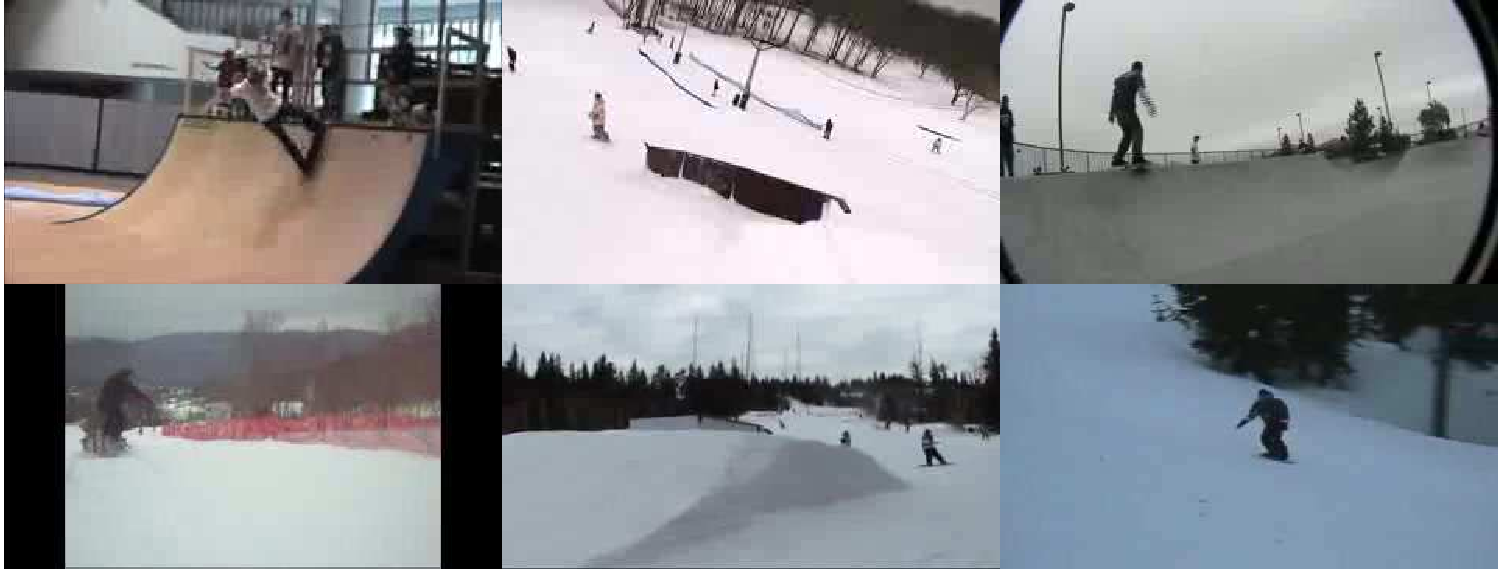
\includegraphics[width=1\textwidth]{figure_5.pdf}
	\caption{The top 6 key evidences detected by our system for the event "Attempting board trick". The dominance of ski-related instances is reasonable.}
	\label{figure_5}
\end{figure}

\section{Conclusions}
\label{conclusion}
We propose a new method to detect event in videos from its key evidences. Our method differs from others in that we utilize the evidential description provided for each event. Given this supportive information, we search for key evidences by jointly optimizing with instance feature in a variant of multiple instance learning framework. As a result, we obtained a superior event detection performance.


\chapter{Conclusion}
\label{chapter6}

%\setlength{\epigraphrule}{0pt}
\epigraph{\textit{If you can't fly then run, if you can't run then walk, if you can't walk then crawl, but whatever you do you have to keep moving forward.}}{ -- Martin Luther King Jr.}

% **************************** Define Graphics Path **************************
\ifpdf
    \graphicspath{{Chapter6/Figs/Raster/}{Chapter6/Figs/PDF/}{Chapter6/Figs/}}
\else
    \graphicspath{{Chapter6/Figs/Vector/}{Chapter6/Figs/}}
\fi

\section{Summary}

We made following contributions:

\begin{itemize}
	\item We propose using a segment-based approach to overcome the limitations of  the video-based approaches. The basic idea is to examine shorter segments instead of using the representative frames or entire video. We carry thorough experiments to verify our proposed method by investigating different strategies to decompose a video into segments. These strategies include uniform segment sampling and 
	
	\item We propose a new video pooling strategy, called sum-max video pooling, to deal with noisy information in complex videos. This pooling technique is based on the layer structure of video. Basically, we apply sum pooling at the low layer representation while using max pooling at the high layer representation. Sum pooling is used to keep sufficient relevant features at the low layer, while max pooling is used to retrieve the most relevant features at the high layer, therefore it can discard irrelevant features in the final video representation. 
	
	\item We propose a new method, named Event-driven Multiple Instance Learning (EDMIL), to learn key evidences for complex event detection. We treat each segment as an instance and model it in a multiple instance learning framework \cite{andrews2002support}, where each video is a "bag". The instance-event similarity is quantized into different levels of relatedness. Intuitively, the most (ir)relevant instances should have higher (dis)similarities. Therefore, we propose to learn the instance labels by jointly optimizing the instance classifier and its related level.	
	
\end{itemize}
	
\section{Future Work}



% ********************************** Back Matter *******************************
% Backmatter should be commented out, if you are using appendices after References
%\backmatter

% ********************************** Bibliography ******************************
%\begin{spacing}{0.9}

% To use the conventional natbib style referencing
% Bibliography style previews: http://nodonn.tipido.net/bibstyle.php
% Reference styles: http://sites.stat.psu.edu/~surajit/present/bib.htm

\bibliographystyle{apalike}
%\bibliographystyle{plainnat} % use this to have URLs listed in References
\cleardoublepage
\bibliography{References/references} % Path to your References.bib file


% If you would like to use BibLaTeX for your references, pass `custombib' as
% an option in the document class. The location of 'reference.bib' should be
% specified in the preamble.tex file in the custombib section.
% Comment out the lines related to natbib above and uncomment the following line.

%\printbibliography[heading=bibintoc, title={References}]

% ********************************** Appendices ********************************

\begin{appendices} % Using appendices environment for more functunality

% ******************************* Thesis Appendix A ****************************
\chapter{TRECVID MED 2013 Results} 

\ifpdf
\graphicspath{{Appendix1/Figs/Raster/}{Appendix1/Figs/PDF/}{Appendix1/Figs/}}
\else
\graphicspath{{Appendix1/Figs/Vector/}{Appendix1/Figs/}}
\fi

In this appendix, we briefly introduce our Multimedia Event Detection system for TRECVID MED 2013. We use both audio and visual features with Bag-of-Words and Fisher Vector Representation. Our MED framework consists of following steps: preprocessing, feature extraction, feature representation and event classification.

\section{Preprocessing} At first, all videos are normalized to around 320x240. We fix the width dimension to 320 and change the height so that the aspect ratios are kept. The audio channels are removed from resized videos to save disk space. After that, we extract one representative keyframe from resized videos at every 2 seconds and audio feature from the original videos. 

\section{Feature Extraction} We use feature from different modalities to model multimedia events: still image features, motion features and audio features. We use the standard SIFT with Hessian Laplace detector for extracting still image feature. For motion feature, we use Dense Trajectories with MBH descriptor. We use the MFCC for extracting audio feature. 

\section{Feature Representation} Bag-of-Words representation is a simple way to encode local features. It is the frequency histogram of local descriptors that are assigned to the nearest clusters. In the implementation, we randomly select 1,000,000 local descriptors to train the codebook with 4,000 codewords. The soft assignment technique is also employed to reduce the quantization errors. For Fisher vector, we use the codebook size of 256 clusters which are generated using the Gaussian Mixture Model (GMM). We further improve the expressiveness of Fisher vector by applying PCA for reducing feature dimension, i.e 80-d for SIFT and 128-d for MBH. 

\section{Event Classification}
We use the popular Support Vector Machine (SVM) for classification. All the positive videos are considered as positive samples and the remaining videos are considered as negative samples (including near miss videos). We use the chi-square kernel for training bag-of-words histogram features and linear kernel for training features encoded by Fisher vector.

\section{Result and Conclusion} We observed that Fisher vector representation is consistently better the traditional bag-of-words histogram representation. The motion features archived the highest performance in terms of single feature comparison, followed by image features and audio features. Furthermore, these features are highly complementary, so their combination achieved the best performance. We also observed a little performance gain when combining both Fisher vector and bag-of-words feature encoding. Based on these observations, we submitted the FullSys system based on the combination of audio or visual features. Our results (NII Team) on the 100Ex setting is shown in Fig. \ref{med2013_result}. Our rank is 4th out of 18 participants.

\begin{figure}
	\centering
	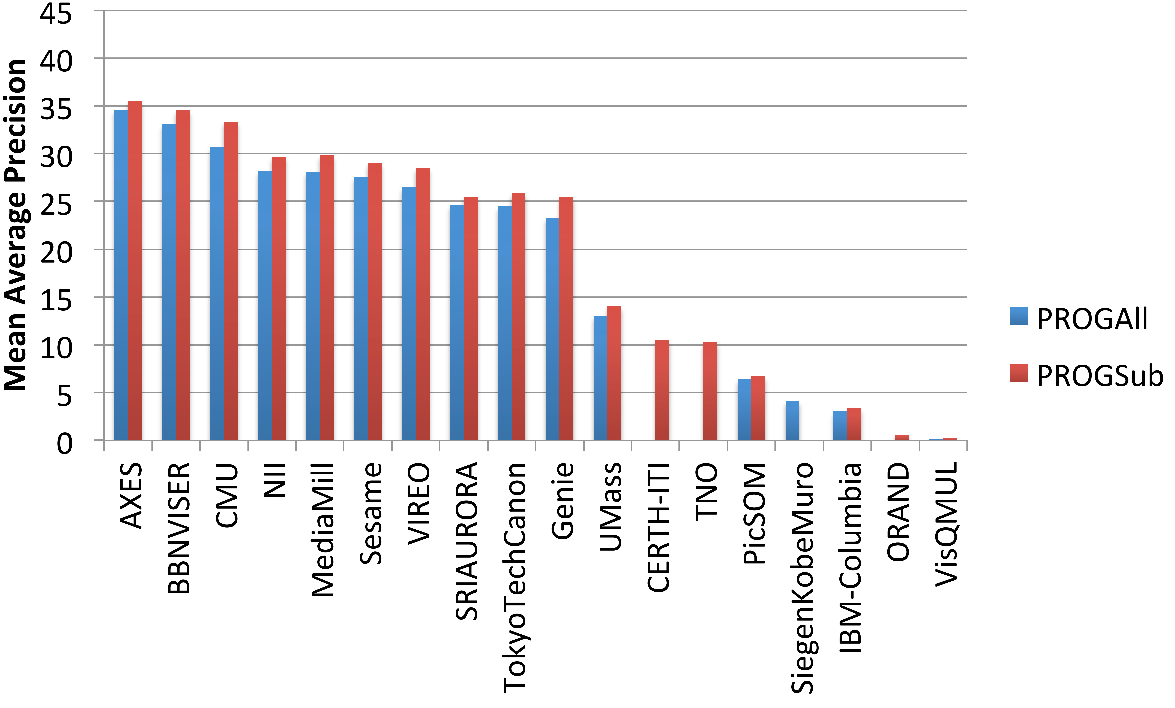
\includegraphics[width=1\textwidth]{results.pdf}
	\caption{Comparison of our MED 2013 system with others on the full evaluation set for the Pre-specified task. Results are sorted in the descending order of performance on the EK100 setting.}
	\label{med2013_result}
\end{figure} 
% ******************************* Thesis Appendix B ********************************

\chapter{TRECVID MED 2014 results}

\ifpdf
\graphicspath{{Appendix2/Figs/Raster/}{Appendix2/Figs/PDF/}{Appendix2/Figs/}}
\else
\graphicspath{{Appendix2/Figs/Vector/}{Appendix2/Figs/}}
\fi

In MED 2014, we study some technical improvements for motion feature and image features over our MED 2014 System.

\textbf{For Motion Features.} We use the improved version of Dense Trajectories motion feature \cite{Wang2013}. To describe trajectories, we choose to use both HOGHOF and MBH descriptors, which have been proved to be effective for MED by AXES team \cite{aly2013axes}. In order to combine these descriptors, we train two independent GMM codebooks. After that Fisher vector is used to encode feature from each descriptor independently. The resulting representation at video level of each descriptor is normalized by power normalization and L2 normalization. Finally these two feature vectors are concatenated to form the final representation of each video.

\textbf{For Image Features.} We apply two technical improvements on the image feature. At first, a new way of video level feature representation is used to pool feature from its keyframe-based representation. In MED 2013 system, we aggregated local descriptors from all sampled frames in video without explicitly calculating keyframe-based features. For this year's system, Fisher vector is encoded for each sampled frame and normalized using power and L2 normalization. Features from these sampled frames are averaged to form the video level representation. The second technical improvement is using RootSIFT features \cite{arandjelovic2012three}. We have applied RootSIFT with different implementation of SIFT features such as the one use in \cite{mikolajczyk2005performance}, VLFeat \cite{vedaldi08vlfeat}, and Color Descriptor \cite{vandeSandeTPAMI2010}. Finally we chose to use VLFeat because it achieved the best performance in our evaluation framework.

We evaluated the performance of new components on the KINDREDTEST 13 dataset. All results are reported in terms of Mean Average Precision (MAP). Performance comparison of motion features and image features are shown in Table \ref{t_motion} and Table \ref{t_sift} respectively. 

\begin{table}
	\renewcommand{\arraystretch}{1.3}	
	\caption{Performance comparison of different motion feature configurations.}
	\label{t_motion}
	\centering
	\begin{tabular}{cccll}
		\cline{1-3}
		\multicolumn{1}{|c|}{MED13 System}                                                       & \multicolumn{2}{c|}{MED14 System}                                                                                                                                                                            &  &  \\ \cline{1-3}
		\multicolumn{1}{|c|}{\begin{tabular}[c]{@{}c@{}}Dense Trajectories\\ (MBH)\end{tabular}} & \multicolumn{1}{c|}{\begin{tabular}[c]{@{}c@{}}Improved Dense \\ Trajectories (MBH)\end{tabular}} & \multicolumn{1}{c|}{\begin{tabular}[c]{@{}c@{}}Improved Dense \\ Trajectories (HOGHOF + MBH)\end{tabular}} &  &  \\ \cline{1-3}
		\multicolumn{1}{|c|}{28.33}                                                              & \multicolumn{1}{c|}{35.07}                                                                       & \multicolumn{1}{c|}{40.77}                                                                                &  &  \\ \cline{1-3}
		\multicolumn{1}{l}{}                                                                     & \multicolumn{1}{l}{}                                                                             & \multicolumn{1}{l}{}                                                                                      &  & 
	\end{tabular}
\end{table}
\begin{table}
	\renewcommand{\arraystretch}{1.3}
	\renewcommand{\arraystretch}{1.3}	
	\caption{Performance comparison of different image feature configurations.}
	\label{t_sift}
	\centering
	\begin{tabular}{cccll}
		\cline{1-3}
		\multicolumn{1}{|c|}{MED13 System} & \multicolumn{2}{c|}{MED14 System}                                                                                                                                                        &  &  \\ \cline{1-3}
		\multicolumn{1}{|c|}{SIFT}         & \multicolumn{1}{c|}{\begin{tabular}[c]{@{}c@{}}SIFT\\ (New aggregation)\end{tabular}} & \multicolumn{1}{c|}{\begin{tabular}[c]{@{}c@{}}SIFT\\ (New aggregation + RootSIFT)\end{tabular}} &  &  \\ \cline{1-3}
		\multicolumn{1}{|c|}{23.41}        & \multicolumn{1}{c|}{24.24}                                                            & \multicolumn{1}{c|}{27.02}                                                                       &  &  \\ \cline{1-3}
		\multicolumn{1}{l}{}               & \multicolumn{1}{l}{}                                                                  & \multicolumn{1}{l}{}                                                                             &  & 
	\end{tabular}
\end{table}

Unfortunately, we could not finish running the best configuration for motion features, so we use the same configuration as previous year because it took less time. For image feature, we used the improved version. We also used the late fusion technique to combine audio and visual features in our final submission. For related videos, we fixed our system to use them as negative training samples for both EK10 and EK100 settings. We participated in the full evaluation set containing around 200K videos for both Pre-specified (PS) and Adhoc (AH) tasks.

\textbf{Results and Conclusions.} Results of our MED system is shown in Fig. \ref{fig:results}. Our ranks was 11th out of 12 teams in the EK10 setting and 10th in the EK100 setting. This observation is same for both PS and AH tasks. Compared to top MED systems, our system is significantly worse in the EK10 setting. For example, our performance are 67\% and 41\% relatively to the best MED system in the EK100 and EK10 respectively. We have learnt that top performance system have incorporated semantic concept detection, which can be more helpful when number of training videos are limited. This might be the reason for the significant drop on the performance of our EK10 system.

\begin{figure}
	\centering
	\begin{subfigure}{\textwidth}
		\centering
		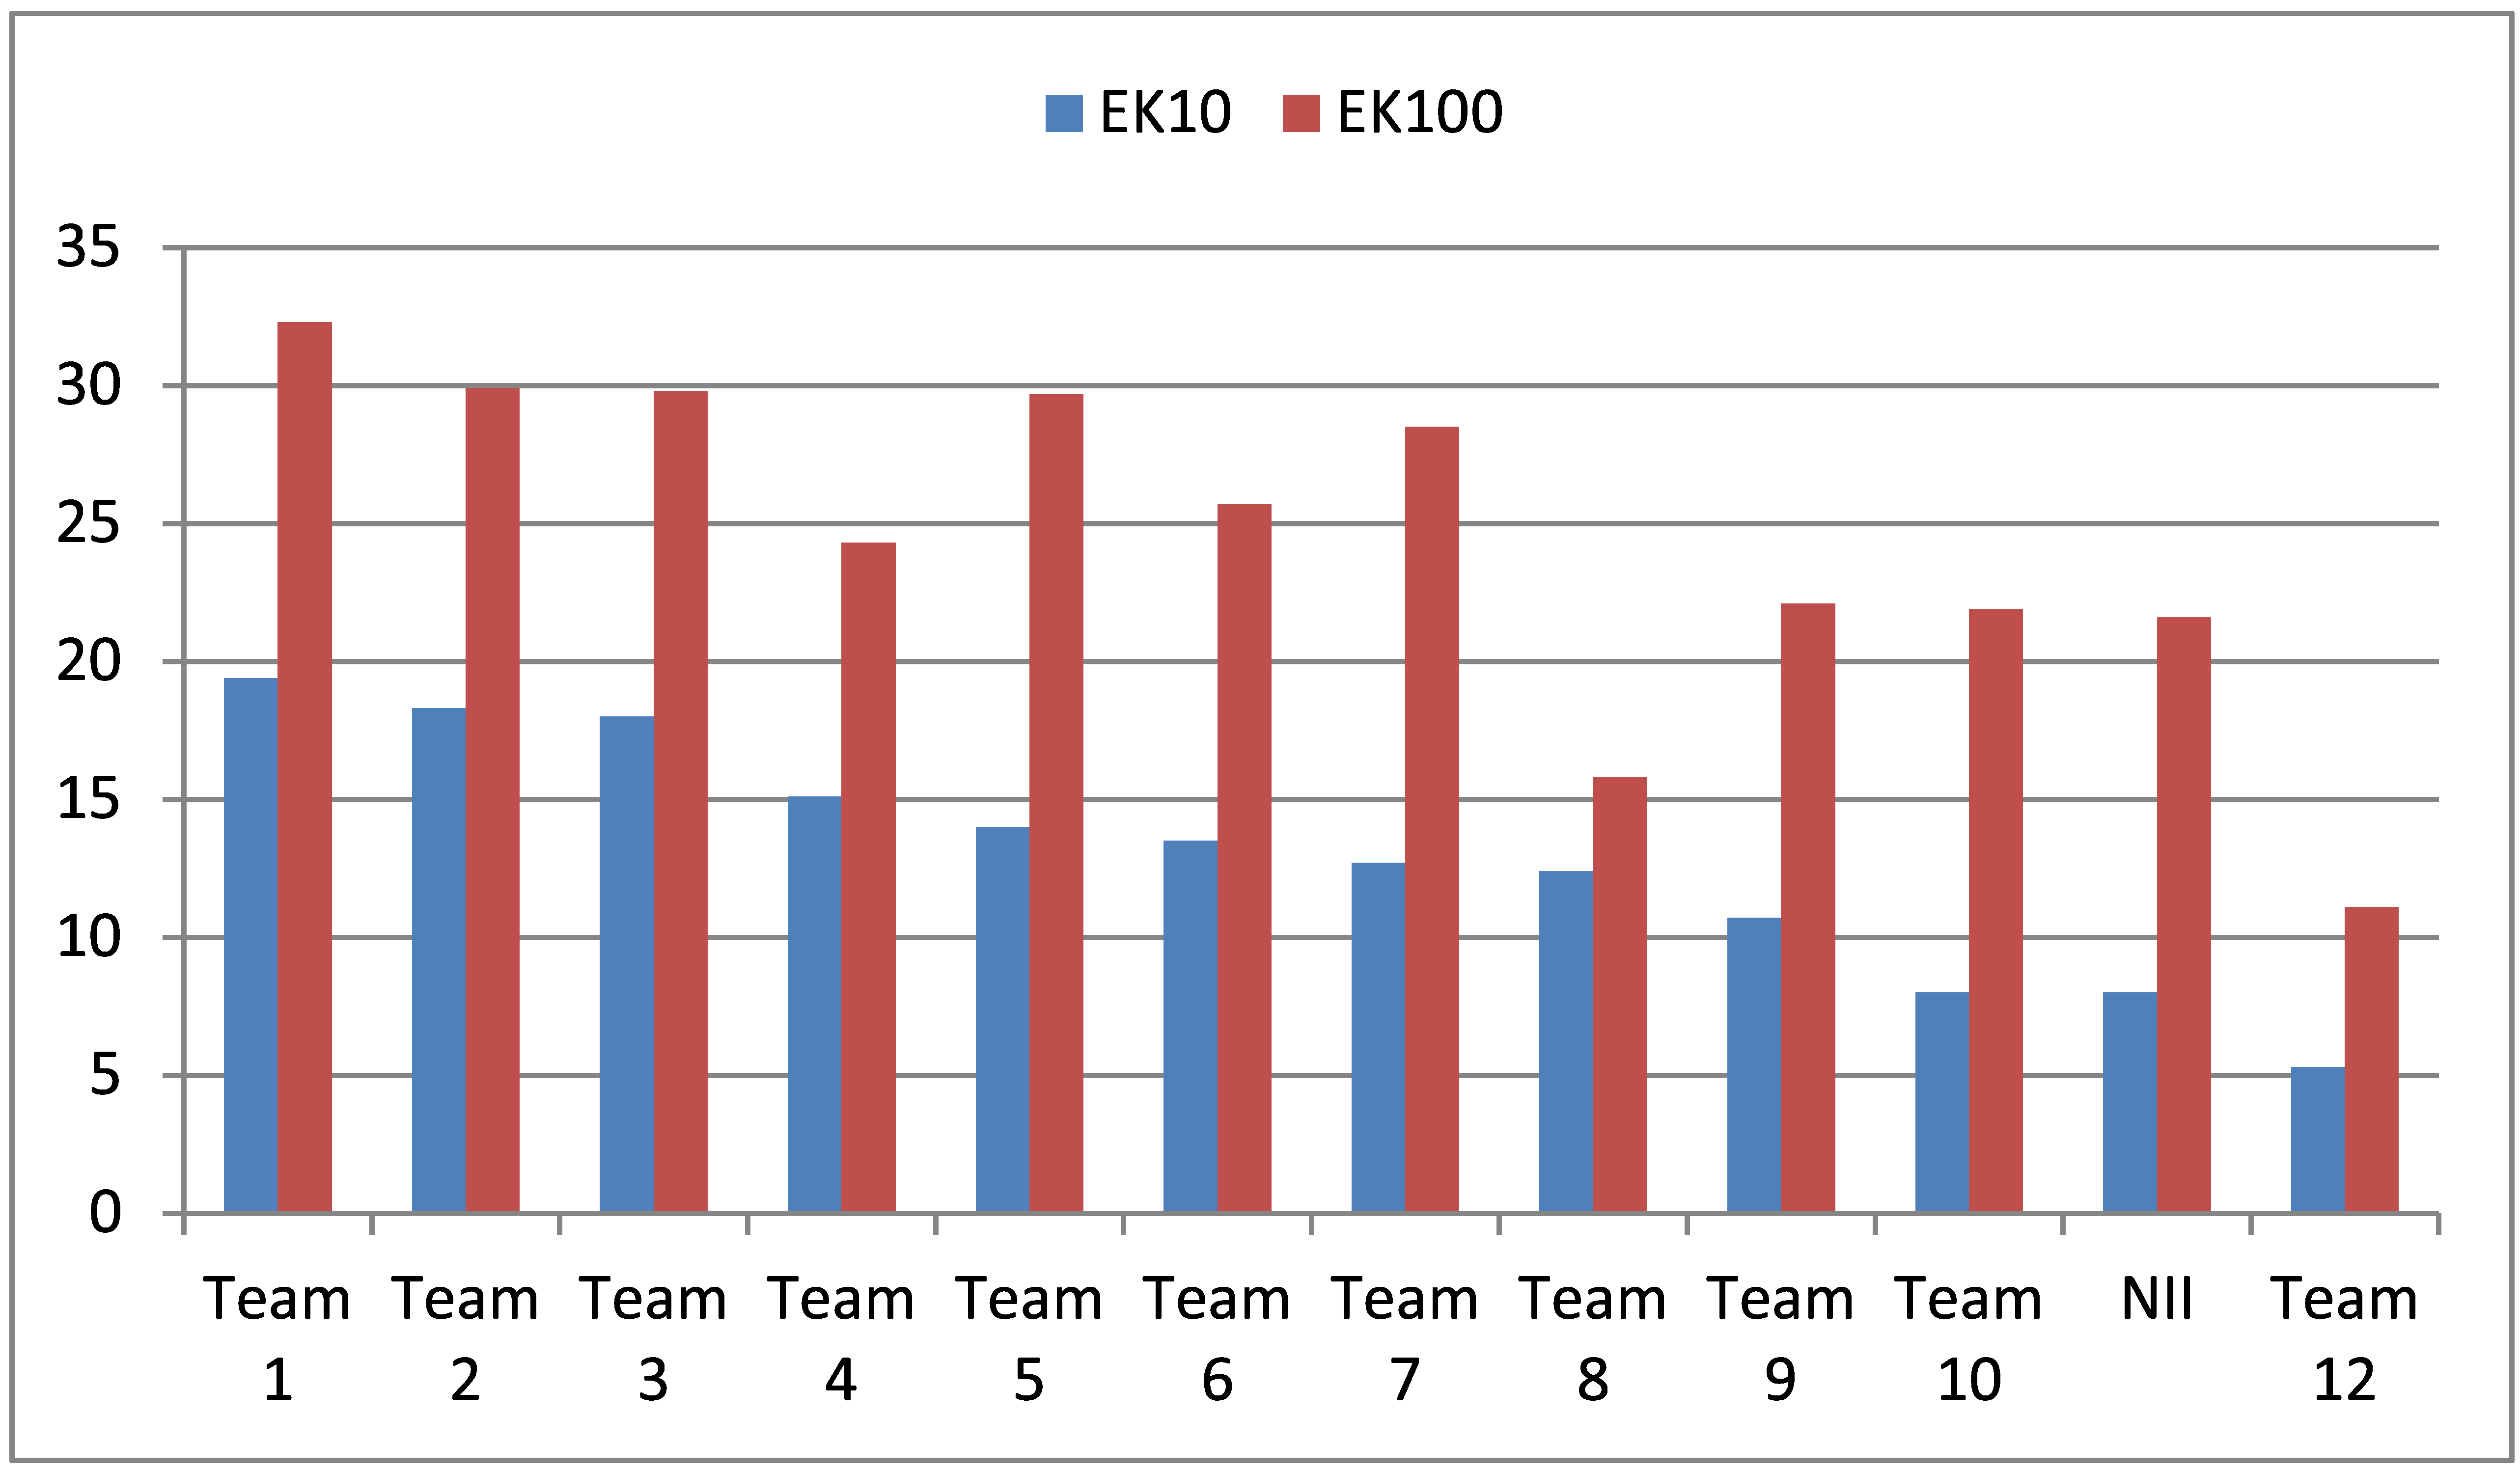
\includegraphics[width=1\linewidth]{med_result_ps.pdf}
		\caption{Pre-Specified systems}
		\label{fig_result_ps}
	\end{subfigure} 
	\begin{subfigure}{\textwidth}
		\centering
		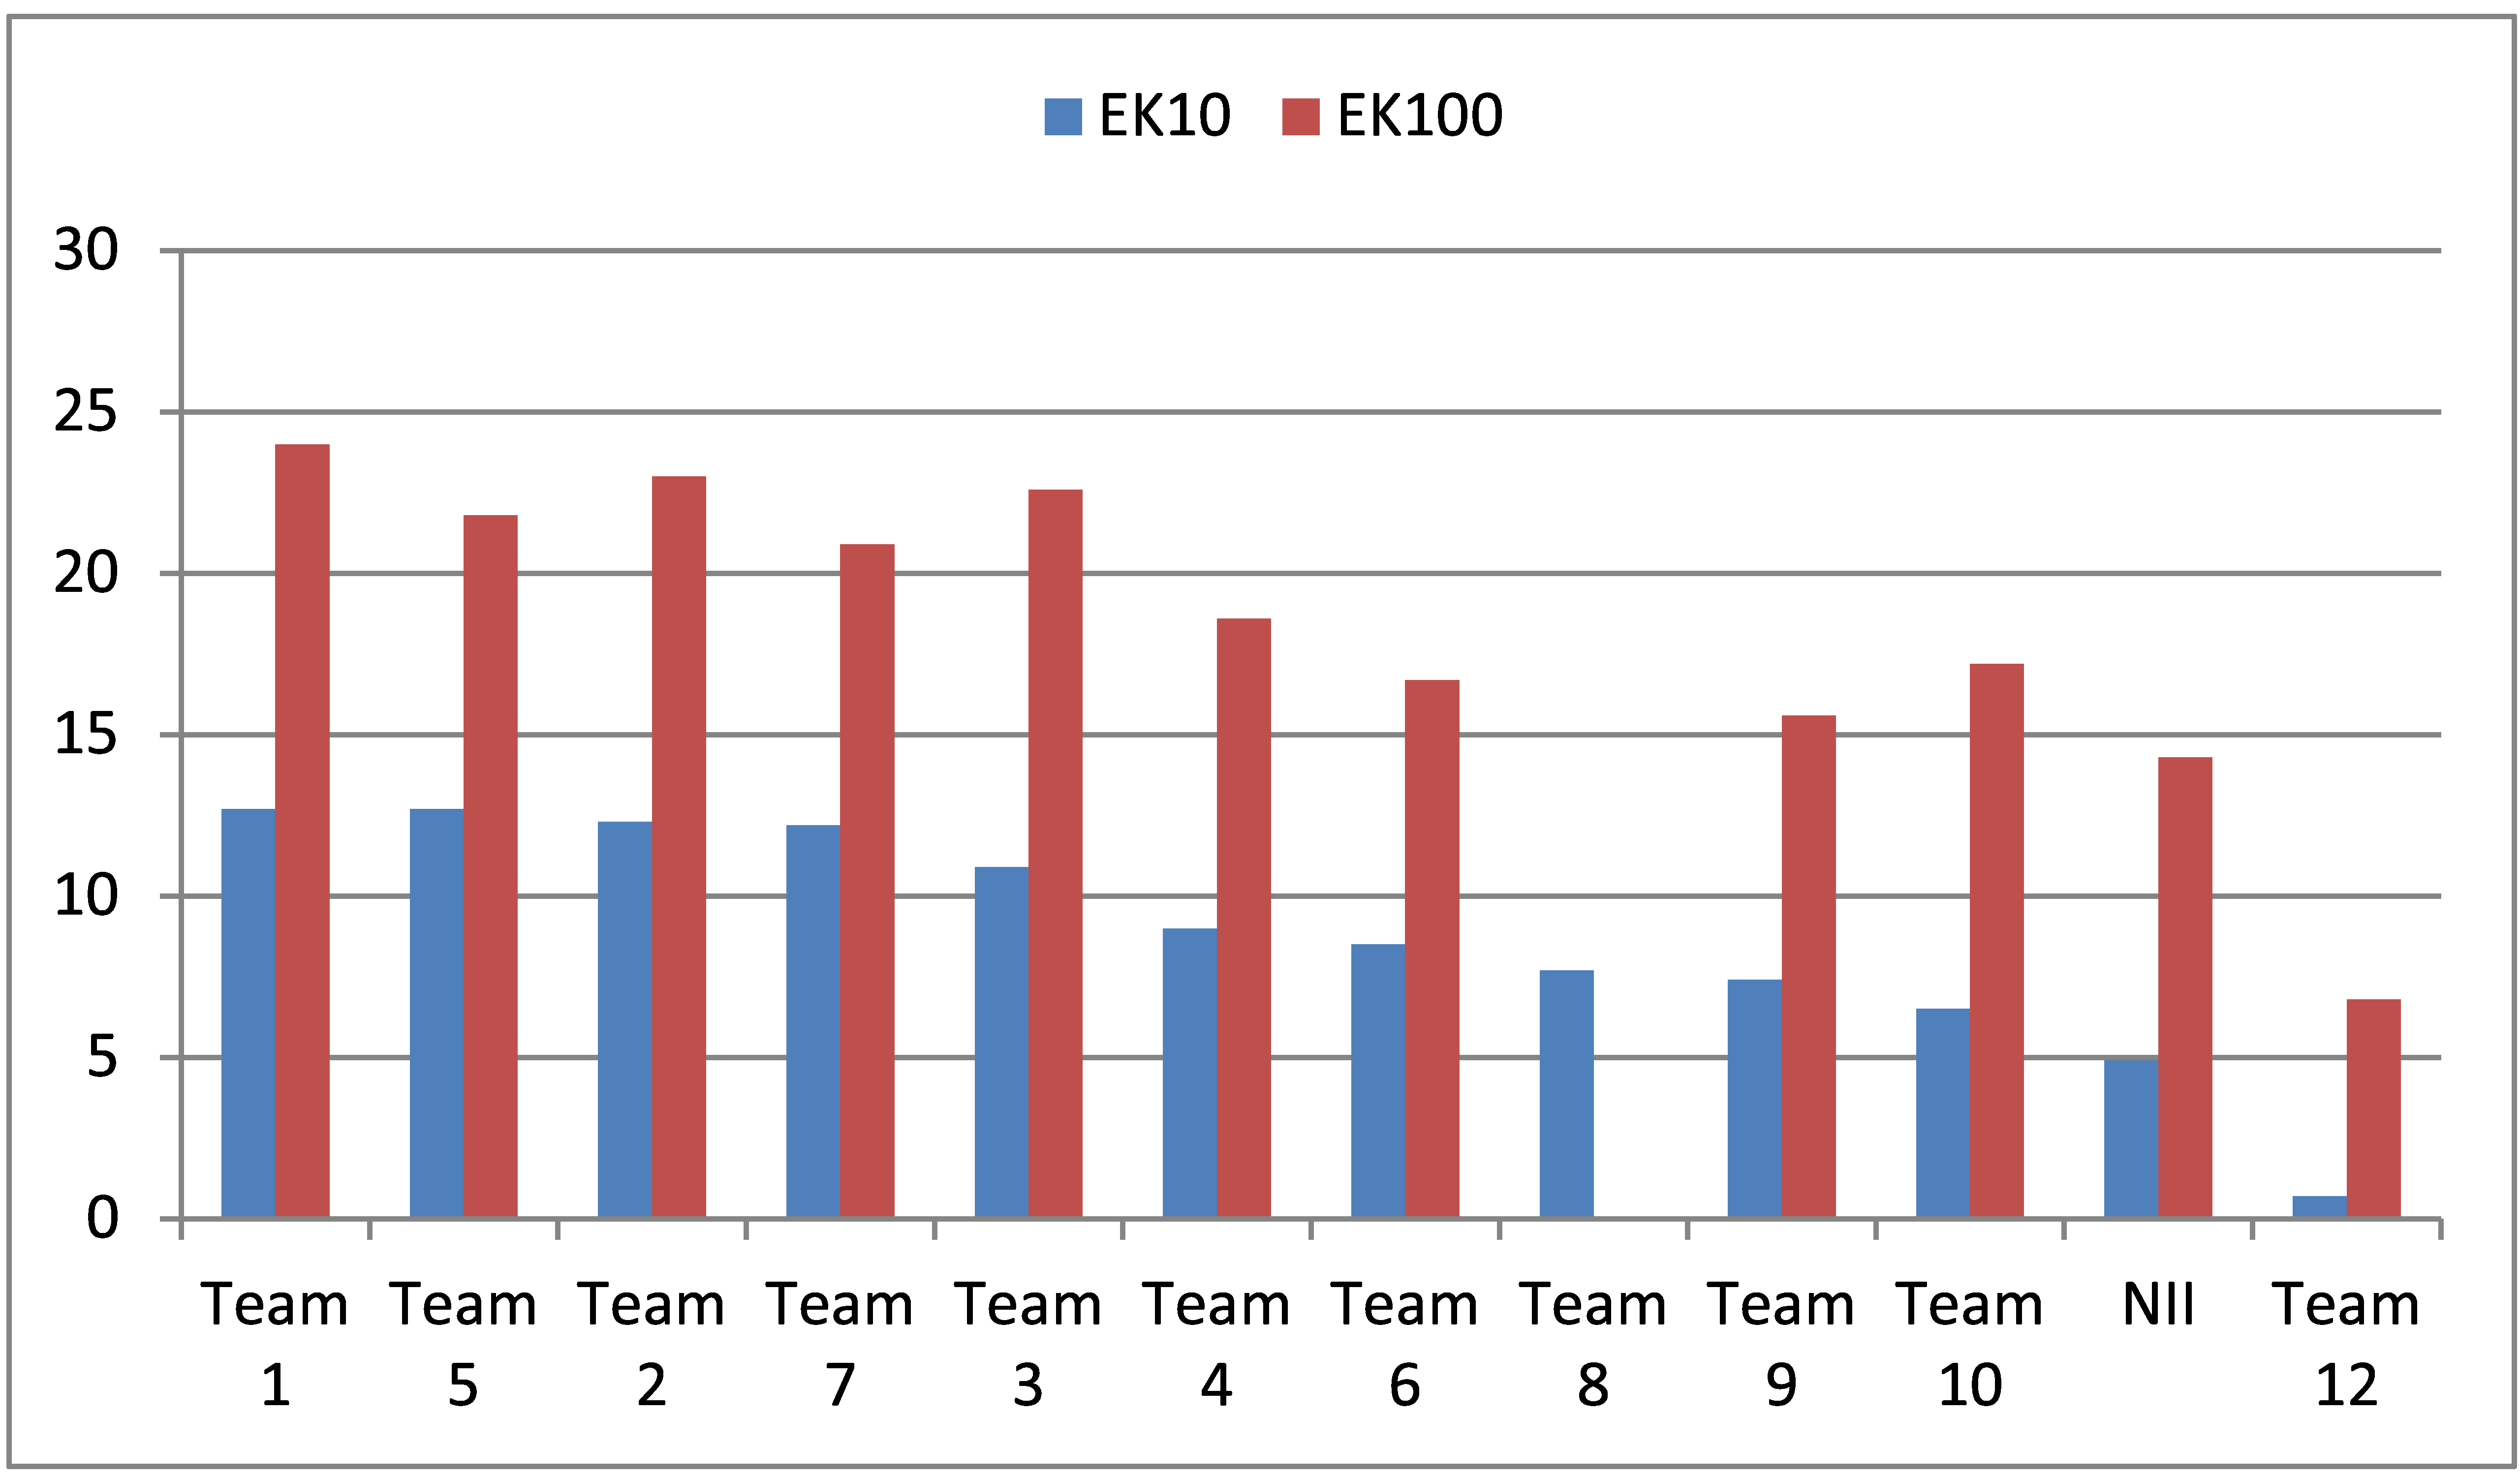
\includegraphics[width=1\linewidth]{med_result_ah.pdf}
		\caption{Ad-Hoc Systems}
		\label{fig_result_ah}
	\end{subfigure}
	\caption{Comparison of our MED system with others on the full evaluation set for both PS and AH tasks. Results are sorted in the descending order of performance on the EK10 setting.}
	\label{fig:results}
\end{figure}




\end{appendices}


\begingroup
\renewcommand\bibname{Publication List}
%\documentclass{article}
\usepackage{natbib}
% whatever you need here, basically a good idea is to use your real thesis header
\begin{document}


	
\cite{phan2014multimedia}

\cite{phan2012codeword}
\cite{PhanNLTLDS12}
\cite{lam2013evaluation}
\cite{lam2013violent}
\cite{ngo2014nii}
\cite{ngo2014recommend}
\cite{phan2014sum}

\cite{lam2012nii}
\cite{lam2013nii}
\cite{lam2014nii}
\cite{le2013nii}
\cite{phannii}
\cite{le2014nii}

\cite{phan2015med}
\cite{nttrang2015}
\bibliographystyle{abbrv}
\bibliography{sangphan}


\end{document}
\clearpage

\begin{thebibliography}{10}

\section*{Journal papers}

\bibitem{phan2014multimedia}
S.~Phan, T.~D. Ngo, V.~Lam, S.~Tran, D.-D. Le, D.~A. Duong, and S.~Satoh.
\newblock Multimedia event detection using segment-based approach for motion
  feature.
\newblock {\em Journal of Signal Processing Systems}, 74(1):19--31, 2014.

\section*{Conference papers}

\bibitem{phan2012codeword}
S.~Phan, V.~Lam, S.~Tran, T.~D. Ngo, D.-D. Le, and S.~Satoh.
\newblock A codeword visualization tool for dense trajectory feature.
\newblock In {\em Multimedia and Expo Workshops (ICMEW), 2012 IEEE
  International Conference on}, pages 672--672. IEEE, 2012.
  
\bibitem{PhanNLTLDS12}
S.~Phan, T.~D. Ngo, V.~Lam, S.~Tran, D.~Le, D.~A. Duong, and S.~Satoh.
\newblock Multimedia event detection using segment-based approach for motion
  feature.
\newblock In {\em Advances in Multimedia Information Processing - {PCM} 2012 -
  13th Pacific-Rim Conference on Multimedia, Singapore, December 4-6, 2012.
  Proceedings}, pages 33--44, 2012.
  
\bibitem{lam2013evaluation}
V.~Lam, D.-D. Le, S.~Phan, S.~Satoh, D.~A. Duong, and T.~D. Ngo.
\newblock Evaluation of low-level features for detecting violent scenes in
  videos.
\newblock In {\em Soft Computing and Pattern Recognition (SoCPaR), 2013
  International Conference of}, pages 213--218. IEEE, 2013.

\bibitem{lam2013violent}
V.~Lam, S.~Phan, T.~D. Ngo, D.-D. Le, D.~A. Duong, and S.~Satoh.
\newblock Violent scene detection using mid-level feature.
\newblock In {\em Proceedings of the Fourth Symposium on Information and
  Communication Technology}, pages 198--205. ACM, 2013.
  
\bibitem{ngo2014nii}
T.~D. Ngo, V.~H. Nguyen, V.~Lam, S.~Phan, D.-D. Le, D.~A. Duong, and S.~Satoh.
\newblock Nii-uit: A tool for known item search by sequential pattern
  filtering.
\newblock In {\em MultiMedia Modeling}, pages 419--422. Springer International
  Publishing, 2014.

\bibitem{ngo2014recommend}
T.~D. Ngo, S.~Phan, D.-D. Le, and S.~Satoh.
\newblock Recommend-me: recommending query regions for image search.
\newblock In {\em Proceedings of the 29th Annual ACM Symposium on Applied
  Computing}, pages 913--918. ACM, 2014.

\bibitem{phan2014sum}
S.~Phan, D.-D. Le, and S.~Satoh.
\newblock Sum-max video pooling for complex event recognition.
\newblock In {\em Image Processing (ICIP), 2014 IEEE International Conference
  on}, pages 1026--1030. IEEE, 2014.


\section*{Technical reports}

\bibitem{lam2012nii}
V.~Lam, D.-D. Le, S.~Phan, S.~Satoh, and D.~A. Duong.
\newblock Nii, japan at mediaeval 2012 violent scenes detection affect task.
\newblock In {\em MediaEval}, 2012.

\bibitem{lam2013nii}
V.~Lam, D.-D. Le, S.~Phan, S.~Satoh, and D.~A. Duong.
\newblock Nii-uit at mediaeval 2013 violent scenes detection affect task.
\newblock In {\em MediaEval}, 2013.

\bibitem{phannii}
S.~Phan, D.-D. Le, and S.~Satoh.
\newblock Nii, japan at the first thumos workshop 2013.

\bibitem{le2013nii}
D.-D. Le, C.-Z. Zhu, S.~Phan, D.~M. Nguyen, V.~Q. Lam, D.~A. Duong, H.~Jegou,
  and S.~Satoh.
\newblock National institute of informatics, japan at trecvid 2013.
\newblock In {\em TRECVID 2013 Workshop}, 2013.

\bibitem{lam2014nii}
V.~Lam, D.~Le, S.~Phan, S.~Satoh, and D.~A. Duong.
\newblock {NII-UIT} at mediaeval 2014 violent scenes detection affect task.
\newblock In {\em Working Notes Proceedings of the MediaEval 2014 Workshop,
  Barcelona, Catalunya, Spain, October 16-17, 2014.}, 2014.

\bibitem{le2014nii}
D.-D. Le, S.~Phan, V.-T. Nguyen, C.-Z. Zhu, D.~M. Nguyen, T.~D. Ngo,
  S.~Kasamwattanarote, P.~Sebastien, M.-T. Tran, D.~A. Duong, and S.~Satoh.
\newblock National institute of informatics, japan at trecvid 2014.
\newblock In {\em TRECVID 2014 Workshop}, 2014.

\end{thebibliography}


\endgroup


% *************************************** Index ********************************

\printthesisindex % If index is present


\end{spacing}

\end{document}
